\documentclass{ifscTCC} % Definicao do documentclass ifscTCC	

% ----------------------------------------------------------
% Informações de dados para CAPA e FOLHA DE ROSTO
% ----------------------------------------------------------
% Identificadores do trabalho - Usados para preencher os elementos pré-textuais
\instituicao[o]{Instituto Federal de Educação, Ciência e Tecnologia de Santa Catarina} % Opcional
\departamento[o]{Departamento Acadêmico de Eletrônica}
\curso[o]{Curso Superior de Engenharia Eletrônica}
\documento[o]{TCC} % [o] para dissertação [a] para tese
\preambulo{Trabalho de conclusão de curso submetido ao Instituto Federal de Educação, Ciência e Tecnologia de Santa Catarina como parte dos requisitos para obtenção do título de engenheiro eletrônico}
\titulo{Pontas de prova de campo próximo em placas de circuito impresso: estudo, desenvolvimento e investigação experimental}

% 1 -> Estudo e caracterização de pontas de prova para obtenção de medidas de campo magnético próximo em análises de compatibilidade eletromagnetica

% 2 -> Pontas de prova de campo próximo em placas de circuito impresso: estudo, desenvolvimento e investigação experimental.


%\subtitulo{Subtítulo (se houver)} % Opcional
\autor{Daniel Henrique Camargo de Souza}
\grau{Bacharel}
\local{Florianópolis} % Opcional (Florianópolis é o padrão)
\data{2019}
%\orientador[Orientador:\\]{Prof. Dr. Luis Carlos Martinhago Schlichting}
%\coorientador[Coorientador\\Universidade ...]{Prof. Dr.}
%\coordenador[Coordenador\\Universidade ...]{Prof. Dr. }

%---------------------------------------------------------------------
% Início do documento
%---------------------------------------------------------------------
\begin{document}
% Retira espaço extra obsoleto entre as frases.
\frenchspacing 

% ----------------------------------------------------------
% CAPA SEGUINDO NORMA TCC IFSC
% ----------------------------------------------------------
%\imprimircapa  %Comando Padrão do Abntex2 (Formato Diferente do IFSC)
\begin{capa}%
    \begin{SingleSpacing}
        \center\ABNTEXchapterfont\bfseries\ INSTITUTO FEDERAL DE EDUCAÇÃO, CIÊNCIA E TECNOLOGIA DE\\SANTA CATARINA - CÂMPUS FLORIANÓPOLIS\\DEPARTAMENTO ACADÊMICO DE ELETRÔNICA\\CURSO SUPERIOR DE ENGENHARIA ELETRÔNICA
        
        \vspace*{3.0cm}     % três espaços simples - conforme norma para TCC do IFSC
        
        \ABNTEXchapterfont\bfseries\MakeUppercase\imprimirautor

        \begin{vplace}[0.5]
            \begin{center}
                \ABNTEXchapterfont\SingleSpacing\bfseries\Large\MakeUppercase\imprimirtitulo
            \end{center}
        \end{vplace}
        
        \begin{center}
            \ABNTEXchapterfont\bfseries\ FLORIANÓPOLIS, 2019
        \end{center}
    \end{SingleSpacing}
\end{capa}

% ----------------------------------------------------------
% FOLHA DE ROSTO SEGUINDO NORMA TCC IFSC
% ----------------------------------------------------------
% Comando Padrão do Abntex2 % (o * indica que haverá a ficha bibliográfica) (Formato Diferente do IFSC)
% \imprimirfolhaderosto*
% \imprimirfolhaderosto
\begin{capa}%
    \begin{SingleSpacing}
        \center
        \ABNTEXchapterfont\bfseries\ INSTITUTO FEDERAL DE EDUCAÇÃO, CIÊNCIA E TECNOLOGIA DE\\SANTA CATARINA - CÂMPUS FLORIANÓPOLIS\\DEPARTAMENTO ACADÊMICO DE ELETRÔNICA\\CURSO SUPERIOR DE ENGENHARIA ELETRÔNICA
        
        \vspace*{3.0cm}     % três espaços simples - conforme norma para TCC do IFSC
        
        \ABNTEXchapterfont\bfseries\MakeUppercase\imprimirautor
        
        %\begin{vplace}[0.5]
        \vspace*{\fill} 
            \begin{center}
                \ABNTEXchapterfont\SingleSpacing\bfseries\Large\MakeUppercase\imprimirtitulo
            \end{center}
        \vspace*{\fill} 
        %\end{vplace}
        
        \hspace{.45\textwidth}
        \begin{minipage}{.5\textwidth}
            \begin{SingleSpacing}
                \normalfont\imprimirpreambulo
                \vspace*{1.0cm}
                
                Orientador:\\Prof. Dr. Luis Carlos Martinhago Schlichting
            \end{SingleSpacing}
        \end{minipage}%
        \vspace*{\fill} 
        
        \begin{center}
            \ABNTEXchapterfont\bfseries\ FLORIANÓPOLIS, 2019
        \end{center}
    \end{SingleSpacing}
\end{capa}

% ----------------------------------------------------------
% FICHA DE IDENTIFICAÇÃO (CATALOGRÁFICA) APROVAÇÃO SEGUINDO NORMA TCC IFSC
% ----------------------------------------------------------
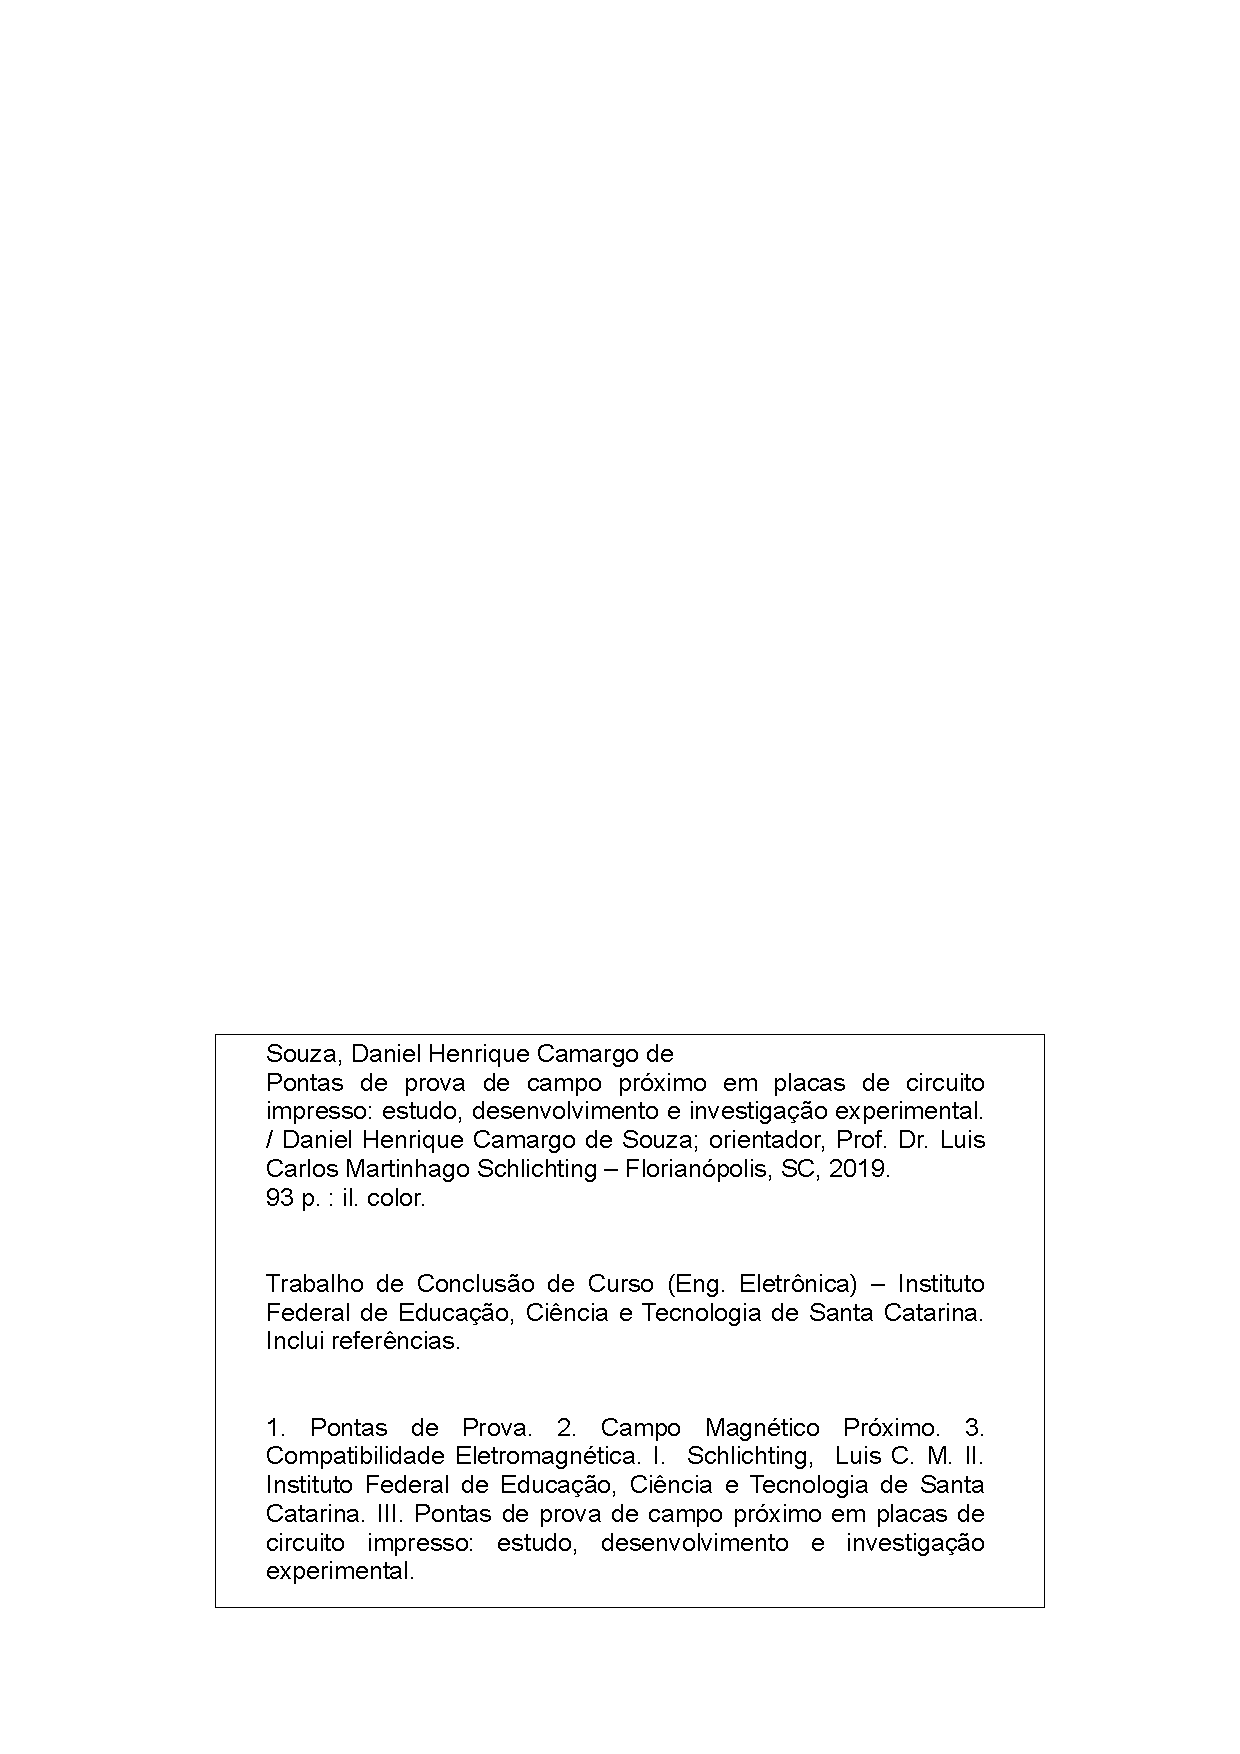
\includepdf{./pdf/fichacatalografica_final.pdf}     %Para Inclusão de modelo fornecido pela Biblioteca
\cleardoublepage

% \begin{fichacatalografica}
%    \sffamily
%    \vspace*{15cm}    % Posição vertical
%    \hrule    % Linha horizontal
%    
%    \begin{center}
%        % Minipage Centralizado
%        \begin{minipage}[c]{12.5cm} % Largura
%            \imprimirautor
%            \hspace{0.5cm} \imprimirtitulo / \imprimirautor. --
%            \imprimirlocal, \imprimirdata-
%            \hspace{0.5cm} \pageref{LastPage} p. : il.(alguma color.); 30 cm.%\\
%            \hspace{0.5cm} \imprimirorientadorRotulo \imprimirorientador\\
%            \hspace{0.5cm}
%            \parbox[t]{\textwidth}{\imprimirtipotrabalho~--~\imprimirinstituicao,
%            \imprimirdata.}\\
%            \hspace{0.5cm}
%            1. Palavra-chave1.
%            2. Palavra-chave2.
%            I. Orientador.
%            II. Universidade xxx.
%            III. Faculdade de xxx.
%            IV. Título\\
%            \hspace{8.75cm} CDU 02:141:005.7\\
%        \end{minipage}
%    \end{center}
%    \hrule
% 
% \end{fichacatalografica}
% ----------------------------------------------------------
% ERRATA SEGUINDO NORMA TCC IFSC (OPCIONAL)
% ----------------------------------------------------------
%\begin{errata}
%    FERRIGNO, C. R. A. \textbf{Tratamento de neoplasias ósseas apendiculares com reimplantação de enxerto ósseo autólogo autoclavado associado ao plasma rico em plaquetas}: estudo crítico na cirurgia de preservação de membro em cães. 2011. 128 f. Tese (Livre-Docência) - Faculdade de Medicina
%    Veterinária e Zootecnia, Universidade de São Paulo, São Paulo, 2011.
%    \begin{table}[htb]
%        \center
%        \footnotesize
%        \begin{tabular}{|p{1.4cm}|p{1cm}|p{3cm}|p{3cm}|}
%            \hline
%            \textbf{Folha} & \textbf{Linha} & \textbf{Onde se lê} &
%            \textbf{Leia-se}\\
%            \hline
%            1 & 10 & auto-conclavo & autoconclavo\\
%            \hline
%        \end{tabular}
%    \end{table}
%\end{errata}
%
% ----------------------------------------------------------
% FOLHA APROVAÇÃO SEGUINDO NORMA TCC IFSC
% ----------------------------------------------------------
\setcounter{page}{4}
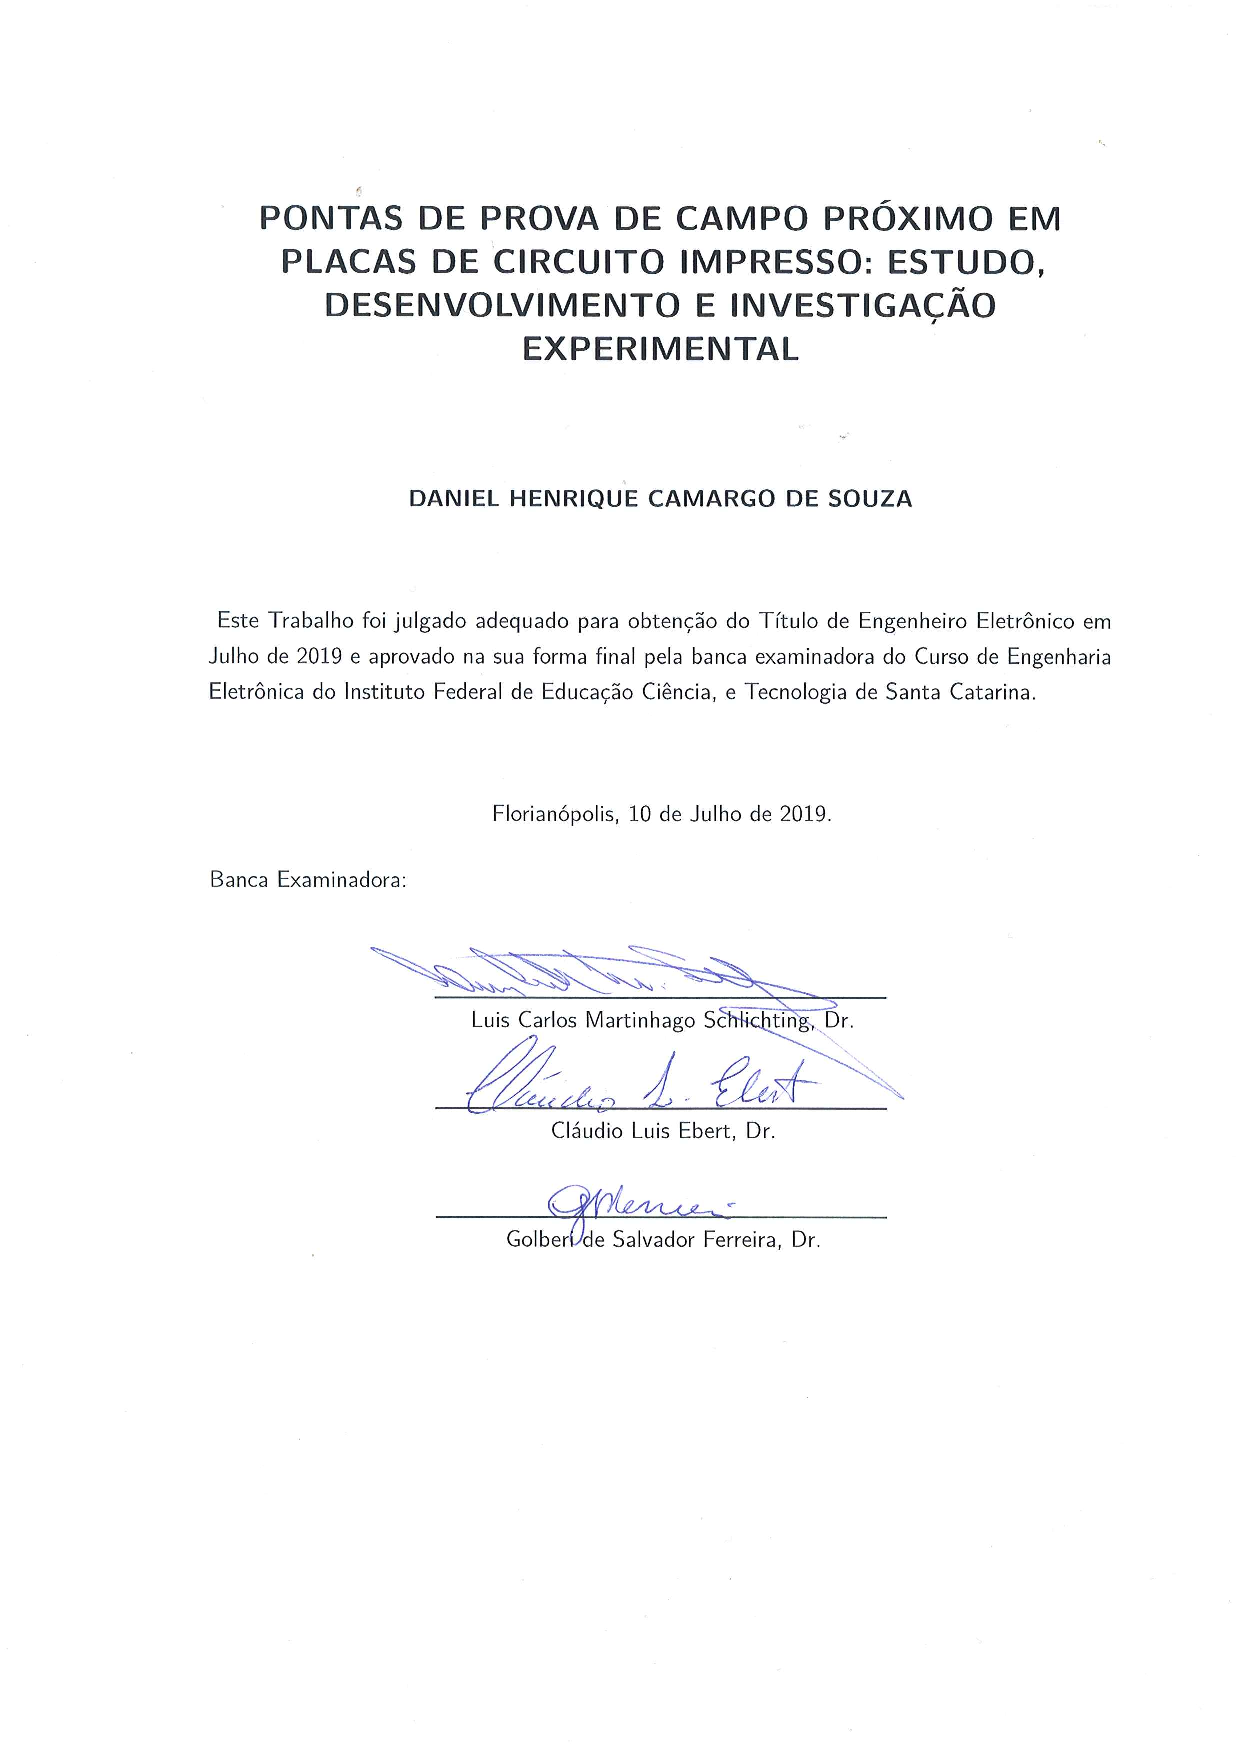
\includepdf{./pdf/folhadeaprovacao_final.pdf}     %Após as assinaturas é incluido digitalizado
% \begin{folhadeaprovacao}
%     \begin{center}
%         \begin{center}
%             \ABNTEXchapterfont\SingleSpacing\bfseries\Large\MakeUppercase\imprimirtitulo
%         \end{center}
%             
%         \vspace*{2.0cm}
%             
%         \ABNTEXchapterfont\normalsize\bfseries\MakeUppercase\imprimirautor
%             
%         \vspace*{1.0cm}
%     \end{center}
%     
%     
%     \noindent\OnehalfSpacing Este Trabalho foi julgado adequado para obtenção do Título de Engenheiro Eletrônico em Julho de 2019 e aprovado na sua forma final pela banca examinadora do Curso de Engenharia Eletrônica do Instituto Federal de Educação Ciência, e Tecnologia de Santa Catarina.
%         
%     \vspace*{1.0cm}
%     \begin{center}    
%         \imprimirlocal, 10 de Julho de 2019.
%     \end{center}
%     
%     \noindent Banca Examinadora:
%     
%     \assinatura{Luis Carlos Martinhago Schlichting, Dr.}
%     \assinatura{Cláudio Luis Ebert, Dr.}
%     \assinatura{Golberi de Salvador Ferreira, Dr.}
% 
% \end{folhadeaprovacao}
\cleardoublepage

% ----------------------------------------------------------
% DEDICATORIA SEGUINDO NORMA TCC IFSC
% ----------------------------------------------------------
% \begin{dedicatoria}
% 
%  \vspace*{20cm}  
%  \hspace*{7cm}
%  Para Voçê
%  
% \end{dedicatoria}


% ----------------------------------------------------------
% AGRADECIMENTOS SEGUINDO NORMA TCC IFSC
% ----------------------------------------------------------
\begin{agradecimentos}
    \begin{itemize}
        \item Aos Colegas de graduação que tornaram a jornada mais um pouco mais agradável e divertida.
        \item Aos Professores do Departamento de Eletrônica do IFSC, pela paciência e dedicação que empenham em seus ensinamentos.
        \item Ao Professor Orientador - Dr. Luis Carlos Martinhago Schlichting (famoso Espirro), pelo suporte, parceria e dedicação em suas orientações e sugestões.
        \item Aos Colegas do LabCEM (IFSC), Pedro Bastos e Arihé Redivo Ramos, por suas sugestões parceria e apoio.
        \item Ao Técnico Fábio Pacheco, pelo suporte, ajuda e presteza sempre que solicitado.
        \item Ao \LaTeX que coloca o Word no chinelo.
    \end{itemize}

\end{agradecimentos}


% ----------------------------------------------------------
% EPIGRAFE SEGUINDO NORMA TCC IFSC
% ----------------------------------------------------------
%\begin{epigrafe}
%	
%    \noindent\textit{‘‘Não vos amoldeis às estruturas deste mundo, \\
%    mas transformai-vos pela renovação da mente, \\
%    a fim de distinguir qual éa vontade de Deus: \\
%    o que é bom, o que Lhe éagradável, o que éperfeito.\\
%    (Bíblia Sagrada, Romanos 12, 2)}
%    
%\end{epigrafe}

% ----------------------------------------------------------
% RESUMO SEGUINDO NORMA TCC IFSC
% ----------------------------------------------------------
% resumo na língua vernácula (obrigatório)
\setlength{\absparsep}{18pt} % ajusta o espaçamento dos parágrafos do resumo

\begin{resumo}
% Passos para um bom RESUMO
% 
% 1 - Explicar tema e relevância
% 2 - Justificativa
% 3 - Objetivo
% 4 - Metodologia (Qualitativo, Quantitativo, Estudo de Caso)
% 5 - Resultados Significativos
% 6 - Breve Conclusão
% 7 - Palavras chaves (no mínimo três)
A Eletrônica é uma área do conhecimento de grande destaque na sociedade moderna. Nos últimos tempos, vem ocorrendo o desenvolvimento de um grande número de sistemas e dispositivos eletrônicos e estes devem estar adequados a padrões de compatibilidade e susceptibilidade eletromagnética. Para verificar se os sistemas e dispositivos eletrônicos estão adequados às normas e padrões exigidos, existem alguns métodos e procedimentos, sendo o foco deste trabalho a técnica de rastreamento de sinal utilizando pontas de provas de campo próximo. Este trabalho objetiva apontar uma via alternativa e de baixo custo para o desenvolvimento de pontas de prova de campo próximo que obtenham medidas satisfatórias visando análises de compatibilidade eletromagnética. Busca-se assim estudar, desenvolver e investigar experimentalmente o funcionamento e características de pontas de prova de campo magnético próximo construídas em placa de circuito impresso. Foram desenvolvidas, ao todo, 20 pontas de provas, e, ao final, conseguiu-se apontar uma alternativa viável com resultados próximos a soluções comerciais existentes.

\noindent
\textbf{Palavras-chaves}: Pontas de Prova, Campo Magnético Próximo, Compatibilidade Eletromagnética. 

\end{resumo}

% ----------------------------------------------------------
% ABSTRACT SEGUINDO NORMA TCC IFSC
% ----------------------------------------------------------
\begin{resumo}[ABSTRACT]
\begin{otherlanguage*}{english}
Electronics is an area of ​​knowledge of great prominence in modern society. The development of a large number of electronic systems and devices has been occuring recently and they must be adapted to standards of compatibility and electromagnetic susceptibility. In order to verify if electronic systems and devices are adequate to the norms and standards required, there are some methods and procedures. The focus of this work is the technique of signal tracing using near field probes. This work aims to point out an alternative and low cost pathway for the development of near field probes that obtain satisfactory measurements for electromagnetic compatibility analysis. The goal is to study, develop and experimentally investigate the operation and characteristics of near field probes built in printed circuit board. A total of 20 near field probes were developed, and, in the end, a feasible solution was found with results close to existing commercial solutions.


\noindent
\textbf{Key-Words}: Near Field Probe, Nearby Magnetic Field, Electromagnetic Compatibility. 
\end{otherlanguage*}
\end{resumo}

% ----------------------------------------------------------
% LISTA DE ILUSTRAÇÕES
% ----------------------------------------------------------
\pdfbookmark[0]{\listfigurename}{lof}
\listoffigures*
\cleardoublepage

% ----------------------------------------------------------
% LISTA DE TABELAS
% ----------------------------------------------------------
\pdfbookmark[0]{\listtablename}{lot}
\listoftables*
\cleardoublepage

% ----------------------------------------------------------
% LISTA DE ABREVIATURAS E SIGLAS
% ----------------------------------------------------------
\begin{siglas}
   \item[EMC] \textit{Electromagnetic Compatibility} - Compatibilidade Eletromagnética
   \item[EMI] \textit{Electromagnetic Interference} -Interferência Eletromagnética
   \item[PCI] Placa de Circuito Impresso
   \item[ESD] \textit{Electrostatic Discharge} - Descarga Eletrostática
   \item[EMP] \textit{Electromagnetic Pulse} - Pulso Eletromagnético
   \item[FCC] \textit{Federal Communication Commission}
   \item[CISPR] \textit{Comité International Special des Perturbations Radioélectriques}
   \item[IEC] \textit{International Electrotechnical Commission}
   \item[LISN] \textit{Line Impedance Stabilization Network}
   \item[NFP] \textit{Near-Field Probe} - Sonda de Campo Próximo
   \item[DUT] \textit{Device Under Test} - Dispositivo Sob Teste
   \item[OATS] \textit{Open-Area Test Site} - Local de Teste de Área Aberta
   \item[SAC] \textit{Semi Anechoic Chamber} - Câmara Semi Anecoíca
   \item[CI] Circuito Integrado
   \item[CC] Corrente Contínua
   \item[CA] Corrente Alternada
   \item[CMOS] \textit{Complementary Metal Oxide Semiconductor} - Semicondutor de metal-óxido complementar
   \item[FR4] \textit{Flame Retardant 4} - Designação de classe para material laminado de epóxi reforçado com vidro utilizado em PCI
   \item[SMD] \textit{Surface-Mount Device} - Componente Montado na Superfície
   \item[SMA] \textit{SubMiniature version A} - Conector Coaxial de RF de $50\Omega$
   \item[IFSC] Instituto Federal de Educação Ciência e Tecnologia de Santa Catarina
%   \item[VDC] \textit{Voltage Direct Current} - Tensão Contínua
%   \item[VAC] \textit{Voltage Alternating Current} - Tensão Alternada
%   \item[ABNT] Associação Brasileira de Normas Técnicas
   \item[abnTex] Normas da ABNT para \LaTeX
   \end{siglas}

% ----------------------------------------------------------
% LISTA DE SIMBOLOS
% ----------------------------------------------------------
\begin{simbolos}
   \item[$V$] Volts - Unidade de potencial elétrico
   \item[$A$] Ampere - Unidade de corrente elétrica
   \item[$\Omega$] Ohms - Unidade de resistência elétrica
   \item[$F$] Faradays - Unidade de capacitância elétrica
   \item[$H$] Henry - Unidade de indutância elétrica
   \item[$W$] Watt's - Unidade de potência elétrica
   \item[$Hz$] Hertz - Unidade de frequência (ciclos por segundo)
   \item[$VA$] Volt-Ampere - Unidade de potência elétrica
   \item[$dB\mu V$] Decibel microVolt - Decibéis relativos a um microVolt
   \item[$dB\mu V/m$] Decibel microVolt por metro - Decibéis relativos a um microVolt por metro
   \item[$mm$] Milimetros - Unidade de comprimento (1 metro divido por Mil)
   \item[$mm^{2}$] Milimetros Quadrados - Unidade de área
   \item[$\,^{\circ}\mathrm{C}$] Grau Celcius - Unidade de temperatura
\end{simbolos}

% ----------------------------------------------------------
% SUMÁRIO
% ----------------------------------------------------------
\pdfbookmark[0]{\contentsname}{toc}
\tableofcontents*
\cleardoublepage

% ----------------------------------------------------------
% ELEMENTOS TEXTUAIS
% ----------------------------------------------------------
\textual

% Cores para os códigos do MatLab
\definecolor{mygreen}{RGB}{28,172,0}    % color values Red, Green, Blue
\definecolor{mylilas}{RGB}{170,55,241}  % o lilas para códigos do MatLab

\lstset{language=Matlab,            %Que tipo de linguaguem os códigos serão
    %basicstyle=\color{red}, 		%normal fontsize
    %basicstyle=\ttfamily\footnotesize 	%fontsize small
    basicstyle=\ttfamily\scriptsize,		%fontsize verysmall
    %breaklines=false,%
    morekeywords={matlab2tikz},
    keywordstyle=\color{blue},%
    morekeywords=[2]{1}, keywordstyle=[2]{\color{black}},
    identifierstyle=\color{black},%
    stringstyle=\color{mylilas},
    commentstyle=\color{mygreen},%
    showstringspaces=false,%without this there will be a symbol in the places where there is a space
    numbers=left,%
    numberstyle={\tiny \color{black}},% size of the numbers
    numbersep=5pt, % this defines how far the numbers are from the text
    emph=[1]{for,end,break},emphstyle=[1]\color{red}, %some words to emphasise
    %emph=[2]{word1,word2}, emphstyle=[2]{style},    
}

% Elimina o Cabeçalho
\pagestyle{parpage}

%\part{Introdução}
\chapter{Introdução}
% Um Pouco da Historia e Evolução da Eletrônica
Certamente a eletrônica é uma área do conhecimento que ganhou muito destaque no último século, com o uso da eletrônica a humanidade produziu adventos tecnológicos que literalmente provocaram mudanças sociais, e, nos dias atuais, produtos (equipamentos e dispositivos) e sistemas eletrônicos ocupam cada vez mais espaço de destaque na vida dos humanos, haja vista a utilização em massa de celulares, computadores, \textit{Smart TVs}, e vários outros produtos eletrônicos. A utilização em massa da eletrônica acarreta no fomento de mais novidades e adventos tecnológicos, criando assim um circulo virtuoso de inovações e consumo, porém este circulo virtuoso pode provocar alguns problemas, como veremos a seguir, principalmente no que se refere a interferências e compatibilidades entre dispositivos eletrônicos.

%Vale ressaltar que mesmo ocorrido uma enorme evolução e uma alta taxa de utilização de eletrônicos ainda ocorre uma alta demanda por produtos e sistemas eletrônicos pelo mundo, isso acarreta no fomento de novidades, fabricantes e sistemas eletrônicos.

% Alta utilização do espectro de frequência (Sistemas)
Com o crescimento da quantidade de novos produtos, fabricantes e sistemas eletrônicos e com uma maior utilização da eletrônica digital no processamento de sinais e dados, os circuitos e sistemas eletrônicos tendem a ter mais pulsos e chaveamentos em suas operações, isso acarreta no aumento de emissões eletromagneticas irradiadas e conduzidas que cada vez mais ocupam um papel de destaque e preocupação dos desenvolvedores de produtos e sistemas eletrônicos.

%evidencia-se um amento no uso de diferentes frequências (diferentes sinais de pulsos e dados, com frequências diferentes de operação), tanto na forma irradiada (rádios, sistemas de comunicação, radares, etc.) quanto na forma conduzida (pulsos, dados, chaveamentos). Esse acréscimo do uso de frequências, gera uma ocupação cada vez maior de um amplo espectro das radiações eletromagnéticas ocasionando um elevado nível de uso dessas radiações nos meios irradiados e conduzidos.

% Susceptibilidade e Interferência dos equipamentos e sistemas eletrônicos
%Em contrapartida, 
Os circuitos eletrônicos precisam atender normas e padrões de qualidade quanto as emissões eletromagneticas irradiadas e conduzidas, e, além disso, devem ser imunes a possíveis interferências das varias emissões que estão a todo momento sendo irradiadas no meio, surge assim uma preocupação latente, para que os produtos e sistemas eletrônicos emitam com intensidades que estejam dentro de limites estabelecidos em normas e que não sejam \textbf{susceptíveis} a interferência de irradiações espúrias que possam estar presente no meio.

% Estudo e análise de compatibilidade eletromagnetica
A área de conhecimento que tem como principal preocupação a busca pelo atendimento das exigências das normas e de Interferência Eletromagnética (\textit{Electromagnetic Interference} - EMI) dos circuitos eletrônicos é a Compatibilidade Eletromagnética (\textit{Eletromagnetic Compatibility} - EMC), onde é estudado métodos e soluções aplicáveis á circuitos eletrônicos no intuito de deixar suas emissões condicionadas aos padrões de normas e regulações e também deixar os circuitos menos susceptíveis a emissões espúrias.

%para isso a EMC busca entender e solucionar os problemas de susceptibilidade e interferência acarretados ou ocasionados pelos circuitos eletrônicos, para isso existe uma gama de técnicas e ferramentas, sendo uma destas a investigação direta, no circuito desejado, através de pontas de provas, da frequência problemática. Esta técnica vem sendo apontada como uma alternativa viável à analises de EMC em circuitos eletrônicos com alta densidade de componentes por $mm^2$. % Densidade eletrônica 
Um dos problemas de EMC, de maior destaque na atualidade é o rastreamento de pontos de emissão de irradiações eletromagnéticas em circuitos eletrônicos com alta densidade de componentes, que ficam agrupados em placas de circuito impresso (PCI) muito proximos, elevando assim a taxa de ocupação por $mm^2$. Esta alta densidade de componentes vem se tornando uma tendência, tanto pelo fato de que os circuitos estão cada vez mais sofisticados e buscam solucionar maiores problemas, quanto pelo fato da miniaturização desses circuitos, portanto, quanto maior a densidade de componentes maior é o desafio tecnológico proposto.


%isso acarreta em um desafio ao estudo da EMC, pois há a necessidade de criação de métodos que trabalhem com dimensões cada vez menores.
% Identificar a fonte de EMI 

% Ponta de Provas para Campo-Proximo

% Comentar o que será tratado em cada capitulo
Estudos como o de \cite{sivaraman2017} apontam na direção do desenvolvimento de pontas de provas, para a obtenção de medidas de campo próximo afim de proporcionar uma ferramenta mais adequada para análises de EMC em circuitos com alta densidade de componentes eletrônicos. Diante disso, este trabalho visa trazer uma contribuição para o desenvolvimento no IFSC de pontas de prova de campo próximo (\textit{Near Field Probe} - NFP) em placas de circuito impresso que sejam de fácil construção e de baixo custo a serem aplicadas em análises de EMC.

%Apontar os estudos na área para criação de pontas de provas
%O desenvolvimento de instrumentos para medir campos próximos não é nada recente, em 
%An Overview of Near-Field Antenna Measurements
%\cite{yaghjian1986} já temos uma revisão sobre este assunto. porém com o passar dos anos e com a evolução da eletrônica e sua tendência à miniaturização o assunto se tornou cada vez mais frequênte e relevante. em 
%Standard Probes for Electromagnetic Field Measurements
%\cite{kanda1993} temos um estudo que aponta na direção das pontas de provas como solução para obtenção de medidas de campo próximo. 

%Nota-se em 
%Design of magnetic probes for near field measurements and the development of algorithms for the prediction of EMC
%\cite{sivaraman2017} uma preocupação recente na busca por pontas de provas fáceis de serem contruidas e caracterizadas. É nessa linha que se propõe-se seguir neste trabalho, estudar e caracterizar pontas de provas de baixo custo e fácil construção a serem aplicadas na obtenção de medidas de campo magnético próximo em análises de EMC.

A partir deste trabalho, existe a intenção do desenvolvimento, também no IFSC, de um sistema automatizado de rastreamento de sinais em placas de circuitos eletrônicos, utilizando as NFP desenvolvidas neste trabalho, este sistema automatizado contribuiria significativamente para a eficiência das análises de EMC no IFSC, haja vista que hoje os rastreamentos dos sinais são realizados manualmente, o que demandam muito tempo de horas trabalhadas. 

Este trabalho foi divido em 7 capítulos assim dispostos. No capitulo 2 será discorrido sobre a fundamentação teorica que está por tráz da análise de EMC e do desenvolvimento de NFP, sua caracterização e estudo. No capitúlo 3 aborda-se-á a respeito do estudo das caracteristicas das NFP, seus aspectos de modelagem eletromagnética. No capitúlo 4 será demonstrado a metodologia e os procedimentos utilizados na investigação experimental das NFP desenvolvidas. No capitúlo 5 se disocorrer-se-á sobre as caracteristicas levantadas. E por fim, No capitúlo 6 será trazido a tona possiveis aplicações futuras, considerações finais e as conclusões.

\section{Justificativa}
% uma forma rápida e precisa de investigar os focos de emissão de radiação é através das pontas de provas (comentar do sistema de varreduda eletronico e automatico para este processso) 
\citeonline{sivaraman2017} aponta que uma forma eficaz para investigar problemas de EMI e efetuar análises de EMC em circuitos eletrônicos é através do rastreamento de sinais utilizando NFP, no intuito de identificar o exato ponto nesses circuitos de onde a emissão ocorre. 

%Certamente, um profissional qualificado utilizando alguma ponta de prova, terá a capacidade de identificar, de forma satisfatória e relativamente rápida, o ponto exato da emissão investigada. Porém, com a alta demanda de desenvolvimento, e com a tendência de miniaturização dos circuitos eletrônicos, nem sempre haverá algum profissional para realizar uma análise precisa e satisfatória.

Este trabalho visa apontar uma via alternativa e de baixo custo (utilizando para isso topologias em leiautes de placas de circuito impresso) para o desenvolvimento de NFP que obtenham medidas satisfatórias de campo próximo. Além disso este trabalho poderá servir de base para o desenvolvimento de ferramentas automatizadas para análises de EMC, dispensando assim recurso humano e podendo tornar o processo mais rápido e eficaz.

% Pontas de provas comerciais são caras
% 1) Uma forma rápida de obter pontas de provas
% 2) Ponta de Prova de baixo custo. Comparar com modelos comercias
% 3) Altissima plasticidade nas topologias. Pode-se desenhar, projetar uma gama alta de topologias, Redes ou sistemas de pontas de provas

% além disso prover uma ponta de prova mais barata de de fácil fabricação

\section{Definição do Problema}
O problema principal deste trabalho consiste em responder o seguinte questionamento. É possível apontar uma solução de leiaute para o desenvolvimento de NFP, em placas de ciruito impresso (PCI), que obtenham medidas de campo próximo afim de realizar o rastreamento de sinais em placas de circuitos eletrônicos?

\section{Objetivos}

% 3 Diametros (Face Simples) (Sem e Com Plano Terra)
% 3 Diamentro (Face Dupla)  (Sem e Com Plano Terra)

\subsection{Objetivo Geral}
De forma direta tem-se como objetivo:

\begin{itemize}
\item Estudar, desenvolver e investigar experimentalmente topologias em placas de circuito impresso para pontas de prova de campo próximo que sejam eficientes e de baixo custo para a obtenção de medidas de campo magnético próximo em análises de compatibilidade eletromagnética.
\end{itemize}

% Estudar e caracterizar desenhos eficientes e de baixo custo de pontas de prova para a investigação de EMC em placas de PCI

Para alcançar tal objetivo geral elencou-se alguns objetivos especificos.

\subsection{Objetivos Específicos}

\begin{alineas}
\item Estudar o modelo eletromagnético das pontas de provas.
\item Implementar topologias de pontas de provas em placas de circuito impresso.
\item Caracterizar a resposta em frequência de pontas de provas impressas em PCI.
\item Investigar a resolução espacial das pontas de provas.
\item Investigar a influência do tamanho do raio da espira na sensibilidade das pontas de provas.
\item Investigar a influência do número de espiras na sensibilidade e resolução espacial das pontas de provas.
\item Investigar a influência do plano de terra (ou plano de referência) na resolução espacial, sensibilidade e largura de banda das pontas de prova.
%\item Identificar e mensurar parametros essencias das pontas de provas nas difentes topologias (Fator de Antena, Sensitividade, Seletividade, Resolução Espacial e Largura de Banda).
\item Comparar quantitativamente e qualitativamente as diferentes topologias.
%item Implementar uma rede de pontas de provas para obtenção de medidas de campo magnético proximo.
%\item Caracterizar a resposta em frequência da rede de pontas de provas impressa em PCI
%\item Identificar e mensurar parametros essencias da rede de pontas de provas (Fator de Antena, Sensitividade, Seletividade, Resolução Espacial e Largura de Banda).
%\item Comparar quantitativamente e qualitativamente a rede de pontas de provas com a topologia de ponta de prova única.
\item Comparar qualitativamente a resposta em frequência e largura de banda das pontas de provas desenvolvidas com outras soluções comerciais.
\end{alineas}

\chapter{Fundamentação Teórica} \label{fundamentacao}
Neste capitulo será discutido as teorias que embasam a compatibilidade eletromagnética, quais as problematizações que são inerentes em análises de compatibilidade eletromagnética, as formas como estas são realizadas. Especificamente será abordado o estudo da compatibilidade eletromagnética em PCIs. %, quais medidas são realizadas e que tipos de técnicas se encontram no estado da arte nesta realização.

\section{Compatibilidade Eletromagnética}
% Aspectos Gerais da EMC
Desde o advento das comunicações telegráficas e do rádio até os dias atuais com sistemas muito mais complexos de comunicação (radares, estações de rádio, TV, telefonia móvel, satélites), e, cada vez mais sendo utilizados sistemas eletrônicos (dispositivos, equipamentos, etc...) a interferência eletromagnética é tema de interesse e estudo de cientistas e engenheiros das áreas de comunicações e eletricidade~\cite[p.~1]{paul2006}.

Segundo~\citeonline[p.~3]{paul2006} o estudo da Compatibilidade Eletromagnética (EMC) se concentra em investigar três aspectos fundamentais: \textit{Geração, Transmissão e Recepção} de sinais eletromagnéticos. A interação dos sinais gerados no transmissor com o receptor pode interferir no receptor ou até mesmo em si próprio (transmissor), esta interferência pode gerar uma não compatibilidade eletromagnética (porém isso não necessariamente é sempre válido) quando esta interferência acarreta em mal funcionamento em si próprio (transmissor) ou no receptor (ou em demais equipamentos eletrônicos) é necessário uma correção na exata fonte do sinal indesejado, para isso são necessários métodos de investigações afim de identificar com precisão esta fonte. O tipo de transmissão que leva a esta \textit{interferência} define o tipo de acoplamento, ou por meios de sinais eletromagnéticos conduzidos, ou por meios de sinais eletromagnéticos irradiados.

Na figura~\ref{fig:EMC_couplling_problem} ~\citeonline[p.~3]{paul2006} traz de forma sintética esses três principais aspectos no estudo da compatibilidade eletromagnética, a fonte ou emissor (\textit{source}) produz a emissão que é transmitida através do acoplamento (meio pelo qual a emissão é acoplada, ou de forma conduzida ou irradiada) até o receptor.

\begin{figure}[htb!]
	\centering 
	\caption{Aspecto Geral do Estudo de EMC}
	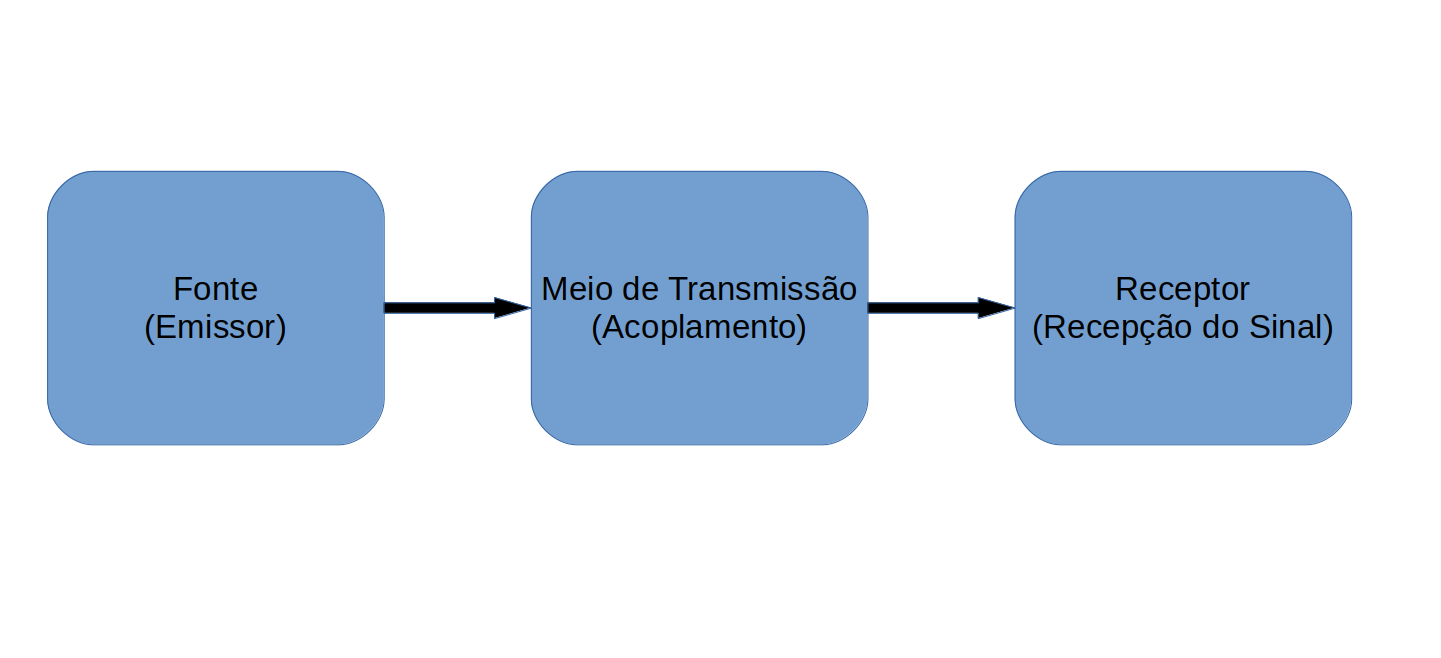
\includegraphics[scale=0.4]{./img/fundamentacao_001}
	\fonte{Adaptado de ~\citeonline[p.~3]{paul2006}}
	%\legend{\hspace{-218pt}Fonte:~\citeonline[p.~3]{paul2006}}
	\label{fig:EMC_couplling_problem}
\end{figure}

Uma das principais preocupações do estudo da EMC está em atender as normas legais e requisitos impostos pelas agências reguladoras, entretanto há também vários outros aspectos importantes a serem explorados pelo estudo de EMC. Na figura~\ref{fig:EMC_preocups} ~\citeonline[p.~8]{paul2006} traz alguns outros problemas importantes a serem investigados pelo estudo de EMC, podemos observar na figura~\ref{fig:EMC_preocups}(a) um problema de susceptibilidade muito comum nos dias atuais que é o da descarga eletrostática (\textit{Electrostatic Discharge} - ESD), onde o indivíduo se carrega eletrostaticamente e libera esta carga através do contato com equipamentos eletrônicos, podendo ocasionar assim mal funcionamento, deformidades ou até a destruição permanente do equipamento eletrônico, principalmente em sistemas ou equipamentos eletrônicos que utilizam Circuito Integrados (CI's). 

\begin{figure}[htb!]
	\centering 
	\caption{Outras Preocupações em EMC}
	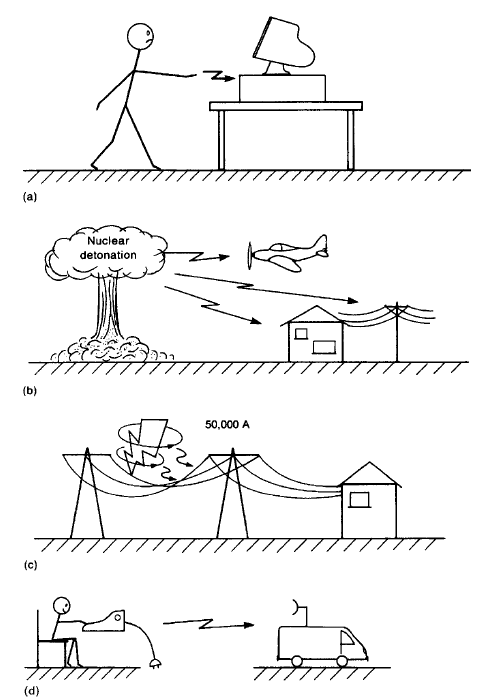
\includegraphics[scale=0.75]{./img/fundamentacao_002}
	\fonte{~\citeonline[p.~8]{paul2006}}
	%\legend{\hspace{-218pt}Fonte:~\citeonline[p.~8]{paul2006}}
	\label{fig:EMC_preocups}
\end{figure}

Ainda na figura~\ref{fig:EMC_preocups} o autor \cite[p.~8]{paul2006} traz demais preocupações do estudo de EMC, como exposto em (b) o efeito de radiações nucleares e dos pulsos eletromagnéticos (EMP) em sistemas eletrônicos embarcados, como de aviação, satélites (radiações espaciais). Em (c) temos os possíveis efeitos causados por tempestades de raios que provocam correntes na ordem $50000 A$ ocasionando campos eletromagnéticos de alta intensidade, podendo assim gerar Interferências Eletromagnéticas (EMI) em equipamentos e sistemas eletrônicos. Por fim em (d) temos a interceptação eletromagnética não autorizada, sendo a área militar e de comunicações possuidoras do maior interesse tanto na prevenção quanto na implementação.

% Historia Rápida da EMC
\subsection{Evolução temporal da EMC}
Muito provavelmente a EMI e sua correção surgiu como algo de interesse com os experimentos de Marconi no final do séc XIX~\cite[p.~10]{paul2006}. Porém, somente a partir do séc XX, na década de 1920, é que começaram a surgir artigos científicos que tratavam da EMI em rádios, tanto nos transmissores quanto nos receptores.

Durante a II Guerra Mundial, o uso de equipamentos eletrônicos, principalmente rádios, dispositivos de navegação, radares e aceleradores, ocasionou um aumento significativo por correções afim de eliminar as EMI principalmente entre rádios e aviões. Entretanto, o crescimento mais significativo das EMI ocorreu a partir do advento do transistor, na década de 1950, do Circuito Integrado (CI), na década de 1960 e do microprocessador, na década de 1970. O espectro de frequência também foi afetado, com uma maior demanda e utilização, após o crescimento da demanda por transmissão de voz e dados, isto começou a exigir maiores esforços no planejamento e regulação da utilização do espectro, o que continua até nos dias atuais ~\cite[p.~10]{paul2006}.

% Requisitos Governamentais
% Falar das Normas
Talvez o principal evento que trouxe a EMC ao nível atual de ênfase, foi a introdução do processamento digital de sinais e computação que no inicio da década de 1960 utilizavam as válvulas à vácuo, porém poucos anos mais tarde, estas foram substituídas por transistores e CI's. Com a inserção da eletrônica de estado sólido no processamento digital de sinais e computação, aumentou-se a velocidade de processamento (chaveamento) e a miniaturização dos componentes ocasionando uma aumento do espectro de frequências utilizável e uma densidade maior de \textit{ruídos} e EMI. Devido ao aumento de novos ruídos e EMI, tanto através do modo conduzido como do irradiado a \textit{Federal Communications Commision} (FCC) publicou em 1979, nos Estados Unidos, uma regulamentação para a emissão eletromagnética em todos os dispositivos digitais até certos limites. A principal intenção dessa regulamentação era trazer limites a "\textit{poluição eletromagnética}". Todavia, na Europa, já haveria ocorrido ações similares, precedentes à FCC. Já em 1933 a \textit{International Electrotechnical Commission} (IEC), em Paris na França, recomendou a criação da \textit{Comité International Special des Perturbations Radioélectriques} (CISPR). ~\citeonline[p.~11]{paul2006} salienta que "A CISPR voltou a se reunir após a Segunda Guerra Mundial em Londres em 1946. Reuniões subsequentes renderam várias publicações científicas, que abordavam com técnicas de medição, bem como limites de emissão recomendados. Alguns países europeus adotaram versões de limites recomendados pela CISPR." Sendo assim, a CISPR e a FCC se tornaram desde então as maiores precursoras de regulamentações e regras no que tange a EMI em nível global.

As regulamentações tanto da FCC quanto da CISPR tornaram a EMC uma aspecto importante para a comercialização de equipamentos e sistemas eletrônicos, visto que se estes não estiveram em conformidade com essas regulações, não poderão ser comercializados nos países que as adotam, mesmo levando-se em conta que o produto realiza sua tarefa e os clientes não se importam se o produto cumpre ou não a regulamentação estabelecida. Dessa forma, as regulamentações estatais tornaram a EMC um aspecto de suma importância no desenvolvimento de produtos e sistemas eletrônicos \cite[p.~12]{paul2006}.

\subsection{Requisitos de EMC em sistemas eletrônicos}
% Requisitos de funcionamentos de sistemas Eletrônicos 2.1(paul2006)
Basicamente há duas classes de requisitos a serem observadas no desenvolvimento de produtos/sistemas eletrônicos afim de atender a EMC, sendo estes ~\cite[p.~49]{paul2006}:

\begin{itemize}
 \item Requisitos Governamentais, Normas e Leis
 \item Requisitos Funcionais, Susceptibilidades e EMI
\end{itemize}

% Requisitos Governamentais (FCC e CISPR) 2.1(paul2006)
Devido ao estágio atual de globalização é de suma importância para os fabricantes e desenvolvedores de produtos eletrônicos estarem atentos as normas e regulamentações, tando da FCC quanto da CISPR. Nos Estados Unidos é adotado as normas da FCC~\cite{fcc47} que estabelece regulações para o rádio e comunicações cabeadas. A FCC estabelece que qualquer equipamento capaz de emitir energia, tanto por radiação quanto conduzida, estando entre $9kHz$ até $3000 GHz$ é um equipamento de rádio-frequência sujeito assim ao capitulo 15 da 47CFR ~\apud[p.~50]{fcc47}{paul2006}, na FCC ainda está definido o que é dispositivo digital:

\begin{citacao}[english]
Any unintentional radiator (device or system) that generates and uses timing pulses at a
rate in excess of 9000 pulses (cycles) per second and uses digital techniques \apud[p.~51]{fcc47}{paul2006}.
\end{citacao}

Ou seja, qualquer equipamento ou sistema de rádio-frequência que gerar ou usar pulsos de tempo que sejam superiores a $9kHz$ e que usa técnicas digitais é considerado pela FCC como um dispositivo digital. Esta definição é importante pois a FCC classifica esses produtos em duas classes: \textbf{Classe A}: São aqueles fabricados para uso comercial, industrial ou destinado a negócios; \textbf{Classe B}: são aqueles fabricados para o uso residencial ~\cite[p.~51]{paul2006}, computadores pessoais e seus periféricos são uma subcategoria de dispositivos digitais de Classe B. Os limites de emissão eletromagnética estabelcidos à Classe B são mais rigorosos do que os limites da Classe A pois supõe-se que a interferência de dispositivos em um ambiente industrial pode ser corrigida mais facilmente do que em um ambiente residencial, onde a fonte de interferência e o dispositivo susceptível estão mais próximos. Esta classificação também é adotada pela CISPR.

% EMC Conduzida e Irradiada
A FCC possui regras que estabelecem limities máximos permitidos às emissões conduzidas e irradiadas do produto digital. Emissões conduzidas são aquelas trasmitidas através de um meio condutor, um cabo, uma trilha de circuito eletrônico, etc. A faixa de freqüência para emissões conduzidas se estende de $150 kHz$ a $30 MHz$. As irradiadas são aqueles cujo o meio de transmissão é o ar ou o vácuo, ou seja, através de radiações eletromagnéticas e a faixa de frequência estabelecida pela FCC para esse tipo de emissão é de $30 MHz$ a $40 GHz$. As mesmas faixas são adotadas também pela CISPR.

A conformidade dos circuitos eletrônicos é verificada, no caso das emissões conduzidas, inserindo-se uma rede estabilizada de impedância de linha (\textit{Line Impedance Stabilization Network} - LISN) no cabo de alimentação em corrente alternada (CA) da unidade. Embora a emissão a ser controlada esteja passando em corrente CA no cabo da linha, os limites são dado em volts ($V$). Isso ocorre porque o dispositivo de teste (LISN) mede uma tensão que está diretamente relacionada à corrente de interferência. No caso das emissões irradiadas, a FCC, assim como outras agências reguladoras, incluindo a CISPR, exige a medição do campo elétrico irradiado, e os limites regulatórios são dados em termos desse campo em decibél de micro Volt por metro quadrado ($dB\mu V/m^2$). as emissões irradiadas devem ser medidas com a antena de medição nas polarizações vertical e horizontal em relação ao plano de terra do local de teste e o produto deve estar em conformidade para as duas polarizações~\cite[p.~52]{paul2006}.

Os limites para as emissões conduzidas dos equipamentos da classe B podem ser visualizados na tabela~\ref{tab:TABLE_Conduzida_ClasseB} enquanto que os limites das emissões conduzidas dos equipamentos da class A podem ser vistos na tabela~\ref{tab:TABLE_Conduzida_ClasseA}.

\begin{table}[htb!]
  \centering
  \caption{FCC e CISPR 22 - Limites para Emissão Conduzida (Classe B)}
  \label{tab:TABLE_Conduzida_ClasseB}
  \begin{tabular}{|c|c|c|}
\hline
%\multicolumn{3}{|c|}{\textbf{Parâmetros}}\\	\hline
Frequência (MHz)    &   $\mu V$ QP (AV) &   $dB\mu V$ QP (AV)\\	\hline\hline
0,15	&	1995(631)	&	66(56)	\\	%\hline
0,5	&	631(199,5)	&	56(46)	\\	%\hline
0,5 – 5	&	631(199,5)	&	56(46)	\\	%\hline
5 – 30	&	1000(316)	&	60(50)	\\	\hline
  \end{tabular}
  \fonte{~\citeonline[p.~52]{paul2006}}
\end{table}

Nas tabelas apresentadas vemos que há dois níveis que devem ser satisfeitos, o nível Quasi-Pico (QP) e o nível da média - \textit{Averange}(AV).

\begin{table}[htb!]
  \centering
  \caption{FCC e CISPR 22 - Limites para Emissão Conduzida (Classe A)}
  \label{tab:TABLE_Conduzida_ClasseA}
  \begin{tabular}{|c|c|c|}
\hline
%\multicolumn{3}{|c|}{\textbf{Parâmetros}}\\	\hline
Frequência (MHz)    &   $\mu V$ QP (AV) &   $dB\mu V$ QP (AV)\\	\hline\hline
0,15 - 0,5	&	8912,5(1995)	&	79(66)	\\	%\hline
0,5 - 30	&	4467(1000)	&	73(60)	\\	\hline
  \end{tabular}
  \fonte{~\citeonline[p.~53]{paul2006}}
\end{table}

Quanto as emissões irradiadas, na figura~\ref{fig:irradiada_limites} podemos visualizar os limites estabelecidos por ambas as normas FCC e CISPR 22 para os equipamentos da Classe A e Classe B, sendo que para a FCC as emissões irradiadas dos equipamentos da Classe B são medidas a uma distância de 3m, e, 10m para os Classe A.

\begin{figure}[htb!]
	\centering
 	\caption{FCC e CISPR 22 - Limites para emissão irradiada}
 	\label{fig:irradiada_limites}
	\subfloat[][Limites emissão irradiada - Classe B]{
		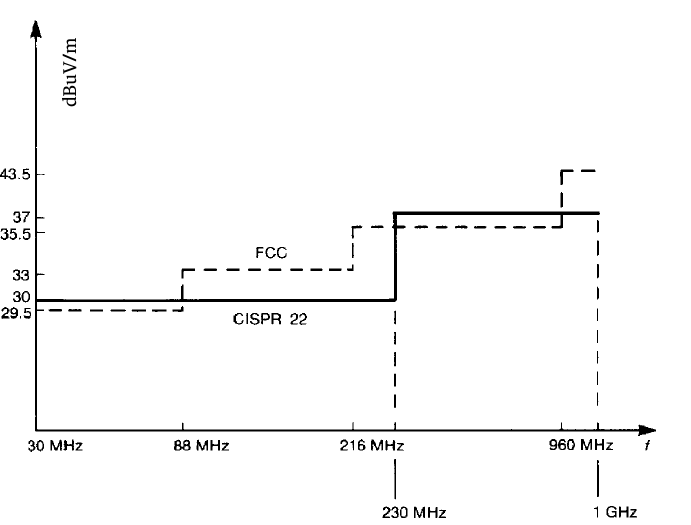
\includegraphics[scale=0.45]{./img/FCC_CISPR_10m_classB}}
	\subfloat[][Limites emissão irradiada - Classe A]{
		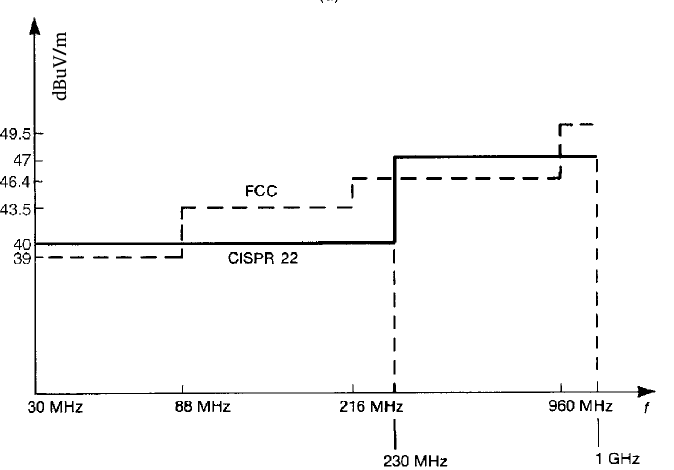
\includegraphics[scale=0.5]{./img/FCC_CISPR_10m_classA}}
    \fonte{Adaptado de~\citeonline[p.~55]{paul2006}}
\end{figure}

A maioria dos requisitos governamentais de EMC para mercados fora dos Estados Unidos Estados são estabelecidos pelo "\textit{Comité International Special des Perturbations Radioélectriques} - (CISPR), que é um comitê da International Electrotechnical Commission (IEC). Embora a CISPR escreva padrões, eles não são obrigatórios. No entanto, a maioria países internacionais adotam as recomendações da CISPR. O mais amplamente utilizado padrão é o CISPR 22, que estabelece limites para as emissões irradiadas e conduzidas de equipamento de tecnologia da informação, que inclui basicamente dispositivos digitais
no significado semelhante ao da FCC. Os limites são divididos em Classe A e Classe B, e seu significado é essencialmente o mesmo que as definições da FCC~\cite[p.~55]{paul2006}.

% Requisitos Funcionais (Susceptibilidades) 2.2(paul2006)
Como mencionado anteriormente, não é inteligente projetar um produto que realize alguma
função comercial sem que este não cumpra os requisitos regulamentares de EMC. Similarmente, também não é inteligente projetar um produto que atenda aos requisitos regulamentares de EMC estabelecidos pelas agências governamentais, mas não funcionar satisfatoriamente quando colocado perto de um transmissor de rádio FM ou de um radar de vigilância aeroportuária. Os consumidores não irão se satisfazer caso haja problemas causados por esses emissores no funcionamento dos dispositivos. Eles esperam que um produto que foi adquirido de boa fé funcione satisfatoriamente em qualquer instalação residencial, e o consumidor também não ficará satisfeito se houver um aviso que afirma “Cuidado, este computador não funcionará se sua casa estiver em um raio de 1 km de uma torre de transmissão FM"~\cite[p.~79]{paul2006}.. 

Igualmente embaraçoso seria se algum produto funcionar adequadamente, porém se o operador, através de um tapete de nylon em um escritório situado em um clima seco, toca o produto, causando uma descarga eletrostática que reinicializa a máquina. Por isso releva-se a importância do fabricante de impor determinados testes para além dos necessários por agências governamentais, a fim de garantir que o produto funcione adequadamente em uma ampla variedade de instalações de campo~\cite[p.~79]{paul2006}. 

\section{Análises de EMC em Placas de Circuito Impresso}
Os equipamentos eletrônicos são fabricados em 99,9\% dos casos utilizando uma placa de circuito impresso (PCI), sendo assim, é de extrema importância conhecer métodos e técnicas de análise de EMC em PCIs, para além disso, também conhecer soluções de leiaute e de fabricação destas placas, afim de minimizar o impacto e custos de correções destinadas a melhorias da compatibilidade eletromagnética.

% Como é feito as analises de EMC em Placas
As emissões eletromagnéticas de uma PCI são classificadas como emissões conduzidas e irradiadas ou emissões em modo comum e modo diferencial. As medidas das emissões conduzidas são realizadas com o uso de uma LISN, como visto anteriormente. Quanto as medições de emissões irradiadas, existem vários métodos de análises disponíveis~\apud[p.~12]{sivaraman2017}{hoolihan2017}, sendo que o método de maior interesse neste trabalho é o método de varredura de superfície.

Neste método as emissões irradiadas do \textit{Device Under Test} (Dispositivo sob teste - DUT) podem ser medidas por varredura com uma sonda acima do DUT. Na Figura~\ref{fig:scanning} podemos visualizar o esquema de um sistema de varredura automático de obtenção de medidas de emissões irradiadas. O resultado da medição do método de varredura de superfície fornece não apenas os campos eletromagnéticos do DUT, mas também a força relativa das fontes. além disso neste método pode ser usado uma variedade de sondas, como sondas elétricas, magnéticas e ópticas.

\begin{figure}[htb!]
	\centering 
	\caption{Sistema de Varredura - EMC}
	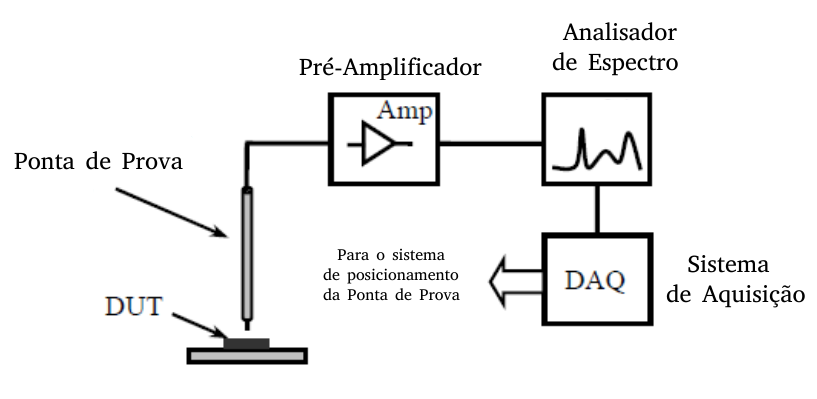
\includegraphics[scale=0.6]{./img/scanning_sistema}
	\fonte{Adaptado de~\citeonline[p.~13]{sivaraman2017}}
	%\legend{\hspace{-218pt}Fonte:~\citeonline[p.~8]{paul2006}}
	\label{fig:scanning}
\end{figure}

O método de varredura, utilizando pontas de provas para detecção de campo eletromagnético próximo é um método geral para identificar a fonte de EMI em circuitos eletrônicos. Vários métodos foram desenvolvidos por muitos autores para o cálculo do padrão de campo distante levando à identificação da fonte do campo. Entretanto, também é necessário conhecer os campos eletromagnéticos em suas características próximas~\apud[p.~17]{sivaraman2017}{gilabert2007}.

% EMC Conuduzida
% EMC Irradiada
% Problematização para detectar o foco do problema em EMC Irradiada

\section{Medidas de Campo Próximo}

As emissões eletromagnéticas irradiadas podem ser medidas em campo próximo ou distante. 

Para a qualificação junto as agencias reguladoras, as medições em campo distante são realizadas, como visto, em 3m e 10m, dependendo da agência. Existe ainda uma serie de procedimentos a serem seguidos, que não serão foco neste trabalho, apenas mencionará-se de forma sucinta que, basicamente, os campos elétricos irradiados para os testes comerciais (FCC e CISPR 22) devem ser medidas em um local de teste de área aberta (\textit{Open-Area Test Site} - OATS) ou em uma câmara semi-anecoica (\textit{Semi Anechoic Chamber} - SAC). Enquanto o OATS é o preferido, o SAC fornece
capacidade de medição em qualquer condição climática, bem como segurança. Uma câmara semi-anecoica é um local blindado com material absorvedor de radiofrequência nas laterais e no topo para evitar reflexões e simular o espaço livre, existem dois propósitos para a câmara semianecoica. O primeiro é evitar que as emissões eletromagnéticas de fora da sala contaminem o teste. A segunda é evitar reflexões nas paredes, de modo a simular o espaço livre, e esse recurso é fornecida pelo material do absorvedor de radiofrequência que reveste as paredes.

As medições realizadas em campo próximo têm como vantagens a precisão, confiabilidade, custo e faixa de aplicação. Em comparação com medições de campo distante, temos que o efeito de alguns fatores incertos, como clima, espalhamento, interferência eletromagnética tem menos influência nas medições de campo próximo porque a sonda e o equipamento sob teste (\textit{Device Under Test} - DUT) estão muito próximos uns dos outros e, portanto, fornecem uma medição mais precisa~\cite{sivaraman2017}.

% O que é Campo Proximo (Near-Field)
% Quais Campos próximos são de interesse aqui

\subsection{Campo Próximo e Campo Distante}
% Diferenças entra os campos próximos e distantes
Para compreendermos melhor as definições temos que o espaço ao redor de uma antena pode ser dividido em três regiões, campo próximo reativo, campo próximo radiativo e campo distante. 

O campo próximo reativo é aquela parte da região do campo próximo imediatamente ao redor
a antena, ou ponta de prova, onde que, para a maioria das antenas, o limite externo desta região é considerado como uma distância $R < 0.62 \sqrt(\frac{D^3}{\lambda})$~\cite[p.~34]{balanis2005}.

O campo próximo radiativo é definido como “aquela região do campo de uma antena entre a região reativa do campo próximo e a região do campo distante e em que a distribuição do campo angular depende da distribuição a partir da antena"~\cite[p.~34]{balanis2005}. Esta região também é conhecida com região de \textit{Fresnel}, fazendo uma analogia com a óptica, esta região é normalmente delimitada por $0.62 \sqrt(\frac{D^3}{\lambda}) < R < 2 \frac{D^2}{\lambda}$

A região de campo distante, ou região de \textit{Fraunhofer} é definida como aquela região do campo de uma antena onde a distribuição angular é independente da distância da antena. Se D é a dimensão global máxima do antena, a região do campo distante está a uma distância maior que  $R > 2 \frac{D^2}{\lambda}$~\cite[p.~16]{sivaraman2017}.

\begin{figure}[htb!]
	\centering 
	\caption{Campos Proximos e Distante}
	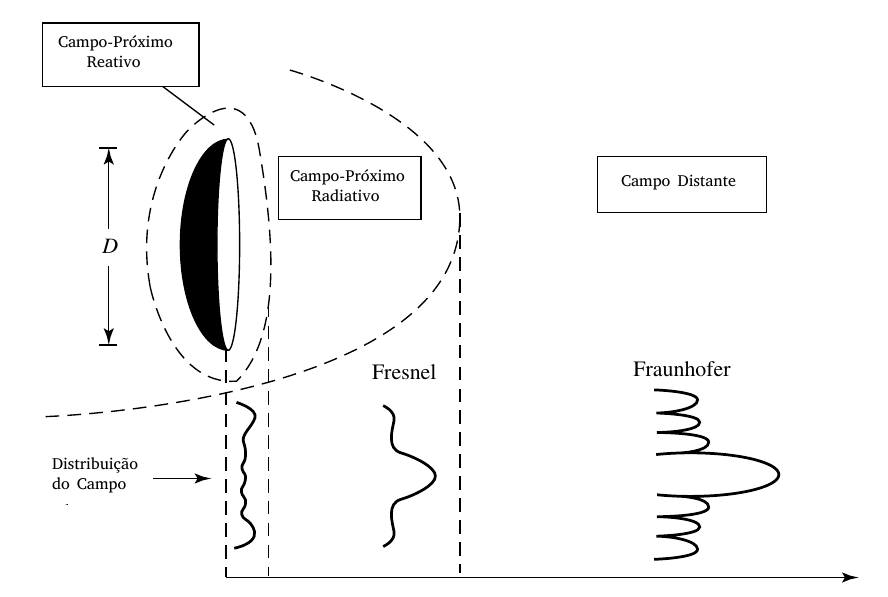
\includegraphics[scale=0.6]{./img/campos_balanis}
	\fonte{Adaptado de~\citeonline[p.~35]{balanis2005}}
	%\legend{\hspace{-218pt}Fonte:~\citeonline[p.~8]{paul2006}}
	\label{fig:regions_campos}
\end{figure}

Na figura~\ref{fig:regions_campos} há descrito as regiões que formam cada tipo de campo, é preciso destacar que as limitações destas regiões são válidas para a condição de $D >\lambda$, vemos também como se comporta a distribuição do campo em cada região.
%To be valid, D must also be large compared to the wavelength (D > λ).

%\subsection{Campo Magnético e Elétrico Próximo}
% Equacionamento Campo Mag e Ele proximos

\section{Pontas de Prova para Campo Próximo}
% Pontas de provas para Campos Proximos
As pontas de provas podem ser aplicadas de duas formas distintas na obtenção de medidas de campo próximo. A primeira configuração é com uma única sonda controlada por um sistema de posicionamento preciso. Na segunda, utiliza-se uma matriz planar de sondas afim de se obter várias medidas simultaneamente. Na figura~\ref{fig:medidas_sondas} visualizamos estas duas diferentes formas de medidas de campo próximo utilizando pontas de provas.

\begin{figure}[htb!]
	\centering 
	\caption{Tipos de medidas de campo próximo}
	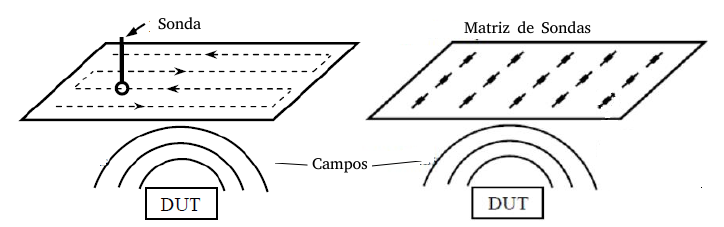
\includegraphics[scale=0.75]{./img/medidas_sondas}
	\fonte{Adaptado de~\citeonline[p.~21]{sivaraman2017}}
	%\legend{\hspace{-218pt}Fonte:~\citeonline[p.~8]{paul2006}}
	\label{fig:medidas_sondas}
\end{figure}

Segundo ~\citeonline[p.~21]{sivaraman2017} a aplicação mais utilizada é na forma de varredura, pois "A presença de um grande número de sondas induz distúrbios de primeira ordem no campo medido".

As pontas de prova de campo próximo (\textit{Near-Field Probe} - NFP) têm sido amplamente estudadas nos últimos anos devido à sua capacidade de quantificar a força do campo próximo (ótico, elétrico ou magnético) no espaço próximo ao sinal fonte. A maioria dos estudos sobre as NFP focou na melhoria da resolução espacial, largura de banda disponível, e suprimindo o campo acoplado em uma direção ortogonal ou campo adverso~\cite[p.~21]{sivaraman2017}. 

% Equacionamento

\subsection{Pontas de Prova Eletro-Ópticas}
% Caracteristicas das pontas eletro-opticas
Um tipo de NFP existente é a eletro-óptica, que consiste em uma sonda que pode ser utilizada para medidas de campos próximos elétricos e magnéticos, tendo como característica a conversão de um sinal eletro-magnético(obtido) para um sinal óptico(transmitido)~\cite[p.~22]{sivaraman2017}.

As ponta de provas ópticas são utilizadas no intuito de eliminar os distúrbios que as sondas metálicas convencionais (eletro-magnéticas) podem provocar no campo original, para isso, nas sondas ópticas há a presença de cristais opto-eletrônicos que convertem os campos medidos em sinais ópticos, não interagindo, de forma significativa, com o campo medido. \citeonline{arakawa2005} analisa a invasividade das sondas ópticas, de forma quantitativa, por simulação utilizando o método de diferenças finitas no domínio do tempo (FDTD). 

\subsection{Pontas de Prova Eletromagnéticas}
% Caracteristicas das pontas Eletromagnéticas
Outro tipo de NFP são as eletromagnéticas, que consistem, em espiras para o caso de detecção do campo magnético próximo, ou de um dipolo para o caso de detecção do campo elétrico próximo, e em ambos os casos, uma linha de transmissão para transportar o sinal induzido~\cite[p.~23]{sivaraman2017}. 

Um desenho comum para uma ponta de prova de campo elétrico consiste em um dipolo e uma linha de transmissão de fios paralelos. Pequenos dipolos são desejáveis ​​porque fornecem alta resolução espacial do campo, e porque permitem uma resposta independente de frequência. Um importante problema associado ao dipolo elétrico é a perturbação imposta ao dispositivo sob teste pela própria sonda~\cite[p.~23]{sivaraman2017}.

Neste trabalho, o foco são as NFP de campo magnético, que basicamente é composta por uma espira que opera de acordo com a lei de \textit{Faraday}

\begin{eqnarray}
\bigtriangledown \times E &=& -\frac{\partial B }{\partial t} \nonumber\\
V_{fem} &=& - \oint_C {E \cdot d\ell = - \frac{d}{{dt}}} \int_S {B_n dA} = -j\omega \mu H_nNA \label{FaradayLaw}
\end{eqnarray}

Onde, $\omega$ é a frequência angular, $\mu$ é a permeabilidade média no centro da espira, $H_n$ é a componente normal do campo magnético, $N$ é o numero de espiras e $A$ a área da espira. 

%Sabendo que: $\omega = 2 \pi f$, $\mu = 4 \pi 10^{-7}$ (no vácuo) e $H$ é a componente normal do campo magnético próximo, dado em $\frac{A}{m}$, temos que a Magnitude da tensão induzida pode ser determinada por:

%\begin{eqnarray}
%| V_{fem} | &=&  0.2 \pi f d^2 H \label{Vfem}
%\end{eqnarray}

A partir da equação~\ref{FaradayLaw} observa-se que a tensão induzida na sonda depende do tamanho da espira (sua área), dessa forma, a sensibilidade da sonda é diretamente proporcional ao tamanho da espira. Sabe-se também, que na sonda contêm não somente a corrente de circulação habitual, induzida pelo campo magnético, mas 
300também correntes que dependem do campo elétrico médio no plano do circuito. Erros grandes podem ser possíveis quando uma
espira é usada para medir campos magnéticos, a menos que seu diâmetro seja menor que $0.01 \lambda$~\cite[p.~25]{sivaraman2017} para não haver polarização do campo elétrico incidente.

Alguns estudos já foram realizados no que tange a fabricação de NFP de campo magnético próximo utilizando PCI. Existem métodos de fabricação de NFPs que vão desde a utilização de filmes finos depositados, tecnologia com semicondutor de metal-óxido complementar (\textit{Complementary Metal Oxide Semiconductor} - CMOS), NFPs integradas em circuitos integrados (CI), porém o foco deste trabalho está na obtenção de NFPs de baixo custo e de fácil fabricação, assim sendo os esforços estarão concentrados nas NFPs confeccionadas em PCIs. ~\citeonline{lin2009} traz o desenvolvimento de uma NFP em PCI com desempenho aprimorado. Na figura~\ref{fig:lin2009} visualizamos a topologia adotada, sendo fabricada sob um substrato de de fibra de vidro (FR4) que possui permissividade $\varepsilon = 4,4$ e espessura $ h = 0,8$mm. As dimensões utilizadas foram R = 4mm e d = 3.5mm e vemos o detalhe quanto ao filtro\textit{microstrip} (entalhes incorporados na linha de transmissão) que funcionam como um filtro para suprimir a auto-ressonância da espira, e, melhorar o desempenho da sonda em freqüências altas~\cite[p.~2]{lin2009}.

\begin{figure}[htb!]
	\centering 
	\caption{NFP com filtro \textit{microsrtip}}
	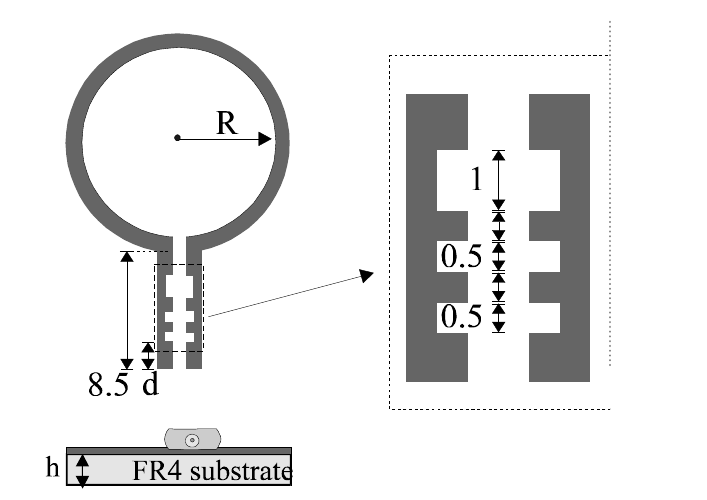
\includegraphics[scale=0.6]{./img/lin2009}
	\fonte{Adaptado de~\citeonline{lin2009}}
	%\legend{\hspace{-218pt}Fonte:~\citeonline[p.~8]{paul2006}}
	\label{fig:lin2009}
\end{figure}

~\citeonline{funato2006} desenvolveu duas topologias, a do tipo A com plano de terra e a do tipo B com uma linha recobrindo a trilha do sinal, na figura~\ref{fig:funato2006} pode-se observar a topologia desenvolvida, em ambas com a linha de transmissão tendo $50\Omega$ com $15$mm de comprimento, com uma espira quadrada contendo $1mm^2$ e confeccionada em FR4 (\textit{Flame Retardant 4} - Designação de classe para material laminado de epóxi reforçado com vidro utilizado em PCI).
\begin{figure}[htb!]
	\centering 
	\caption{NFP com Plano e Linha de Terra}
	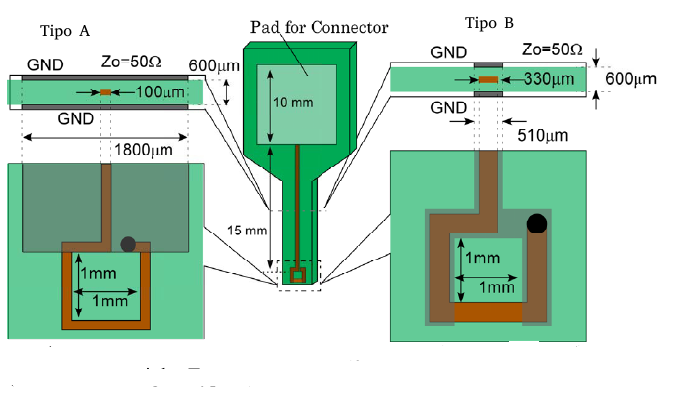
\includegraphics[scale=0.6]{./img/funato2006}
	\fonte{Adaptado de~\citeonline{funato2006}}
	%\legend{\hspace{-218pt}Fonte:~\citeonline[p.~8]{paul2006}}
	\label{fig:funato2006}
\end{figure}


\chapter{Pontas de Prova em análises de compatibilidade eletromagnetica}
% Levantar o historico de utilização de pontas de prova na investigação de EMC em PCIs
Neste capitulo veremos um estudo mais direcionado às características eletromagnéticas e algumas modelagens das NFPs quanto ao seu uso na medição de campo próximo.

Como vimos no capitulo anterior, os valores padronizados pelas agências reguladoras são dados para campo elétrico, porém pode-se realizar as medidas em campo magnético visto que há correlação entre as duas grandezas, e, a partir do campo elétrico obtido por uma conversão de grandeza pode-se comparar com os níveis regulamentados pelas agências. Inicialmente é importante deixar claro alguns conceitos básicos que definem as principais características de uma NFP, vejamos:
% Comentar as Caracteristicas abaixo
%Fatores da Ponta de Prova
\begin{itemize}
 \item \textbf{Fator de Antena}:
 
 O Fator de Antena é definido como a razão entre o campo incidente, ou o campo gerado pelo DUT, sobre a tensão induzida na NFP que está sobre o DUT. O Fator pode ser derivado teoricamente da Lei de Ampere:
 
 \begin{eqnarray}
 AF &=& \frac{1}{j\omega \mu N A} \label{FatorAntena}
 \end{eqnarray}
 
 Onde, $\omega$ é a frequência angular do sinal no DUT, $\mu$ é a permeabilidade magnética, $N$ é o número de espiras e $A$ é a área da espira.

 O Fator de Antena é importante para saber o nível do campo acima do DUT ao usar uma NFP em um sistema de medição de campo próximo. Conforme distancia-se a NFP do DUT, haverá atenuação das irradiações o que influenciará o fator de antena.
 
 \item \textbf{Sensitividade}:
 
 A Sensitividade é definida como a mínima intensidade detectável de um sinal medida pela NFP. A Sensitividade da NFP é diretamente proporcional ao raio da espira, ou ao número de espiras da NFP~\cite[p.~36]{sivaraman2017}.
 
 \item \textbf{Seletividade}:
 
 É a capacidade da NFP de distinguir entre o componente normal e o componente tangencial do campo elétrico ou magnético incidente. A Seletividade de uma NFP é inversamente proporcional ao raio da espira.
 
 \item \textbf{Resolução Espacial}:
 
 O critério de Rayleigh definiu a resolução espacial como a capacidade de uma NFP de distinguir duas fontes com frequências diferentes nas proximidades. Isso equivale a determinar uma distância $\Delta$ da qual a NFP será incapaz de distinguir estas duas fontes.
 
 \item \textbf{Largura de Banda}:
 
 É o intervalo delimitado por uma frequência inferior e outra superior onde a leitura da NFP é constante, podendo ser linearmente constante, ou contantes em valores absolutos.
 
\end{itemize}

A precisão de medições de campo magnético próximo depende muito do tipo de NFP utilizada, como visto a sensibilidade e seletividade da sonda são inversamente proporcionais uma à outra, dessa forma dependendo da topologia de NFP utilizada a medida será ou mais seletiva ou mais sensível. 

\section{Características eletromagnéticas}
% Equacionar as Caracteristicas eletromagneticas
Como viu-se no capitulo anterior, uma NFP de campo magnético consiste basicamente em uma espira e linha de transmissão. Para NFPs de pequenas espiras (raios pequenos) a tensão induzida é determinada pela equação~\ref{FaradayLaw}. 

~\citeonline[p.~1357]{kanda1993} expõe que a partir da equação~\ref{FaradayLaw} pode-se obter a função de transferência de uma NFP de pequenas espiras, sendo que a FT é dada por:

\begin{eqnarray}
FT &=& \left | \frac{V_{fem}}{H_n} \right | = \omega \mu NA    \label{FT_NFP}
\end{eqnarray}

Para que a equação~\ref{FT_NFP} seja válida, temos que necessariamente a NFP seja \textit{eletricamente pequena}. Isso significa que tanto a auto-indutância quanto a capacitância distribuída sejam pequenas e a frequência de operação (banda passante) seja pequena em comparação com a menor frequência de ressonância ($\omega_0 = \frac{1}{\sqrt{LC}}$)~\cite[p.~1357]{kanda1993}.

\subsection{Modelagem do circuito elétrico equivalente}
A ressonância de uma NFP resulta a partir dos valores da capacitância distribuída na espira, a capacitância da linha de transmissão e da auto-indutância da espira. O Circuito elétrico equivalente de uma NFP \textit{eletricamente pequena} pode ser visto na figura~\ref{fig:circuitEQ} 

\begin{figure}[htb!]
	\centering 
	\caption{Circuito Equivalente - NFP \textit{eletricamente pequena}}
	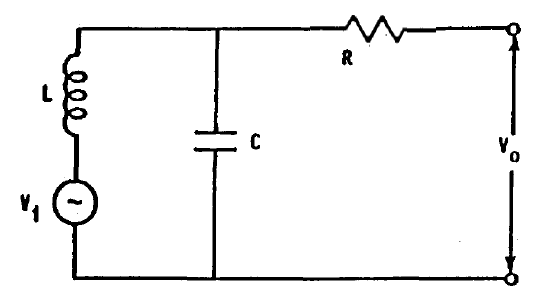
\includegraphics[scale=0.6]{./img/circuitEQ}
	%\fonte{Adaptado de~\citeonline[p.~1358]{kanda1993}}
	\legend{\hspace{-100pt}Fonte: Adaptado de~\citeonline[p.~1358]{kanda1993}}
	\label{fig:circuitEQ}
\end{figure}

Onde, $V_i$ é a tensão induzida (dada pela equação~\ref{FaradayLaw}), $L$ é a auto-indutância, $C$ é a capacitância resultante, e $R$ é a resistência equivalente do circuito (Assumindo que seja independente da frequência) e por fim $V_0$ é a tensão lida sob o circuito. Então a resposta de uma NFP \textit{eletricamente pequena} é dada por:

\begin{eqnarray}
\frac{V_0}{V_i} &=& \frac{-j \frac{1}{\delta }}{\frac{1}{Q} + j \left (\delta - \frac{1}{\delta} \right )} \label{VoVi}
\end{eqnarray}

Onde, $Q = \frac{R}{X_0}$, $X_0 = \omega_0L = \frac{1}{\omega_0C}$, e $\delta = \frac{\omega}{\omega_0}$. Sabendo ainda que $\omega_0 = \frac{1}{\sqrt{L_{i}C_{i}}}$, que é a frequência angular de ressonância, temos que determinar $L$ e $C$, no qual é exposto de forma rigorosa em~\citeonline{kanda1984}, de onde se extrai que:

\begin{eqnarray}
L = \mu b \left \{ln \left ( \frac{8b}{a}  \right ) -2  \right \} \nonumber
\end{eqnarray}

Onde, L é a indutância de uma espira, em que $\mu$ é a permeabilidade do meio, $b$ é o raio da espira, $a$ é o raio do fio que forma a espira. Porém, desde que o raio da espira seja muito maior que o raio do fio, ou seja, $b \gg a$, a indutância $L$ pode ser aproximada por: 

\begin{eqnarray}
L = \mu b ln \left ( \frac{b}{a}  \right )
\end{eqnarray}

~\citeonline{kanda1984} ainda traz que a capacitância da espira pode ser determinada como:

\begin{eqnarray}
C = \frac{2 \epsilon b}{ln \left ( \frac{8b}{a}  \right ) -2 } \nonumber
\end{eqnarray}

Onde, $\epsilon$ é a permissividade do meio que forma a espira. Similarmente ao que ocorre no caso da indutância, se tivermos $ln \frac{b}{a} > 1$, a capacitância da espira pode ser aproximada por:

\begin{eqnarray}
C = \frac{2 \epsilon b}{ln \left ( \frac{b}{a}  \right )}
\end{eqnarray}

Dessa forma, pela equação~\ref{FaradayLaw} que $V_{fem} = V_i  = -j\omega \mu H_nNA$ teremos que a função de transferência de uma espira eletricamente pequena é dada por:

\begin{eqnarray}
FT(f) = \left | \frac{V_0}{H_n} \right | = \omega \mu NA \left | \frac{1}{\frac{1}{Q} + j \left (\delta - \frac{1}{\delta} \right )} \right |
\end{eqnarray}

% Circuito eletromagnetico equivalente
% Equacionamentos
% Tem no funato2006

\subsection{Modelagem como Antena}
% Parametros Fundamentais de Antenas
Uma NFP, além de possuir as características eletromagnéticas expostas anteriormente, também tem propriedades de uma antena do tipo \textit{LOOP} ou circular.

% Loop Antenas
Antenas do tipo \textit{LOOP} podem ser classificadas em duas categorias, eletricamente pequenas e eletricamente grandes. Antenas eletricamente pequenas são aquelas cujo comprimento total (circunferência) é geralmente menor que cerca de um décimo de um comprimento de onda ($C < \lambda / 10$), em contrapartida antenas eletricamente grandes são aqueles cuja circunferência é da ordem do comprimento de onda do espaço livre ($C \sim \lambda $)~\cite[p.~232]{balanis2005}.

\begin{figure}[htb!]
	\centering 
	\caption{Arranjo Geométrico - Análise Antena LOOP}
	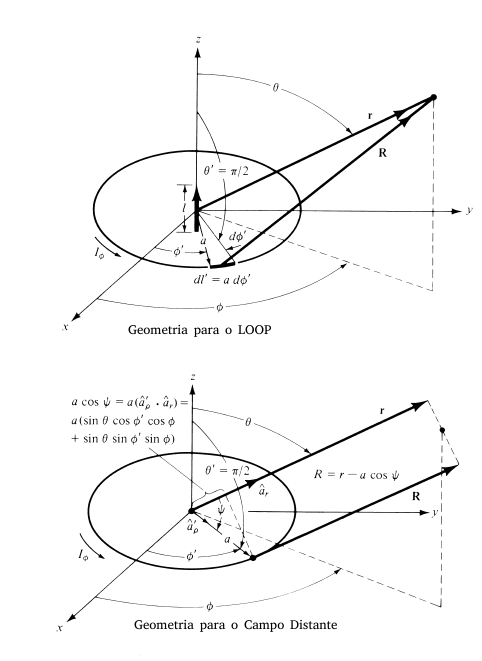
\includegraphics[scale=0.9]{./img/balanis2005_geometria}
	\fonte{Adaptado de~\citeonline[p.~233]{balanis2005}}
	%\legend{\hspace{-100pt}Fonte: Adaptado de~\citeonline[p.~1]{mediano2018}}
	\label{fig:balanis2005_geometria}
\end{figure}

Arranjando geometricamente a antena \textit{LOOP} conforme a figura~\ref{fig:balanis2005_geometria}, ~\citeonline[p.~233]{balanis2005} realizou a análise para obter as componentes do campo magnético e por conseguinte o campo elétrico, sendo que para um \textit{LOOP} pequeno (que pode ser aproximado por um dipolo infinitesimal temos:

\begin{eqnarray}
E_r &=& E_\theta = H_\phi = 0\\
E_\phi &=& -j \frac{k I_m l sin\theta}{4 \pi r} \left [ 1 + \frac{1}{jkr} \right ] e^{-jkr}\\
H_r &=& \frac{I_m l cos\theta}{2\pi \eta r^2} \left [ 1 + \frac{1}{jkr} \right ] e^{-jkr}\\
H_\theta &=& j \frac{k I_m l sin \theta}{4\pi \eta r} \left [ 1 + \frac{1}{jkr} -\frac{1}{(kr)^2} \right ] e^{-jkr}
\end{eqnarray}

Onde, $I_m l = j \omega \mu A I_0$ é o momento de dipolo magnético, sendo $I_0$ a corrente elétrica na espira (nesse caso única).

%A resposta de uma antena, feita de uma espira, é geralmente diretamente proporcional à frequência. Um método para se obter uma resposta plana, em frequência, de uma antena de espira é alterar a impedância da antena com uma resistência de carga no terminal.


\subsection{Grandezas Envolvidas}
Com tudo que vimos até agora, sabemos que os problemas de EMI/EMC estão intimamente relacionados com as correntes no circuito, correntes elétricas operando em altas frequências, sendo estas as responsáveis pelas irradiações nas PCIs, cabos, conectores etc. Devido a este fato, as NFPs, como vimos, são uma ótima ferramenta para identificar essas frequências (sinais). Para isso, comumente se conecta as NFPs em um analisador de espectro para ver as frequências envolvidas no DUT próximo a NFP.~\cite[p.~1]{mediado2018}.

Porém, ainda pode-se surgir a seguinte questão, que grandeza estamos mensurando com a NFP? campo magnético? tensão? ou corrente? Sabe-se que a NFP retorna como informação um valor de tensão elétrica que há de ser aplicado na impedância de entrada do instrumento de medição (Analisador, Osciloscópio, Pré-Amplificado, Filtro, etc.) mas o que exatamente representa este valor de tensão?

\begin{figure}[htb!]
	\centering 
	\caption{Esquema de medidas - Grandezas Envolvidas}
	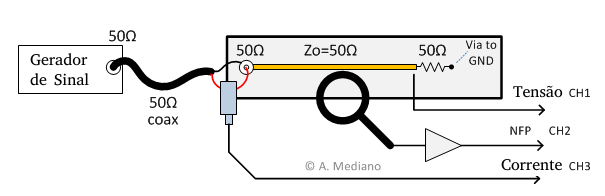
\includegraphics[scale=1]{./img/mediano2018}
	\fonte{Adaptado de~\citeonline[p.~1]{mediado2018}}
	%\legend{\hspace{-100pt}Fonte: Adaptado de~\citeonline[p.~1]{mediano2018}}
	\label{fig:mediano2018}
\end{figure}

Em seu trabalho, ~\citeonline[p.~1]{mediado2018} realizou exatamente esta análise. Na figura~\ref{fig:mediano2018} visualiza-se o esquema de ligação utilizado para investigar quais grandezas estão envolvidas em análises com NFPs, dessa forma ~\citeonline[p.~1]{mediado2018} aplicou sinais senoidais e pulsos quadráticos afim de verificar como se comportam as grandezas envolvidas

\begin{figure}[htb!]
	\centering
 	\caption{Identificação dos Sinais - Grandezas Envolvidas}
	\subfloat[][Sinal Senoidal]{
		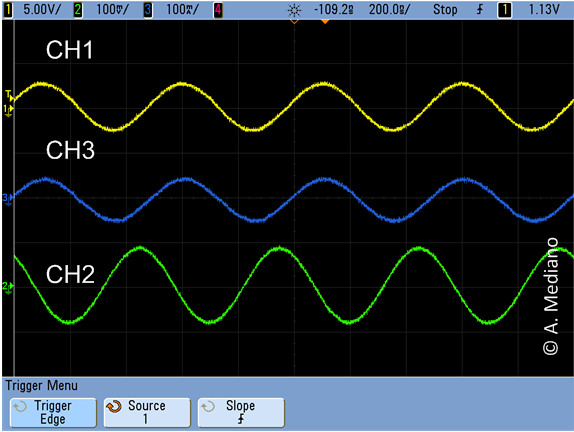
\includegraphics[scale=0.5]{./img/mediado2018_seno}
		\label{fig:mediado2018_seno}}
	\subfloat[][Pulso Quadrático]{
		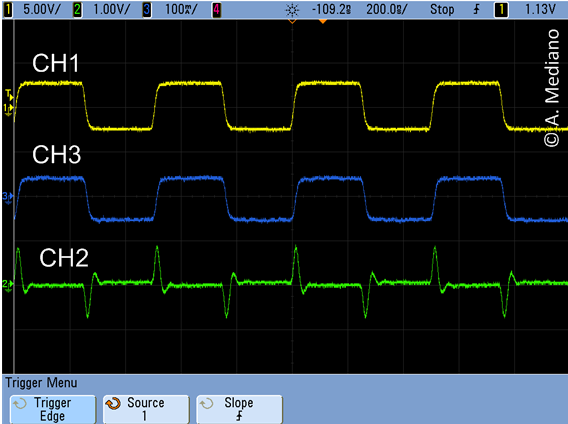
\includegraphics[scale=0.51]{./img/mediano2018_square}
		\label{fig:mediano2018_square}}
    \fonte{Adaptado de~\citeonline[p.~1]{mediado2018}}
\end{figure}

Na figura~\ref{fig:mediado2018_seno}, em seu experimento \citeonline[p.~1]{mediado2018} aplicou no DUT um sinal senoidal de 20MHz, sendo os canais CH1 e CH3 - Tensão e Corrente no DUT, respectivamente, estando estes em fase, devido a termos apenas uma carga puramente resistiva. Porém no canal 2 (CH2), onde esta ligado a NFP, vemos um sinal defasado de $90^{\circ}$. A NFP é sensitiva ao campo magnético, logo a tensão de saída da NFP é proporcional ao campo magnético medido. 

Na figura~\ref{fig:mediano2018_square}, em seu experimento \citeonline[p.~1]{mediado2018} aplicou no DUT um sinal quadrático de 20MHz, notemos agora que o comportamento da NFP é diferente do anterior, haja vista que somente com a variação da corrente $M \frac{\mathrm{d} i}{\mathrm{d} t}$ é que iremos ter variação de fluxo magnético e por conseguinte (Respeitando a lei de Lenz) o aparecimento de uma tensão induzida na espira da NFP.

Diante disto, notemos que, a medida obtida de uma NFP é uma tensão que tem ligação direta com a derivada da corrente no DUT $M \frac{\mathrm{d} i}{\mathrm{d} t}$, sendo $M$ a indutância mútua ou o fator de acoplamento entre a NFP e o DUT.


\chapter{Métodos e Procedimentos}
Neste capítulo será exposto os métodos e procedimentos adotados no desenvolvimento e elaboração dos projetos das NFPs e das medidas realizadas, discorrendo sobre os equipamentos de laboratório necessários à realização das medidas de caracterização e abordando a metodologia utilizada.

\section{Topologias de leiautes desenvolvidas}
A Partir do estudo realizado no capítulo~\ref{fundamentacao} conhecia-se de antemão algumas topologias de leiaute de NFPs, sabia-se, por exemplo, que em regra geral uma NFP para campo magnético próximo, deveria possuir essencialmente duas partes, uma espira (para detecção do campo magnético) e uma linha de transmissão (para conduzir o sinal capturado). Diante deste cenário, estabeleceu-se alguns critérios como: \textbf{(1) a utilização de espiras com raios diferentes, no intuito de verificar a influência do raio (tamanho da espira) na sensibilidade}. \textbf{(2) a verificação da influência do plano de terra na sensibilidade e largura de banda das NFPs} e como último critério \textbf{(3) a adoção de PCIs de face dupla, afim de utilizar 2 espiras (uma em cada face) e verificar a influência do numero de espiras nas características das NFPs}.

Com isso, desenvolveu-se ao todo 20 NFPs separadas em dois grupos, leiautes de face simples e leiautes de face dupla. Para cada grupo destes, utilizou-se cinco tamanhos de raios, 0.5mm, 1mm, 1.5mm, 3mm e 6mm, e para cada raio desenvolveu-se uma NFP com e sem o plano de terra, assim o rol de NFPs desenvolvidas pode ser melhor enumerado da seguinte forma:

\begin{enumerate}
 \item Leiautes de Face Simples:
 \begin{itemize}
  \item FS05ST: Face simples com raio de 0.5 mm sem o plano de terra.
  \item FS05CT: Face simples com raio de 0.5 mm com o plano de terra.
  \item FS10ST: Face simples com raio de 1 mm sem o plano de terra.
  \item FS10CT: Face simples com raio de 1 mm com o plano de terra.
  \item FS15ST: Face simples com raio de 1.5 mm sem o plano de terra.
  \item FS15CT: Face simples com raio de 1.5 mm com o plano de terra.
  \item FS30ST: Face simples com raio de 3 mm sem o plano de terra.
  \item FS30CT: Face simples com raio de 3 mm com o plano de terra.
  \item FS60ST: Face simples com raio de 6 mm sem o plano de terra.
  \item FS60CT: Face simples com raio de 6 mm com o plano de terra.
 \end{itemize}
 
  \item Leiautes de Face Dupla:
 \begin{itemize}
  \item FD05ST: Face dupla com raio de 0.5 mm sem o plano de terra.
  \item FD05CT: Face dupla com raio de 0.5 mm com o plano de terra.
  \item FD10ST: Face dupla com raio de 1 mm sem o plano de terra.
  \item FD10CT: Face dupla com raio de 1 mm com o plano de terra.
  \item FD15ST: Face dupla com raio de 1.5 mm sem o plano de terra.
  \item FD15CT: Face dupla com raio de 1.5 mm com o plano de terra.
  \item FD30ST: Face dupla com raio de 3 mm sem o plano de terra.
  \item FD30CT: Face dupla com raio de 3 mm com o plano de terra.
  \item FD60ST: Face dupla com raio de 6 mm sem o plano de terra.
  \item FD60CT: Face dupla com raio de 6 mm com o plano de terra.
 \end{itemize}
\end{enumerate}

\subsection{Projeto das NFPs}
O leiaute das NFPs foi desenvolvido utilizando o software CAD Altium\textregistered, incluiu-se no circuito uma carga resistiva do tipo SMD (\textit{Surface-Mount Device} - Componente Montado na Superfície) de $50\Omega$ afim de casar impedância com os analisadores de espectro e geradores de funções (Equipamentos utilizados na caracterização).

Na figura~\ref{fig:1A_layers} pode-se visualizar o leiaute desenvolvido para a NFP de face simples com raio de 0.5mm sem o plano de terra. Na figura~\ref{fig:1B_layers} pode-se visualizar o leiaute desenvolvido para a NFP de face simples com raio de 0.5mm com o plano de terra.
\begin{figure}[htb!]
	\centering
 	\caption{NFP face simples - 0.5mm}
	\subfloat[][FS05ST]{
		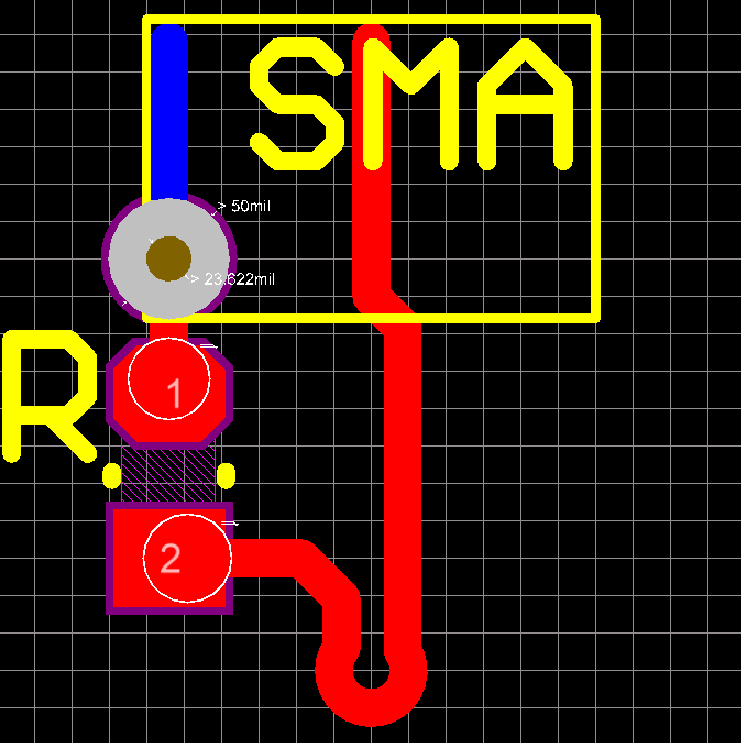
\includegraphics[scale=0.25]{./img/1A_layers}
		\label{fig:1A_layers}}
	\subfloat[][FS05CT]{
		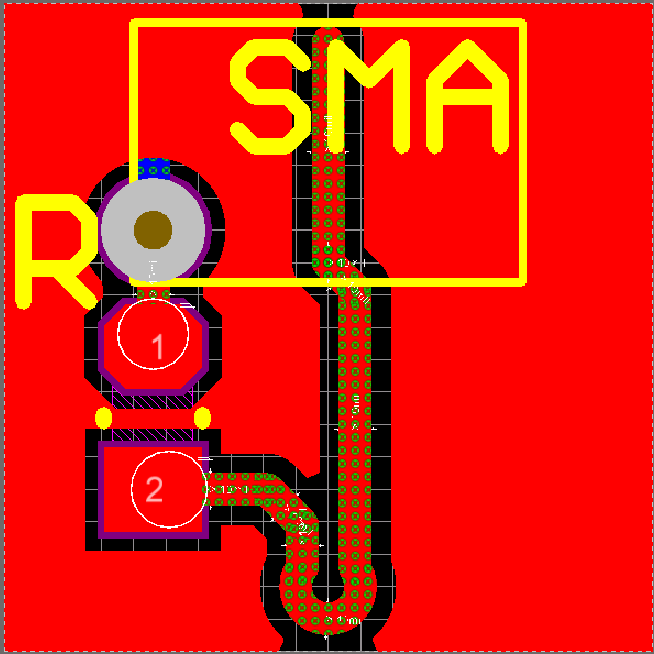
\includegraphics[scale=0.28]{./img/1B_layers}
		\label{fig:1B_layers}}
    \fonte{Elaborado pelo Autor (2019)}
\end{figure}

Na figura~\ref{fig:2A_layers} pode-se visualizar o leiaute desenvolvido para a NFP de face simples com raio de 1mm sem o plano de terra. Na figura~\ref{fig:2B_layers} pode-se visualizar o leiaute desenvolvido para a NFP de face simples com raio de 1mm com o plano de terra.
\begin{figure}[htb!]
	\centering
 	\caption{NFP face simples - 1mm}
	\subfloat[][FS10ST]{
		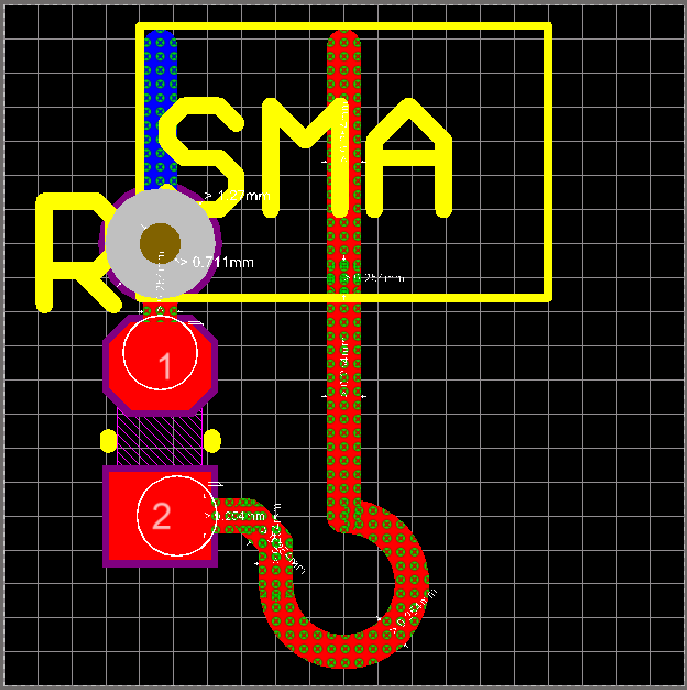
\includegraphics[scale=0.3]{./img/2A_layers}
		\label{fig:2A_layers}}
	\subfloat[][FS10CT]{
		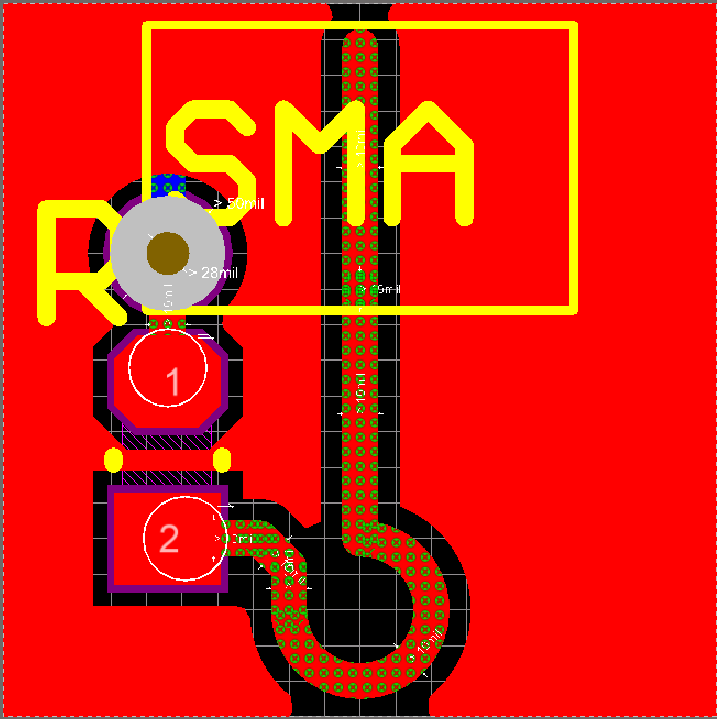
\includegraphics[scale=0.29]{./img/2B_layers}
		\label{fig:2B_layers}}
    \fonte{Elaborado pelo Autor (2019)}
\end{figure}

Na figura~\ref{fig:3A_layers} pode-se visualizar o leiaute desenvolvido para a NFP de face simples com raio de 1.5mm sem o plano de terra. Na figura~\ref{fig:3B_layers} pode-se visualizar o leiaute desenvolvido para a NFP de face simples com raio de 1.5mm com o plano de terra. Como o raios desta NFP ficou 3 vezes maior que as~\ref{fig:1A_layers} e~\ref{fig:1B_layers} notamos que a espira não ficou completa, faltou $\frac{1}{4}$ de volta para realizar a espira completa.
\begin{figure}[htb!]
	\centering
 	\caption{NFP face simples - 1.5mm}
	\subfloat[][FS15ST]{
		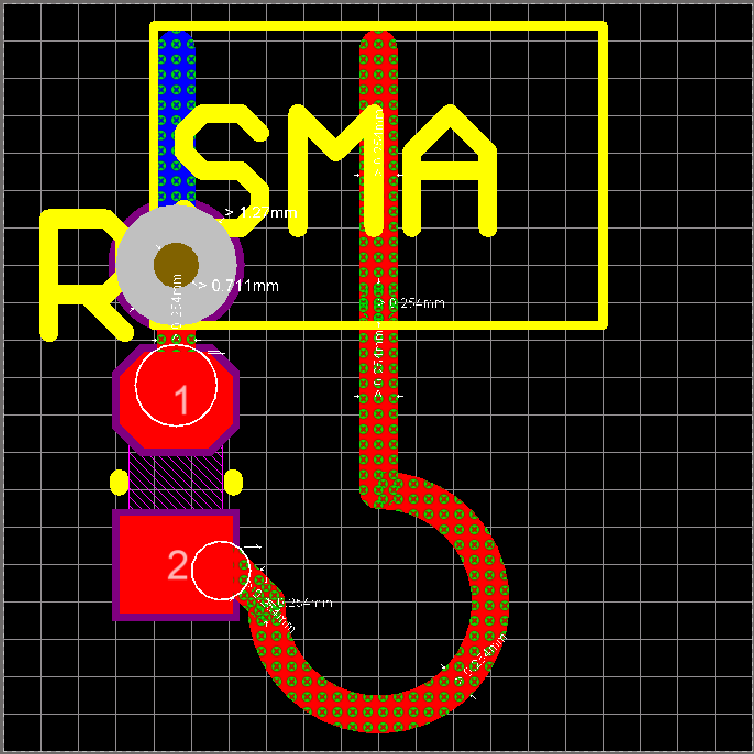
\includegraphics[scale=0.28]{./img/3A_layers}
		\label{fig:3A_layers}}
	\subfloat[][FS15CT]{
		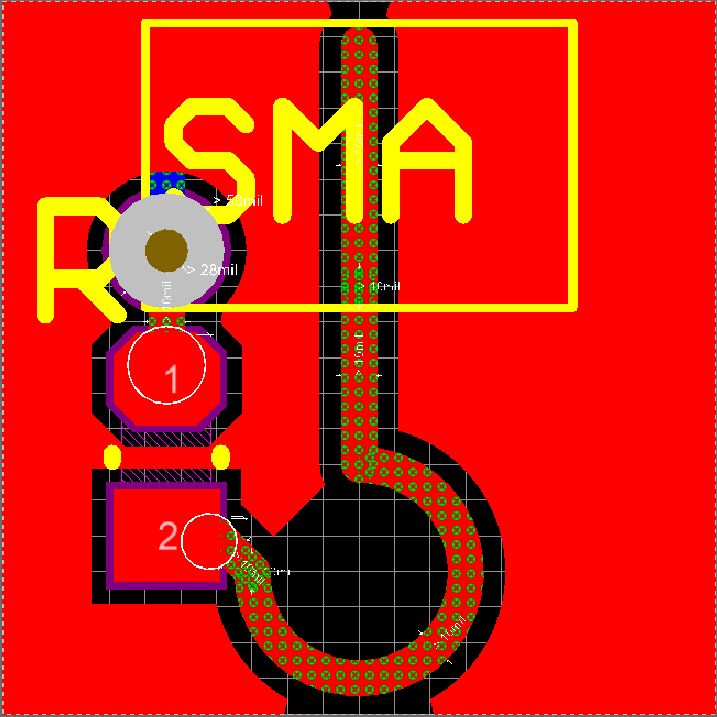
\includegraphics[scale=0.29]{./img/3B_layers}
		\label{fig:3B_layers}}
    \fonte{Elaborado pelo Autor (2019)}
\end{figure}

Na figura~\ref{fig:7A_layers} pode-se visualizar o leiaute desenvolvido para a NFP de face simples com raio de 3mm sem o plano de terra. Na figura~\ref{fig:7B_layers} pode-se visualizar o leiaute desenvolvido para a NFP de face simples com raio de 3mm com o plano de terra. Notamos que nesta NFP a espira ficou quase que completamente fechada.
\begin{figure}[htb!]
	\centering
 	\caption{NFP face simples - 3mm}
	\subfloat[][FS30ST]{
		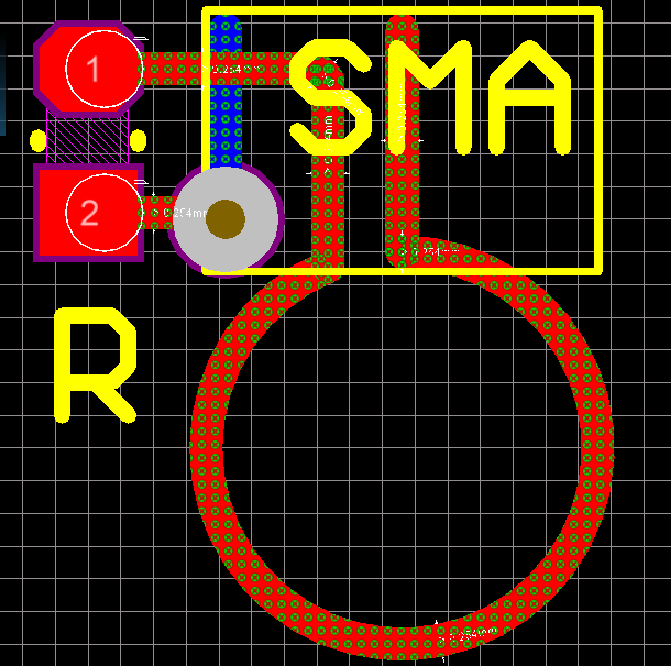
\includegraphics[scale=0.3]{./img/7A_layers}
		\label{fig:7A_layers}}
	\subfloat[][FS30CT]{
		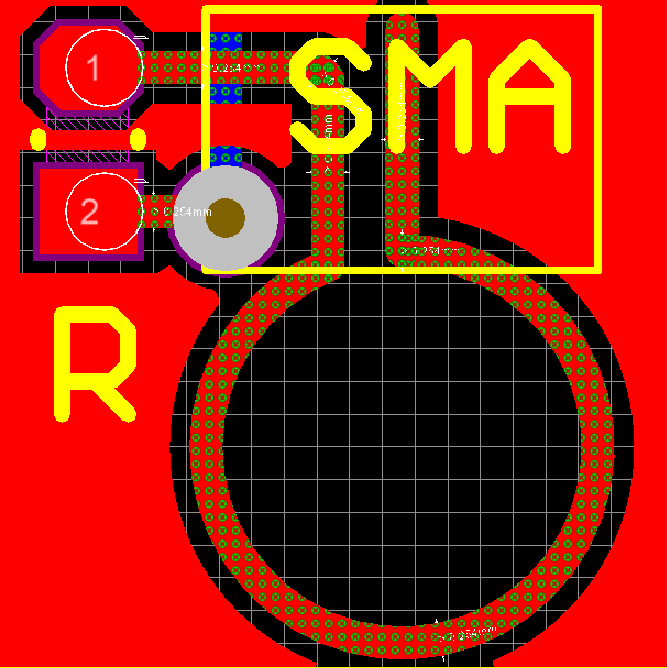
\includegraphics[scale=0.3]{./img/7B_layers}
		\label{fig:7B_layers}}
    \fonte{Elaborado pelo Autor (2019)}
\end{figure}

Na figura~\ref{fig:8A_layers} pode-se visualizar o leiaute desenvolvido para a NFP de face simples com raio de 6mm sem o plano de terra. Na figura~\ref{fig:8B_layers} pode-se visualizar o leiaute desenvolvido para a NFP de face simples com raio de 6mm com o plano de terra. Para esta NFP, devido ao tamanho do raio da espira, foi necessário aumentar as dimensões da PCI, sendo esta a única NFP fora do tamanho adotado como padrão de 10mm por 10mm para as NFPs.
\begin{figure}[htb!]
	\centering
 	\caption{NFP face simples - 6mm}
	\subfloat[][FS60ST]{
		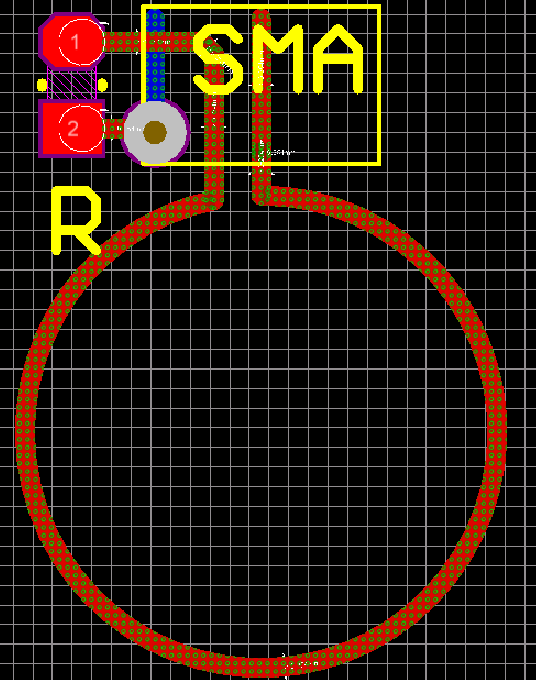
\includegraphics[scale=0.3]{./img/8A_layers}
		\label{fig:8A_layers}}
	\subfloat[][FS60CT]{
		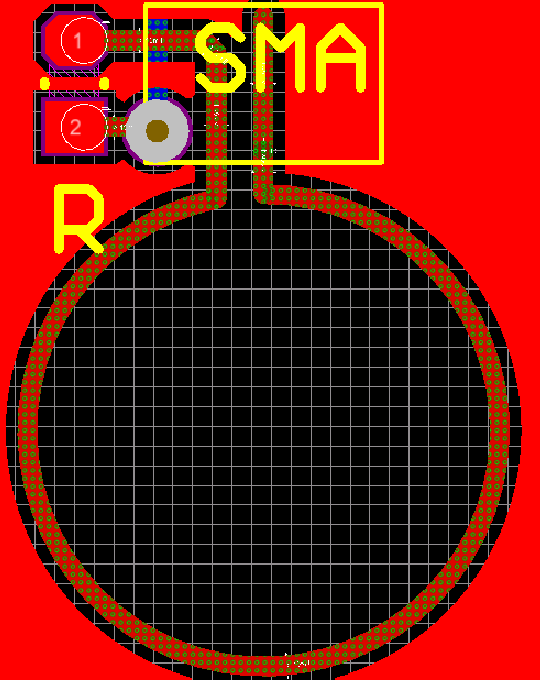
\includegraphics[scale=0.3]{./img/8B_layers}
		\label{fig:8B_layers}}
    \fonte{Elaborado pelo Autor (2019)}
\end{figure}

Desenvolvidas as NFPs de face simples, partiu-se para os leiautes das faces duplas. Na figura~\ref{fig:4A_layers} pode-se visualizar o leiaute desenvolvido para a NFP de face dupla com raio de 0.5mm sem o plano de terra. Na figura~\ref{fig:4B_layers} pode-se visualizar o leiaute desenvolvido para a NFP de face dupla com raio de 0.5mm com o plano de terra. Devido ao fato de necessitar-se de uma via (ligação entre faces) a espira desta NFP assumiu um formato elíptico, preservando-se o menor raio em 0.5mm, no sentido horizontal, porém com uma raio vertical de 2.5mm.
\begin{figure}[htb!]
	\centering
 	\caption{NFP face dupla - 0.5mm}
	\subfloat[][FD05ST]{
		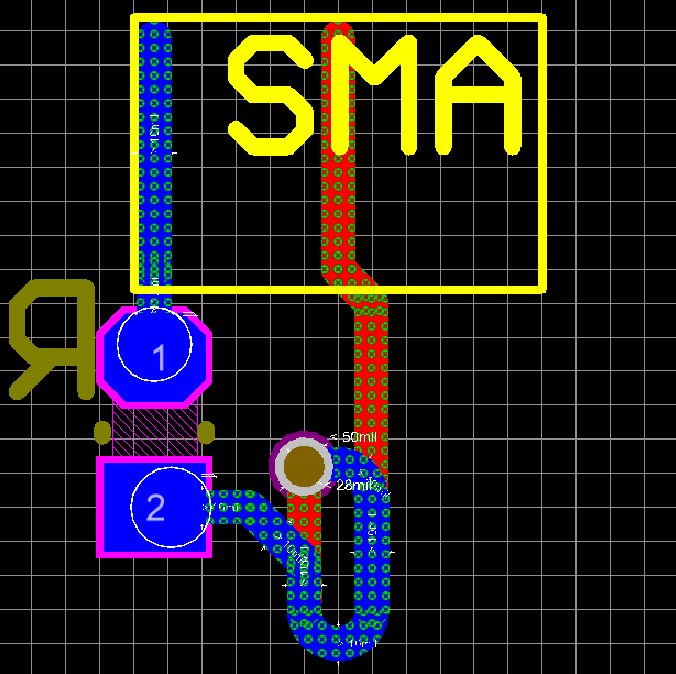
\includegraphics[scale=0.3]{./img/4A_layers}
		\label{fig:4A_layers}}
	\subfloat[][FD05CT]{
		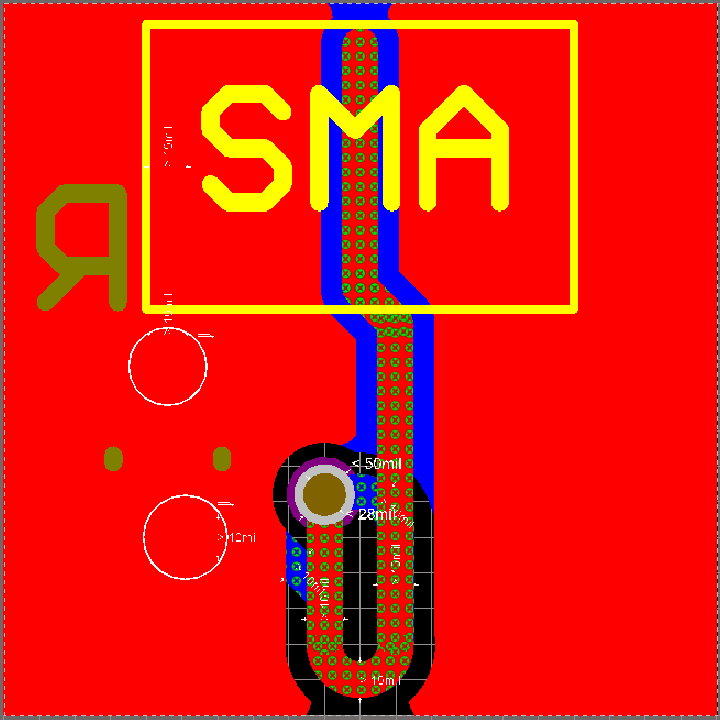
\includegraphics[scale=0.28]{./img/4B_layers}
		\label{fig:4B_layers}}
    \fonte{Elaborado pelo Autor (2019)}
\end{figure}

Na figura~\ref{fig:5A_layers} pode-se visualizar o leiaute desenvolvido para a NFP de face dupla com raio de 1mm sem o plano de terra. Na figura~\ref{fig:5B_layers} pode-se visualizar o leiaute desenvolvido para a NFP de face dupla com raio de 1mm com o plano de terra. 
\begin{figure}[htb!]
	\centering
 	\caption{NFP face dupla - 1mm}
	\subfloat[][FD10ST]{
		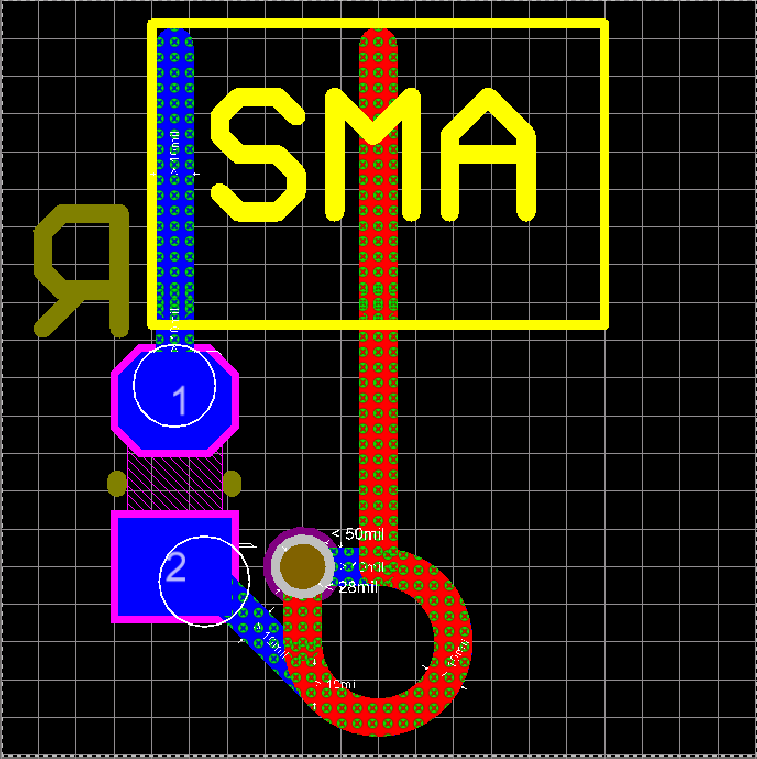
\includegraphics[scale=0.28]{./img/5A_layers}
		\label{fig:5A_layers}}
	\subfloat[][FD10CT]{
		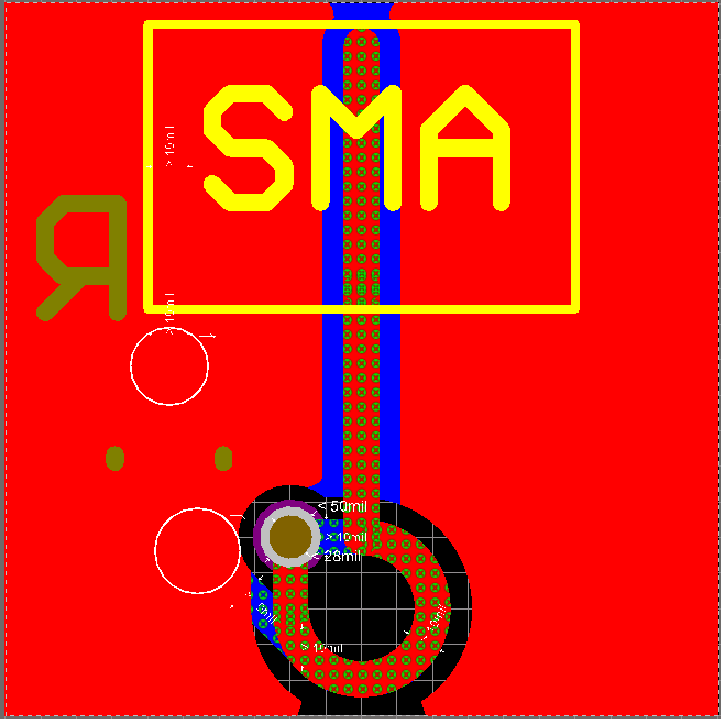
\includegraphics[scale=0.29]{./img/5B_layers}
		\label{fig:5B_layers}}
    \fonte{Elaborado pelo Autor (2019)}
\end{figure}

Na figura~\ref{fig:6A_layers} pode-se visualizar o leiaute desenvolvido para a NFP de face dupla com raio de 1.5mm sem o plano de terra. Na figura~\ref{fig:6B_layers} pode-se visualizar o leiaute desenvolvido para a NFP de face dupla com raio de 1.5mm com o plano de terra. Diferentemente do grupo de face simples, nota-se aqui que as NFPs de face duplas, em pelo menos 1 (uma) espira tem-se a volta completa. 
\begin{figure}[htb!]
	\centering
 	\caption{NFP face dupla - 1.5mm}
	\subfloat[][FD15ST]{
		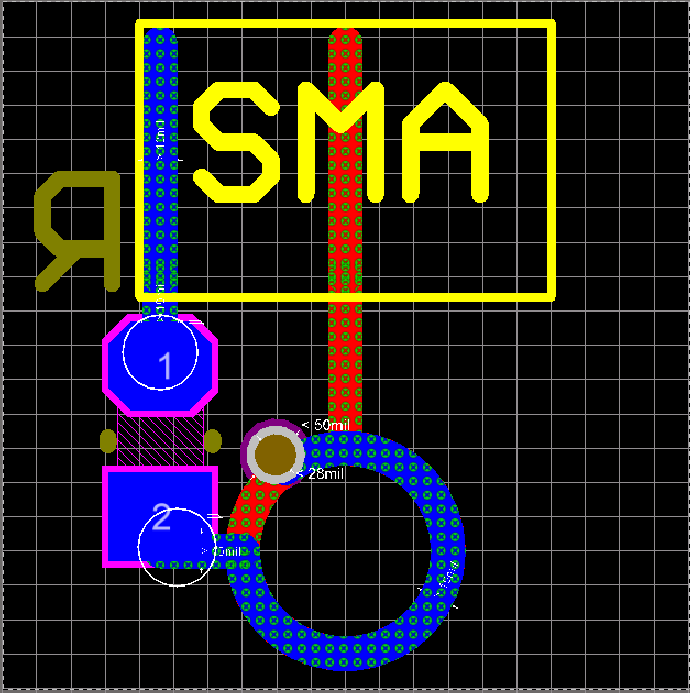
\includegraphics[scale=0.3]{./img/6A_layers}
		\label{fig:6A_layers}}
	\subfloat[][FD15CT]{
		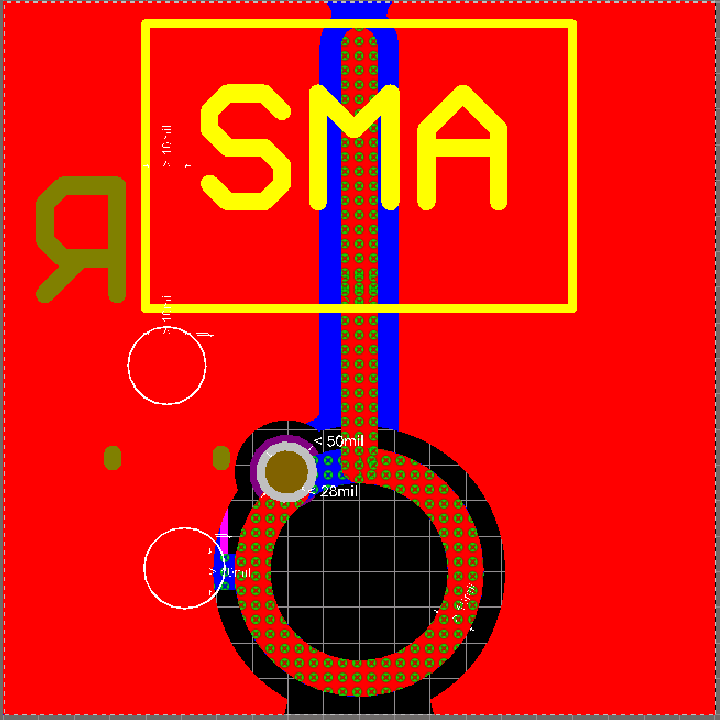
\includegraphics[scale=0.29]{./img/6B_layers}
		\label{fig:6B_layers}}
    \fonte{Elaborado pelo Autor (2019)}
\end{figure}

Na figura~\ref{fig:9A_layers} pode-se visualizar o leiaute desenvolvido para a NFP de face dupla com raio de 3mm sem o plano de terra. Na figura~\ref{fig:9B_layers} pode-se visualizar o leiaute desenvolvido para a NFP de face dupla com raio de 3mm com o plano de terra. 
\begin{figure}[htb!]
	\centering
 	\caption{NFP face dupla - 3mm}
	\subfloat[][FD30ST]{
		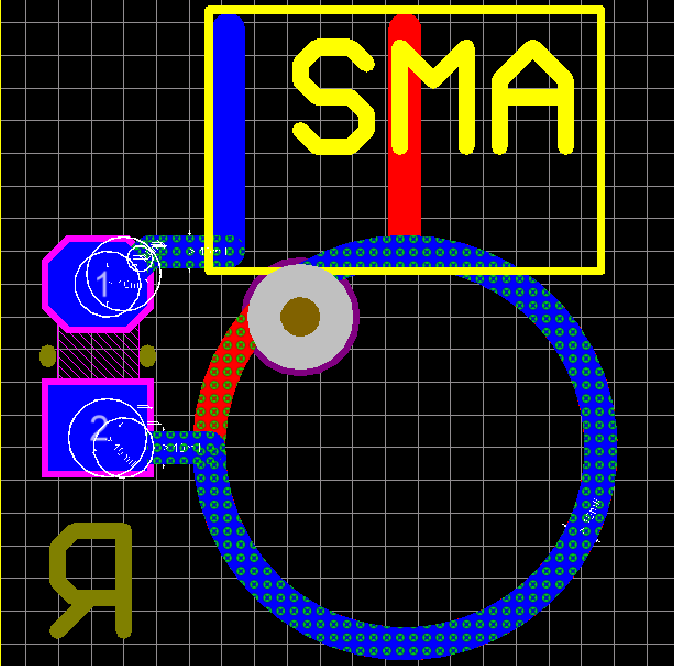
\includegraphics[scale=0.3]{./img/9A_layers}
		\label{fig:9A_layers}}
	\subfloat[][FD30CT]{
		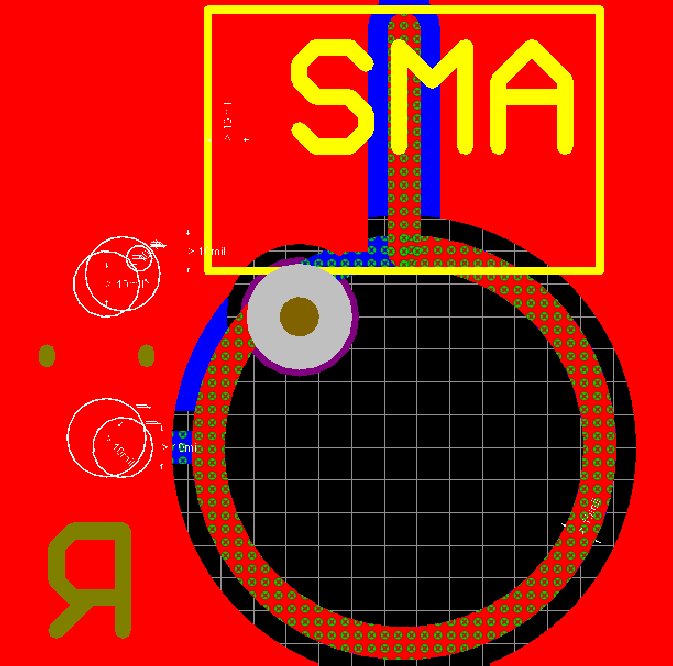
\includegraphics[scale=0.3]{./img/9B_layers}
		\label{fig:9B_layers}}
    \fonte{Elaborado pelo Autor (2019)}
\end{figure}

E por fim, na figura~\ref{fig:10A_layers} pode-se visualizar o leiaute desenvolvido para a NFP de face dupla com raio de 6mm sem o plano de terra. Na figura~\ref{fig:10B_layers} pode-se visualizar o leiaute desenvolvido para a NFP de face dupla com raio de 6mm com o plano de terra. 
\begin{figure}[htb!]
	\centering
 	\caption{NFP face dupla - 6mm}
	\subfloat[][FD60ST]{
		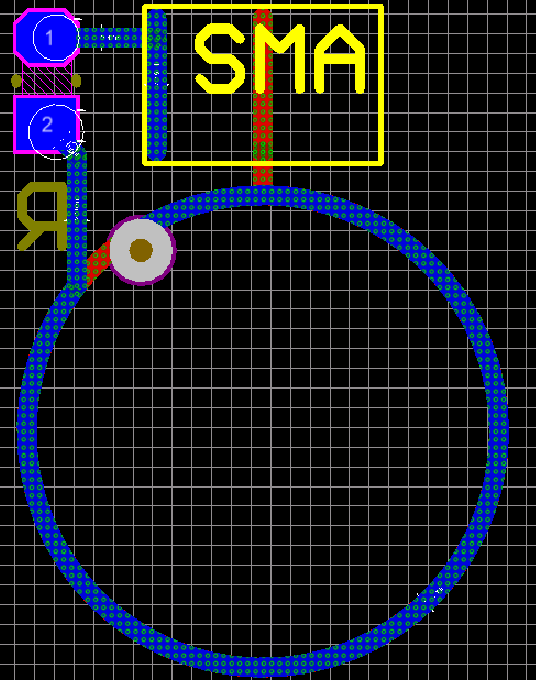
\includegraphics[scale=0.3]{./img/10A_layers}
		\label{fig:10A_layers}}
	\subfloat[][FD60CT]{
		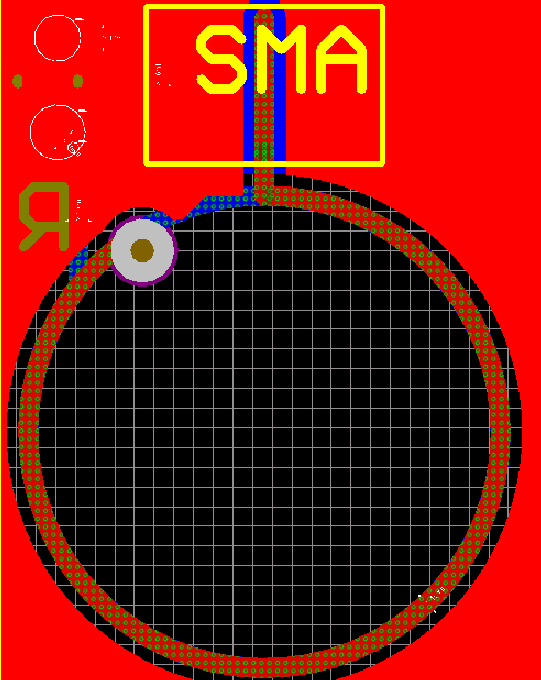
\includegraphics[scale=0.3]{./img/10B_layers}
		\label{fig:10B_layers}}
    \fonte{Elaborado pelo Autor (2019)}
\end{figure}

As maiores dificuldades nos projetos das NFPs, de forma geral, foi a alocação da carga resistiva de $50\Omega$ (Casamento de impedância) e alocar a via (ligação interfaces), esses pequenos empecilhos acarretaram na imperfeição do formato circular, fechado, das espiras, para as NFPs de raios menores que 1.5mm.

% Na figura~\ref{fig:Single_PCI_project} visualiza-se o conjunto de NFPs de face simples preparadas para a fabricação bem como na figura~\ref{fig:Double_PCI_project} visualiza-se o conjunto de NFPs de face dupla também preparadas para a fabricação
% \begin{figure}[htb!]
% 	\centering
%  	\caption{Projeto das NFPs - Fabricação}
% 	\subfloat[][NFPs de Face Simples]{
% 		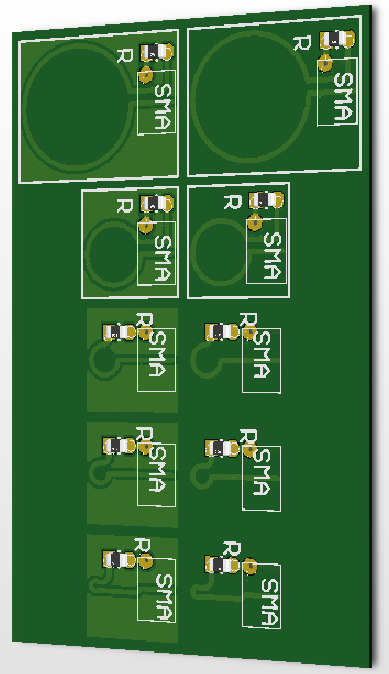
\includegraphics[scale=0.5]{./img/Single_PCI_project}
% 		\label{fig:Single_PCI_project}}
% 	\subfloat[][NFPs de Face Dupla]{
% 		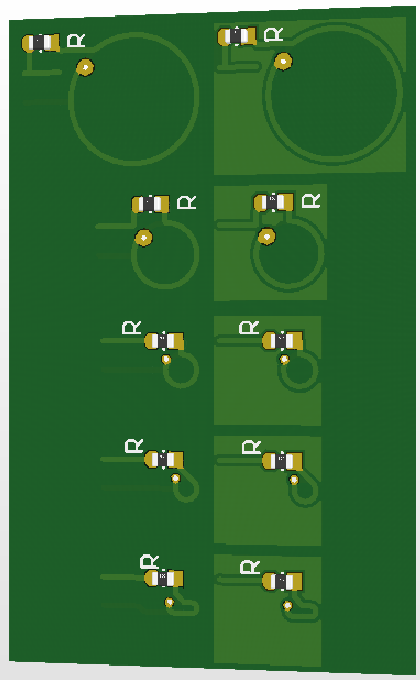
\includegraphics[scale=0.5]{./img/Double_PCI_project}
% 		\label{fig:Double_PCI_project}}
%     \fonte{Elaborado pelo Autor (2019)}
% \end{figure}

\begin{figure}[htb!]
	\centering
 	\caption{NFPs Elaboradas}
	\subfloat[][NFPs de Face Simples]{
		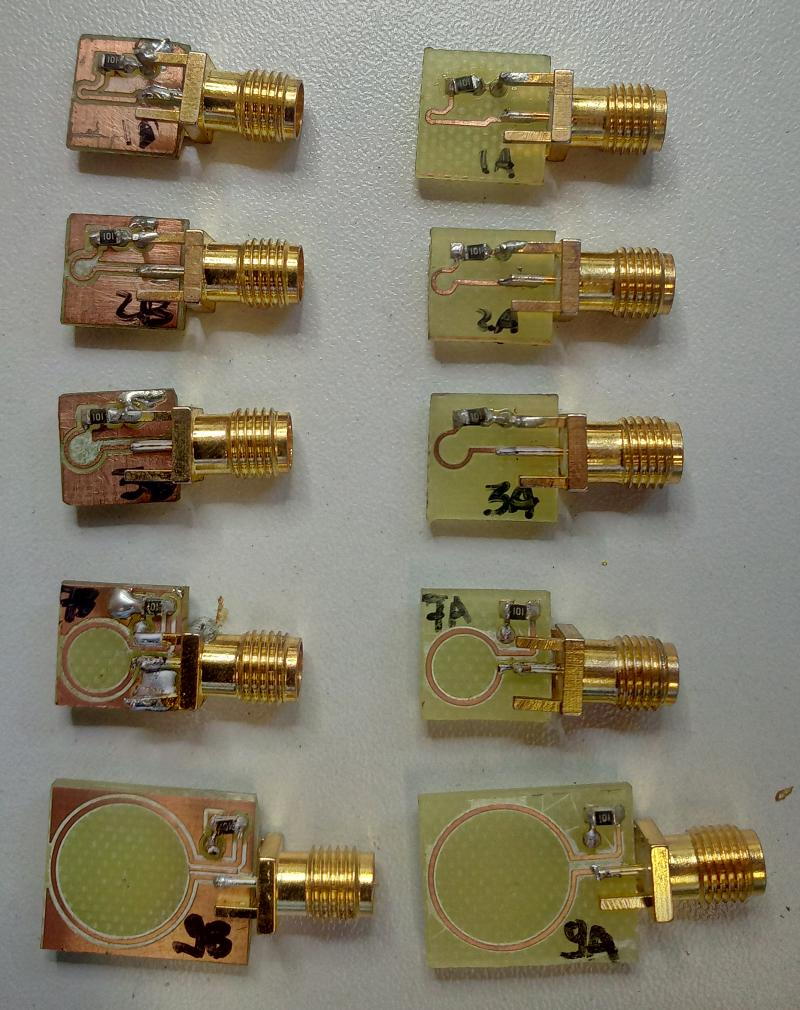
\includegraphics[scale=0.4]{./img/singlefaceNFPS}
		\label{fig:singlefaceNFPS}}
	\subfloat[][NFPs de Face Dupla]{
		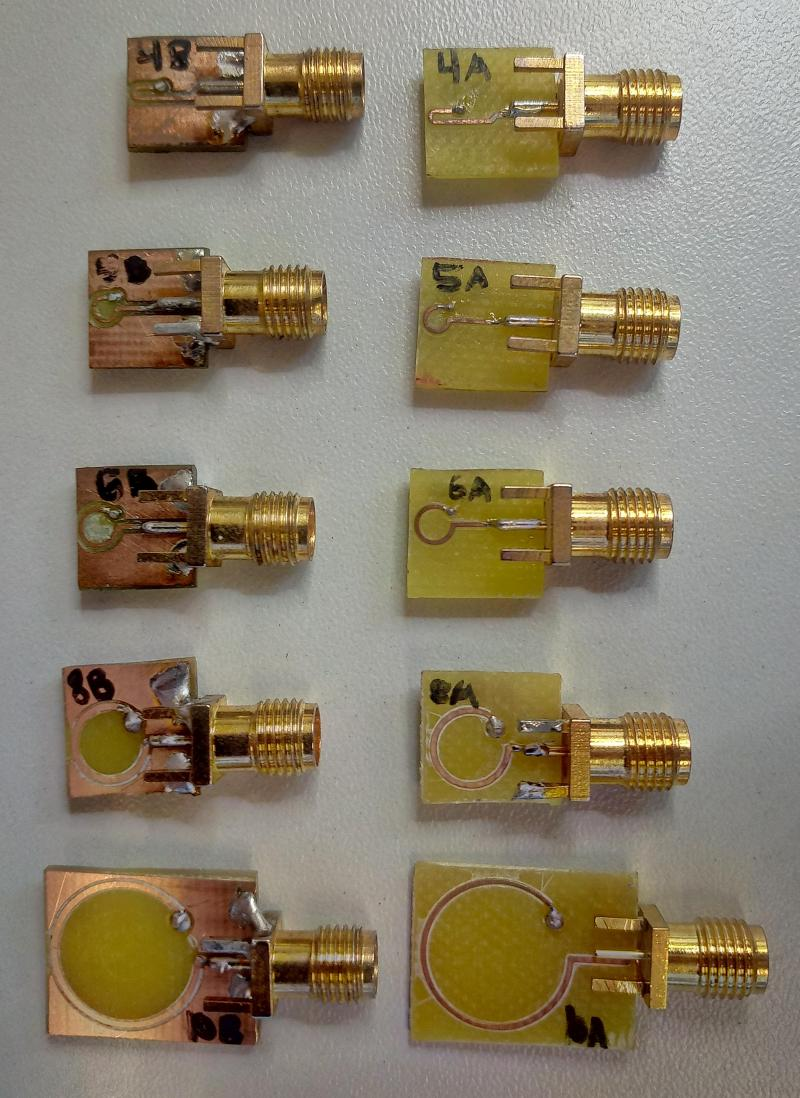
\includegraphics[scale=0.37]{./img/doublefaceNFPS}
		\label{fig:doublefaceNFPS}}
    \fonte{Elaborado pelo Autor (2019)}
\end{figure}

Após a fabricação e montagens o aspecto final das NFPs pode ser visto nas figuras~\ref{fig:singlefaceNFPS} e ~\ref{fig:doublefaceNFPS} de face simples e dupla respectivamente.

\section{Esquemas de medidas e procedimentos}
Para a realização dos experimentos seria necessário, idealmente, ter um sistema de posicionamento XY, porém este sistema de posicionamento será tratado em outro estudo desenvolvido no LabCEM do departamento de eletrônica do IFSC. Assim para realizar as experimentações desenvolveu-se um suporte fixo em madeira (para não interferir nas radiações eletromagnéticas) em que o posicionamento da NFP se deu de forma manual.

\begin{figure}[htb!]
	\centering
 	\caption{Suporte Fixo para posicionamento das NFPs}
	\subfloat[][Visão Superior]{
		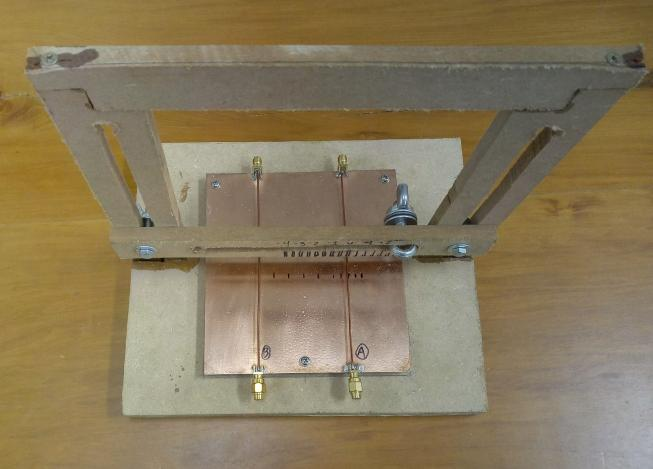
\includegraphics[scale=0.5]{./img/suporteTOP}
		\label{fig:suporteTOP}}
	\subfloat[][Visão Frontal]{
		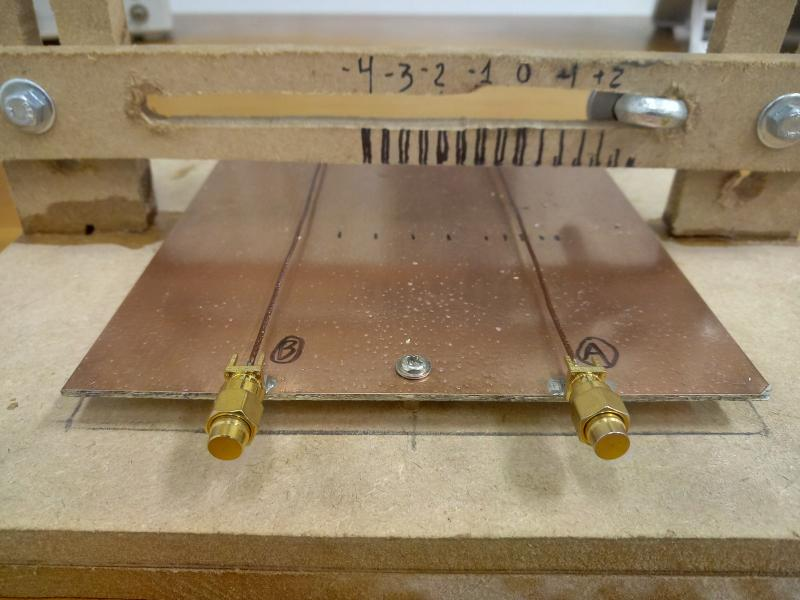
\includegraphics[scale=0.39]{./img/suporteFRONT}
		\label{fig:suporteFRONT}}
    \fonte{Elaborado pelo Autor (2019)}
\end{figure}

Na figura~\ref{fig:suporteTOP} podemos visualizar a vista superior do suporte, onde vemos que o mesmo foi projetado para haver movimentos tanto na direção vertical, onde definiu-se com eixo z, quanto na direção horizontal, definido com eixo y. Vemos também que na base do suporte, em plano fixo, foi alocado o dispositivo sob teste (DUT), mais a frente será detalhado o modelo de DUT utilizado.

Na figura~\ref{fig:suporteFRONT} pode-se visualizar a vista frontal do suporte, onde vemos as marcações para o posicionamento lateral de afastamento, na direção horizontal. Destaca-se aqui que foi adotado o sentido da esquerda para a direita como posições positivas, tomando como referência zero (0mm) o ponto acima do DUT(A), dessa forma, posições mais a direita são valores positivos e posições mais a esquerda são valores negativos.

\subsection{Modelo para o dispositivo sob teste - DUT}
Para implementar um dispositivo sob teste, ou DUT, tomou-se por referência o adotado por~\citeonline[p.~39]{sivaraman2017} porém, para realizar o experimento de caracterização de resolução espacial por DUT duplo, acrescentou-se dois DUTs sob o mesmo plano de terra. Na figura~\ref{fig:esquema3_fundo} visualiza-se os DUTs, que são compostos de dois fios de cobre esmaltados dispostos acima de uma plano de terra, numa distância média de $h = 3mm$, tendo os fios um raio $r = 0,512mm$ ou $18AWG$ separados entre si por uma distância de $D = 60mm$. Em cada fio, numa de suas extremidades esta um conector SMA \textit{SubMiniature version A} - Conector Coaxial de RF de $50\Omega$) e na outra uma carga resistiva de $50\Omega$ ligando o fio ao plano de terra.

\begin{figure}[htb!]
	\centering 
	\caption{Modelo de DUT}
	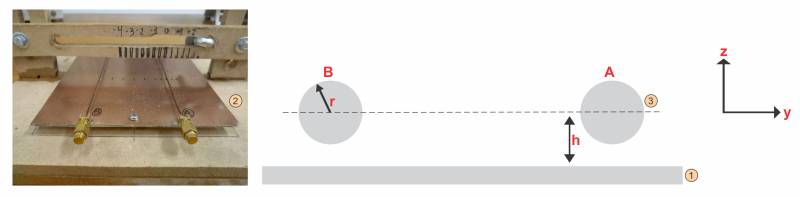
\includegraphics[scale=2.4]{./img/esquema3_fundo}
	\fonte{Elaborado pelo Autor (2019)}
	%\legend{\hspace{-218pt}Fonte:~\citeonline[p.~8]{paul2006}}
	\label{fig:esquema3_fundo}
\end{figure}

Na figura~\ref{fig:esquema3_fundo} vemos marcado em (1) o plano de terra em (2) o DUT real desenvolvido, em (3) o modelo para os fios de cobre esmaltados e ainda vemos uma referência indicativa das direções positivas e eixos adotados nas medições que serão vistas a frente.

%Colocar modelo do circuito elétrico equivalente

\subsection{Equipamentos do laboratório}
Além do suporte e do DUT desenvolvidos, foi necessário a utilização de alguns equipamentos do LabCEM do departamento de eletrônica do IFSC. na figura~\ref{fig:esl} vemos o analisador de espectro da Rohde \& Schwarz modelo ESL3 que foi utilizado para a caracterização da resposta em frequência de 5MHz até 3GHz das NFPs, além da NFP comercial, cujo será realizado uma comparação de performance. Este analisador tem entre as principais características (de interesse para este trabalho) uma faixa de operação de frequência de 9kHz até 3GHz e um gerador de rastreamento com faixa de operação de 1MHz até 3GHz.

\begin{figure}[htb!]
	\centering
 	\caption{Analisadores de Espectro - LabCEM}
	\subfloat[][Analisador ESL]{
		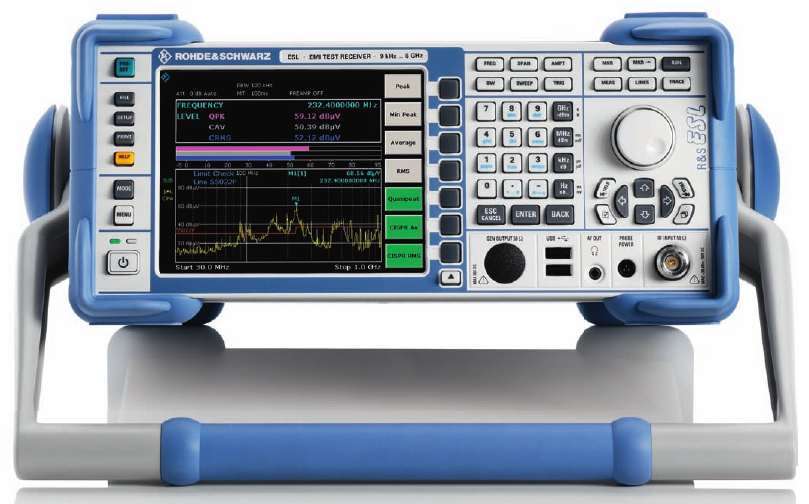
\includegraphics[scale=0.4]{./img/esl}
		\label{fig:esl}}
	\subfloat[][Analisador HMS-X]{
		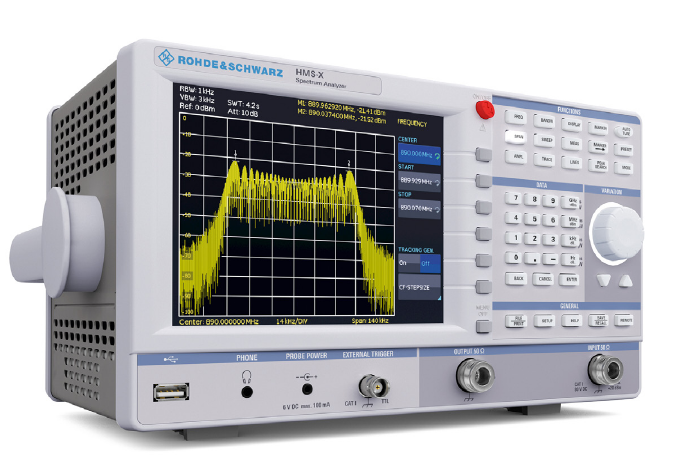
\includegraphics[scale=0.4]{./img/HMS-X}
		\label{fig:HMS-X}}
    \fonte{Elaborado pelo Autor (2019)}
\end{figure}

Outro analisador utilizado é demonstrado na figura~\ref{fig:HMS-X}, também da Rohde \& Schwarz no modelo HMS-X, sendo este utilizado na caracterização em baixas frequências, intensidade por distância e resolução espacial das NFPs com DUT duplo. Este analisador tem entre as principais características (de interesse para este trabalho) uma faixa de operação de frequência de 0Hz até 1.6GHz.

\section{Caracterização da Resposta em Frequência}
O procedimento adotado na caracterização da resposta em frequência consistiu em posicionar cada NFP exatamente sob o DUT(A) (em 0mm, no eixo y) em uma distância de aproximadamente 1mm (eixo z) em relação ao DUT(A), configurou-se o analisador ESL3 para operar no modo gerador de rastreamento (\textit{Tracking generator}), selecionado a frequência inicial em 5MHz e a final em 3GHz, com isso obteve-se a curva de resposta em frequência para cada NFP. Além deste procedimento, também foi realizado a exportação dos dados capturados pelo analisador, afim de realizador um melhor tratamento dos dados via MatLab.

Todas as medidas foram coletadas utilizando a seguinte configuração padrão, RBW = 10kHz, VBW = 100kHz, Ref = 107 $dB \mu V$, tempo de varredura (SWT) = 100ms e Atenuação (Att) = 10dB. Sendo que RBW significa \textit{Resolution Bandwidth} que determina quão próximos dois sinais no domínio da frequência podem ser visualizados. VBW é o \textit{Video Bandwidth} que define a capacidade de discernirem-se dois níveis de potências distintos, uma vez que o sinal digitalizado armazenado pode ser a média de vários pontos próximos.

% Incluir o preset adotado --> RBW; RBW, Ref, sweet, Attenuation, etc...

% Resolução Largura de Banda é uma medida qualitativa da separação mínima necessária entre dois componentes de frequência para poder separá-los visualmente e, para o VSA, é definida como a Largura de Banda de Ruído Equivalente do filtro, que é determinada pelo tipo de janela selecionado e o comprimento da janela.
% 
% Largura de banda de resolução (ResBW ou RBW) afeta o seguinte:
% 
% A resolução de frequência para traços de espectro
% Quão rápido o VSA faz uma medição
% Parâmetro ResBW: especifica o RBW de medição. O VSA ajustará o RBW ao valor mais próximo que satisfaça a configuração de medição atual.
% 
% Como a largura de banda de resolução está diretamente relacionada ao tempo de medição, a seleção manual de uma largura de banda de resolução mais restrita pode atrasar a medição mais do que o necessário. Por outro lado, a seleção de uma largura de banda de resolução muito ampla pode não fornecer a resolução adequada e obscurecer os componentes espectrais que estão próximos uns dos outros.

% 
% O tempo de varredura da tela em um equipamento de medição é afetado por ambas larguras de faixa. Se o VBW for menor que o RBW, o tempo de varredura t_{sweep} é dado por [2]:
% 
% t_{sweep}=\frac{k(f_{2}-f_{1})}{RBW \times VBW}
% 
% onde k é uma constante que depende da construção do equipamento e f2-f1 é a faixa de frequência mostrada na tela.

%Outro procedimento adotado foi a caracterização da resposta em frequência do DUT(A), no intuito de utilizar os dados para anular, via MatLab, o efeito do DUT(A) na respostas das NFPs. 
Também procedeu-se com a caracterização da resposta em frequência de uma NFP comercial, com a intenção de realizar uma comparação com as NFPs produzidas.

\begin{figure}[htb!]
	\centering 
	\caption{Esquema de ligações para medidas - Resposta em Frequência}
	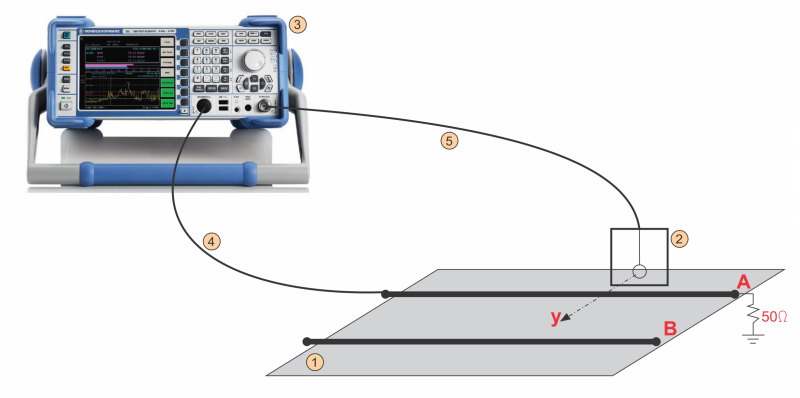
\includegraphics[scale=2.4]{./img/esquema2_fundo}
	\fonte{Elaborado pelo Autor (2019)}
	%\legend{\hspace{-218pt}Fonte:~\citeonline[p.~8]{paul2006}}
	\label{fig:esquema2_fundo}
\end{figure}

Na figura~\ref{fig:esquema2_fundo} pode-se visualizar o esquema de ligação utilizado neste procedimento, onde na marcação (1) temos o plano de terra do DUT(A) e (B), em (2) temos a NFP posicionada, em (3) temos o analisador ESL3, e por fim (4) e (5) vemos os cabos de ligação de saída e entrada respectivamente.

%\subsection{Caracterização da Resposta em Baixas Frequências}
\section{Caracterização da Intensidade por distância}
No intuito de investigar a resolução espacial das NFPs, procedeu-se com a coleta de medidas de intensidade de leitura da NFP pela distância lateral em relação ao DUT, em ~\citeonline[p.~54]{sivaraman2017} adotou-se este procedimento. Como no IFSC não há geradores de funções com capacidade de gerar sinusoides em frequências maiores de que 25MHz, definiu-se por trabalhar na faixa de 5MHz e 25MHz, dentro das possibilidades que os equipamentos disponíveis poderiam entregar.

Para efetuar esta caracterização, na faixa de operação de 5MHz até 25MHz, utilizou-se dois equipamentos, um gerador de função configurado para gerar um sinal sinusoidal de 2Vpp com possibilidade de alterar a frequência na faixa desejada e o analisador de espectro HMS-X capturando a intensidade do sinal obtido na NFP. Foi-se alterando o posicionamento da NFP de 10mm em 10mm em cada direção (positiva e negativa) do eixo y, sendo que em cada posição anotou-se os valores de intensidade $dB\mu V$ para as frequências de 5MHz, 10MHz, 15MHz, 20MHz e 25MHz.

\begin{figure}[htb!]
	\centering 
	\caption{Esquema de Ligações para Medidas - Resposta em Baixas Frequência}
	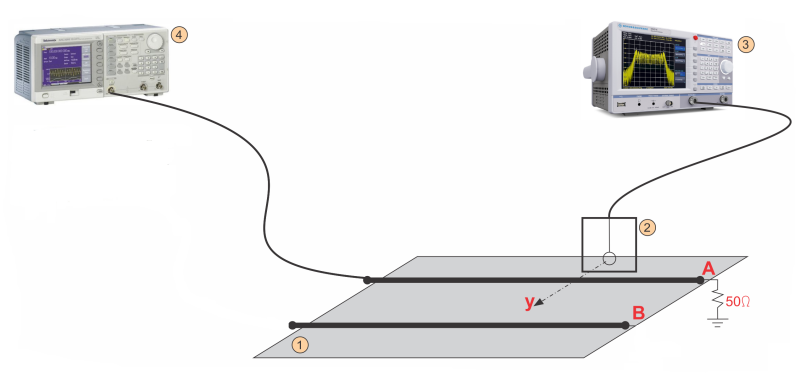
\includegraphics[scale=2.4]{./img/esquema4_fundo}
	\fonte{Elaborado pelo Autor (2019)}
	%\legend{\hspace{-218pt}Fonte:~\citeonline[p.~8]{paul2006}}
	\label{fig:esquema4_fundo}
\end{figure}

Na figura~\ref{fig:esquema4_fundo} pode-se visualizar o esquema de ligação utilizado neste procedimento, onde na marcação (1) temos o plano de terra do DUT(A) e (B), em (2) temos a NFP posicionada, em (3) temos o analisador HMS-X, e por fim em (4) o gerador de função que estará impondo uma senoide de 2Vpp.
%Segunda Leva de Resultados, outra perspectiva da primeira

%Nesta etapa de caracterizações, o procedimento adotado consistiu na utilização do mesmo esquema de montagem visualizado na figura~\ref{fig:esquema4_fundo}, porém foi-se alterando o posicionamento da NFP de 10mm em 10mm em cada direção (positiva e negativa) do eixo y, sendo que em cada posição anotou-se os valores de intensidade $dB\mu V$ para as frequências de 5MHz, 10MHz, 15MHz, 20MHz e 25MHz. Destaca-se que os valores obtidos nessa etapa são os mesmos utilizados na visualização da resposta em frequência, onde ambas as medidas são iguais, apenas utilizou-se perspectivas de análise ou visualização diferentes.

%Primeira Leva de Resultados.

\section{Caracterização da Resolução Espacial - DUT Duplo}
Neste caso, foi necessário a inclusão de um segundo gerador de função, dessa forma teve-se dois DUTs operando simultaneamente, em frequências diferentes, sob o mesmo plano de terra, dessa forma inferiu-se experimentalmente o comportamento de cada NFP em relação a resolução espacial, operando com duas frequências em conjunto. Similarmente as caracterizações anteriores, foi-se alterando o posicionamento da NFP de 10mm em 10mm, porém somente no sentido à esquerda (negativo em y), sendo que em cada posição anotou-se os valores de intensidade $dB\mu V$ para as frequências dos sinais inseridos nos DUTs, sendo que no DUT(A) inseriu-se um sinal sinusoidal de 2Vpp em 20MHz, e no DUT(B) um sinal sinusoidal de 2Vpp em 25MHz

\begin{figure}[htb!]
	\centering 
	\caption{Esquema de Ligações para Medidas - DUT Duplo}
	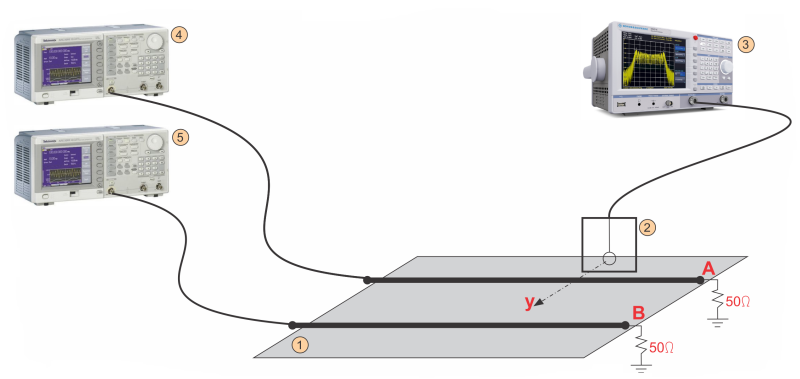
\includegraphics[scale=2.4]{./img/esquema1_fundo}
	\fonte{Elaborado pelo Autor (2019)}
	%\legend{\hspace{-218pt}Fonte:~\citeonline[p.~8]{paul2006}}
	\label{fig:esquema1_fundo}
\end{figure}

Na figura~\ref{fig:esquema1_fundo} pode-se visualizar o esquema de ligação utilizado neste procedimento, onde na marcação (1) temos o plano de terra do DUT(A) e (B), em (2) temos a NFP posicionada, em (3) temos o analisador HMS-X, em (4) o gerador de função que estará impondo uma senoide de 2Vpp de 20MHz no DUT(A) e por fim em (5) o gerador de função que estará impondo uma senoide de 2Vpp de 25MHz no DUT(B).

% \section{Caracterização dos paramentros essencias}
% 
% \subsection{Fator de Antena}
% 
% \subsubsection*{Leiaoutes de face simples}
% 
% \subsubsection*{Leiaoutes de face supla}
% 
% 
% \subsection{Sensitividade}
% 
% \subsubsection*{Leiaoutes de face simples}
% 
% \subsubsection*{Leiaoutes de face supla}
% 
% 
% \subsection{Seletividade}
% 
% \subsubsection*{Leiaoutes de face simples}
% 
% \subsubsection*{Leiaoutes de face supla}
% 
% 
% \subsection{Resolução Especial}
% 
% \subsubsection*{Leiaoutes de face simples}
% 
% \subsubsection*{Leiaoutes de face supla}
% 
% 
% \subsection{Largura de Banda}
% 
% \subsubsection*{Leiaoutes de face simples}
% 
% \subsubsection*{Leiaoutes de face supla}


\chapter{Resultados Experimentais e Discussões}
Neste capítulo serão expostos os resultados das medidas realizadas conforme os métodos e procedimentos elencados no capítulo anterior, será realizado uma descrição do resultado e juntamente será feito uma discussão acerca deste.

\section{Resultados da Caracterização da Resposta em Frequência}
Os gráficos com as respostas em frequência de cada NFP em sua versão com e sem plano de terra esta exposto no apêndice. Neste capítulo deixamos os gráficos que condensam as respostas de todas as NFPs de mesmo tamanho, porém em alguns momentos remeteremos os comentários aos gráficos expostos no apêndice.

\begin{figure}[htb!]
	\centering 
	\caption{Resposta em Frequência - FX05XT}
	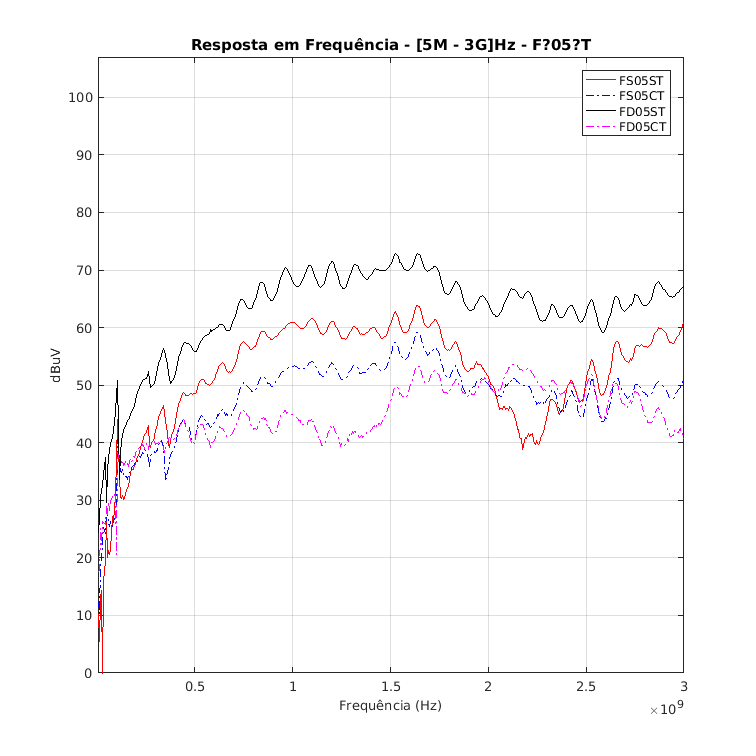
\includegraphics[scale=0.7]{./img/FX05XT}
	\fonte{Elaborado pelo Autor (2019)}
	%\legend{\hspace{-218pt}Fonte:~\citeonline[p.~8]{paul2006}}
	\label{fig:FX05XT}
\end{figure}

Na figura~\ref{fig:FX05XT} visualizamos, de forma condensada, as curvas para a NFP de 0.5mm de raio nas versões em face simples e dupla, com e sem plano de terra (FS05ST, FS05CT, FD05ST e FD05CT respectivamente). Podemos notar inicialmente nesta figura que a NFP na versão face simples sem plano de terra (em vermelho) possui uma região de resposta constante em $dB \mu V$ em uma faixa de frequência que vai de aproximadamente 900MHz à 1.75GHz, enquanto que sua versão face simples com plano de terra (em azul) ocorre um aumento significativo nessa faixa de frequência, em apêndice na figura~\ref{fig:FS05XT} podemos visualizar apenas essas duas curvas. Na versão em face dupla sem o plano de terra (em negro), notamos nitidamente que a sensibilidade em $dB \mu V$ aumenta na ordem de 10 $dB \mu V$, isso se deve ao fato de termos agora dois laços, um em cada face da PCI e novamente notamos (em magenta) que a inclusão do plano de terra, agora em face dupla, suaviza a resposta e aumenta a faixa de frequência que tem uma resposta constante em $dB \mu V$, em apêndice na figura~\ref{fig:FD05XT} podemos visualizar as curvas para as NFPs de face dupla. 

Na figura~\ref{fig:FX10XT} visualizamos, de forma condensada, as curvas para a NFP de 1mm de raio nas versões em face simples e dupla, com e sem plano de terra (FS10ST, FS10CT, FD10ST e FD10CT respectivamente). Podemos notar inicialmente nesta figura que a NFP na versão face simples sem plano de terra (em vermelho) possui uma região de resposta constante em $dB \mu V$ em uma faixa de frequência que vai de aproximadamente 900MHz à 1.75GHz, similar a NFP anterior, nessa versão notamos também que e em 2.2GHz há uma singularidade, %onde $\omega_0 = \frac{1}{\sqrt{L_oC_o}}$ uma ressonância. 
Na versão face simples com plano de terra (em azul) notamos o suprimento dessa singularidade, haja vista que o plano de terra inclui uma capacitância de acoplamento que modifica a resposta do circuito equivalente da NFP. No apêndice na figura~\ref{fig:FS10XT} podemos visualizar apenas essas duas curvas (FS10ST e FS10CT). Na versão em face dupla sem o plano de terra (em negro), notamos um pequeno aumento na sensibilidade, isso se deve ao fato de termos agora dois laços, um em cada face da PCI e novamente notamos (em magenta) que a inclusão do plano de terra, agora em face dupla, suaviza a resposta e aumenta a faixa de frequência que tem uma resposta constante em $dB \mu V$. De todas as versões desta NFP de 1mm, a versão dupla face com plano de terra é a que deu o melhor resultado, mesmo sendo menos sensitiva. Em apêndice na figura~\ref{fig:FD10XT} podemos visualizar as curvas para as NFPs de face dupla.
\begin{figure}[htb!]
	\centering 
	\caption{Resposta em Frequência - FX10XT}
	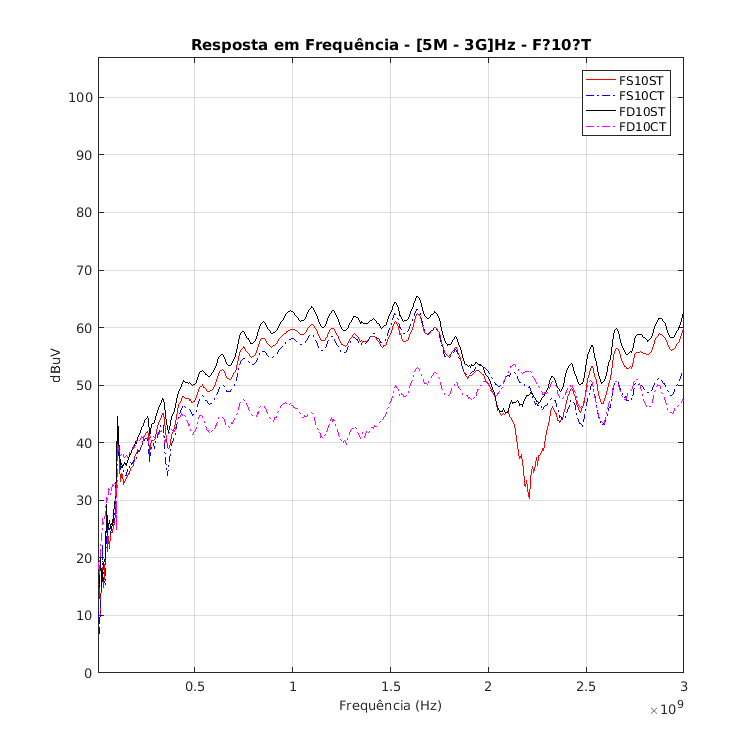
\includegraphics[scale=0.7]{./img/FX10XT}
	\fonte{Elaborado pelo Autor (2019)}
	%\legend{\hspace{-218pt}Fonte:~\citeonline[p.~8]{paul2006}}
	\label{fig:FX10XT}
\end{figure} 

\begin{figure}[htb!]
	\centering 
	\caption{Resposta em Frequência - FX15XT}
	\includegraphics[scale=0.7]{./img/FX15XT}
	\fonte{Elaborado pelo Autor (2019)}
	%\legend{\hspace{-218pt}Fonte:~\citeonline[p.~8]{paul2006}}
	\label{fig:FX15XT}
\end{figure}

Na figura~\ref{fig:FX15XT} visualizamos, de forma condensada, as curvas para a NFP de 1.5mm de raio nas versões em face simples e dupla, com e sem plano de terra (FS15ST, FS15CT, FD15ST e FD15CT respectivamente). Podemos notar inicialmente nesta figura que a NFP na versão face simples sem plano de terra (em vermelho) possui uma região de resposta constante em $dB \mu V$ em uma faixa de frequência que vai de aproximadamente 900MHz à 1.75GHz, mantendo a similaridade com as anteriores. Na versão face simples com plano de terra (em azul) notamos uma aumento significativo da faixa onde há uma resposta constante em $dB \mu V$, haja vista que o plano de terra inclui uma capacitância de acoplamento que modifica a resposta do circuito equivalente da NFP. No apêndice na figura~\ref{fig:FS15XT} podemos visualizar apenas essas duas curvas (FS10ST e FS10CT). Na versão em face dupla sem o plano de terra (em negro), notamos um pequeno aumento na sensibilidade, isso se deve ao fato de termos agora dois laços, um em cada face da PCI, nessa versão notamos mais nitidamente uma singularidade, agora próximo de 2.6GHz e novamente notamos (em magenta) que a inclusão do plano de terra, agora em face dupla, elimina esta singularidade, suaviza a resposta e aumenta a faixa de frequência que tem uma resposta constante em $dB \mu V$. De todas as versões desta NFP de 1.5mm, a versão dupla face com plano de terra é a que deu o melhor resultado, mesmo sendo menos sensitiva. Em apêndice na figura~\ref{fig:FD15XT} podemos visualizar as curvas para as NFPs de face dupla.

\begin{figure}[htb!]
	\centering 
	\caption{Resposta em Frequência - FX30XT}
	\includegraphics[scale=0.7]{./img/FX30XT}
	\fonte{Elaborado pelo Autor (2019)}
	%\legend{\hspace{-218pt}Fonte:~\citeonline[p.~8]{paul2006}}
	\label{fig:FX30XT}
\end{figure}

Na figura~\ref{fig:FX30XT} visualizamos, de forma condensada, as curvas para a NFP de 3mm de raio nas versões em face simples e dupla, com e sem plano de terra (FS30ST, FS30CT, FD30ST e FD30CT respectivamente). Notamos que as versões desta NFP em face simples com e sem plano de terra e face dupla sem plano de terra, apresentam respostas muito similares, possuindo uma região de resposta constante em $dB \mu V$ em uma faixa de frequência que vai de aproximadamente 900MHz à 1.75GHz. Somente na versão face dupla com plano de terra é que notamos uma diferença mais significativo, novamente o plano de terra suavisa a resposta, diminui a sensibilidade porém aumenta a faixa de resposta constante em $dB \mu V$. No apêndice nas figuras~\ref{fig:FS30XT} e ~\ref{fig:FD30XT} podemos visualizar as curvas de forma separada.

\begin{figure}[htb!]
	\centering 
	\caption{Resposta em Frequência - FX60XT}
	\includegraphics[scale=0.7]{./img/FX60XT}
	\fonte{Elaborado pelo Autor (2019)}
	%\legend{\hspace{-218pt}Fonte:~\citeonline[p.~8]{paul2006}}
	\label{fig:FX60XT}
\end{figure}

Na figura~\ref{fig:FX60XT} visualizamos, de forma condensada, as curvas para a NFP de 6mm de raio nas versões em face simples e dupla, com e sem plano de terra (FS60ST, FS60CT, FD60ST e FD60CT respectivamente). Notamos que as versões desta NFP em face simples e dupla sem plano de terra, apresentam respostas muito similares, possuindo uma região de resposta constante em $dB \mu V$ em uma faixa de frequência menor que as anteriores, que vai de aproximadamente 1GHz à 1.5GHz. Nas versões face simples e dupla com plano de terra, notamos que o plano de terra suavisa a resposta, diminui a sensibilidade porém aumenta a faixa de resposta constante em $dB \mu V$. No apêndice nas figuras~\ref{fig:FS60XT} e ~\ref{fig:FD60XT} podemos visualizar as curvas de forma separada.

%###########################
%###########################

\section{Resultados da Caracterização da Intensidade por Distância}
Conforme o procedimento descrito no capítulo anterior, foi coletado para cada posição lateral (na direção do eixo y) o valor de intensidade em $dB \mu V$ nas frequências de 5MHz, 10MHz, 15MHz, 20MHz e 25MHz (limite máximo do gerador de função disponível). Será exposto agora os gráficos contendo o valor de tensão em $dB \mu V$ lido de cada NFP variando-se a posição lateral.

\begin{figure}[htb!]
	\centering
 	\caption{Intensidade por Distância - 5MHz}
	\subfloat[][NFPs Face Simples - 5MHz]{
		\includegraphics[scale=0.4]{./img/FSxxxT_5M}
		\label{fig:FSxxxT_5M}}
	\subfloat[][NFPs Face Dupla - 5MHz]{
		\includegraphics[scale=0.4]{./img/FDxxxT_5M}
		\label{fig:FDxxxT_5M}}
    \fonte{Elaborado pelo Autor (2019)}
\end{figure}

Na figura~\ref{fig:FSxxxT_5M} vemos os gráficos na frequência de 5MHz de todas as versões em face simples, sem e com plano de terra. Nesta imagem, no primeiro quadro, exceto as versões FS30ST e FS60ST, todas as demais tem baixa sensibilidade e pouca resolução espacial, somente as versões FS30ST e FS60ST, que já possuem um raio maior que 1.5mm são as que apresentam uma boa sensibilidade nesta frequência. No segundo quadro da figura~\ref{fig:FSxxxT_5M}, com a inclusão do plano de terra, notamos que todas as versões melhoram sua sensibilidade, e notamos também que a versão FD60CT perde resolução espacial, haja vista que para todas as posições avaliadas esta versão possui um nível de tensão em $dB \mu V$ maior que as demais. 

Na figura~\ref{fig:FDxxxT_5M} vemos os gráficos na frequência de 5MHz de todas as versões em face dupla, sem e com plano de terra. Notamos no primeiro quadro desta imagem que o acréscimo de mais uma volta de espira aumente a sensibilidade para todas as versões de NFPs avaliadas, sendo que a que possui a melhor resolução espacial, nesta frequência é a FD15ST, mesmo sendo a menos sensitiva. No segundo quadro da figura~\ref{fig:FDxxxT_5M} notamos que a inclusão do plano de terra, para esta frequência, não melhora a resolução espacial e não influência de forma significativa a sensibilidade. Dessa forma, o melhor resultado em termos de resolução espacial, nesta frequência (5MHz) é a versão FD15ST.

\begin{figure}[htb!]
	\centering
 	\caption{Intensidade por Distância - 10MHz}
	\subfloat[][NFPs Face Simples - 10MHz]{
		\includegraphics[scale=0.4]{./img/FSxxxT_10M}
		\label{fig:FSxxxT_10M}}
	\subfloat[][NFPs Face Dupla - 10MHz]{
		\includegraphics[scale=0.4]{./img/FDxxxT_10M}
		\label{fig:FDxxxT_10M}}
    \fonte{Elaborado pelo Autor (2019)}
\end{figure}

Na figura~\ref{fig:FSxxxT_10M} vemos os gráficos na frequência de 10MHz de todas as versões em face simples, sem e com plano de terra. Nesta imagem, no primeiro quadro, exceto as versões FS30ST e FS60ST, todas as demais tem baixa sensibilidade e pouco resolução espacial, somente as versões FS30ST e FS60ST, que já possuem um raio maior que 1.5mm são as que apresentam uma boa sensibilidade nesta frequência. No segundo quadro da figura~\ref{fig:FSxxxT_5M}, com a inclusão do plano de terra, notamos que todas as versões melhoram sua sensibilidade, e notamos também que a versão FD60CT perde resolução espacial, haja vista que para todas as posições avaliadas esta versão possui um nível de tensão em $dB \mu V$ maior que as demais. 

Na figura~\ref{fig:FDxxxT_10M} vemos os gráficos na frequência de 10MHz de todas as versões em face dupla, sem e com plano de terra. Notamos no primeiro quadro desta imagem que o acréscimo de mais uma volta de espira aumente a sensibilidade para todas as versões de NFP avaliada, sendo que a que possui a melhor resolução espacial, nesta frequência é a FD15ST, mesmo sendo a menos sensitiva. No segundo quadro da figura~\ref{fig:FDxxxT_5M} notamos que a inclusão do plano de terra, para esta frequência, não melhora a resolução espacial e não influência de forma significativa a sensibilidade. Dessa forma, o melhor resultado em termos de resolução espacial, nesta frequência (10MHz), assim como foi para 5MHZ, é a versão FD15ST.

\begin{figure}[htb!]
	\centering
 	\caption{Intensidade por Distância - 15MHz}
	\subfloat[][NFPs Face Simples - 15MHz]{
		\includegraphics[scale=0.4]{./img/FSxxxT_15M}
		\label{fig:FSxxxT_15M}}
	\subfloat[][NFPs Face Dupla - 15MHz]{
		\includegraphics[scale=0.4]{./img/FDxxxT_15M}
		\label{fig:FDxxxT_15M}}
    \fonte{Elaborado pelo Autor (2019)}
\end{figure}

Na figura~\ref{fig:FSxxxT_15M} vemos os gráficos na frequência de 15MHz de todas as versões em face simples, sem e com plano de terra. Nesta imagem, no primeiro quadro, exceto as versões FS30ST e FS60ST, todas as demais tem baixa sensibilidade e pouca resolução espacial, somente as versões FS30ST e FS60ST, que já possuem um raio maior que 1.5mm são as que apresentam uma boa sensibilidade nesta frequência. No segundo quadro da figura~\ref{fig:FSxxxT_15M}, com a inclusão do plano de terra, notamos que todas as versões melhoram sua sensibilidade, e notamos também que a versão FD60CT perde resolução espacial, haja vista que para todas as posições avaliadas esta versão possui um nível de tensão em $dB \mu V$ maior que as demais. 

Na figura~\ref{fig:FDxxxT_15M} vemos os gráficos na frequência de 15MHz de todas as versões em face dupla, sem e com plano de terra. Notamos no primeiro quadro desta imagem que o acréscimo de mais uma volta de espira aumente a sensibilidade para todas as versões de NFP avaliada, sendo que a que possui a melhor resolução espacial, nesta frequência, continuar sendo a FD15ST, mesmo tendo a menor sensibilidade. No segundo quadro da figura~\ref{fig:FDxxxT_15M} notamos que a inclusão do plano de terra, para esta frequência, não melhora a resolução espacial e não influência de forma significativa a sensibilidade. Dessa forma, o melhor resultado em termos de resolução espacial, nesta frequência (15MHz), assim como foi nas anteriores, é a versão FD15ST.

\begin{figure}[htb!]
	\centering
 	\caption{Intensidade por Distância - 20MHz}
	\subfloat[][NFPs Face Simples - 20MHz]{
		\includegraphics[scale=0.4]{./img/FSxxxT_20M}
		\label{fig:FSxxxT_20M}}
	\subfloat[][NFPs Face Dupla - 20MHz]{
		\includegraphics[scale=0.4]{./img/FDxxxT_20M}
		\label{fig:FDxxxT_20M}}
    \fonte{Elaborado pelo Autor (2019)}
\end{figure}

Na figura~\ref{fig:FSxxxT_20M} vemos os gráficos na frequência de 20MHz de todas as versões em face simples, sem e com plano de terra. Nesta imagem, no primeiro quadro, novamente exceto as versões FS30ST e FS60ST, todas as demais tem baixa sensibilidade e pouca resolução espacial, somente as versões FS30ST e FS60ST, que já possuem um raio maior que 1.5mm são as que apresentam uma boa sensibilidade nesta frequência. No segundo quadro da figura~\ref{fig:FSxxxT_20M}, com a inclusão do plano de terra, notamos que todas as versões melhoram sua sensibilidade, e notamos também que a versão FD60CT perde resolução espacial, haja vista que para todas as posições avaliadas esta versão possui um nível de tensão em $dB \mu V$ maior que as demais. 

Na figura~\ref{fig:FDxxxT_20M} vemos os gráficos na frequência de 20MHz de todas as versões em face dupla, sem e com plano de terra. Notamos no primeiro quadro desta imagem que o acréscimo de mais uma volta de espira aumente a sensibilidade para todas as versões de NFP avaliada, sendo que a que possui a melhor resolução espacial, nesta frequência, continuar sendo a FD15ST, mesmo tendo a menor sensibilidade. No segundo quadro da figura~\ref{fig:FDxxxT_20M} notamos que a inclusão do plano de terra, para esta frequência, não melhora a resolução espacial e não influência de forma significativa a sensibilidade. Dessa forma, o melhor resultado em termos de resolução espacial, nesta frequência (20MHz), assim como foi nas anteriores, é a versão FD15ST.

\begin{figure}[htb!]
	\centering
 	\caption{Intensidade por Distância - 25MHz}
	\subfloat[][NFPs Face Simples - 25MHz]{
		\includegraphics[scale=0.4]{./img/FSxxxT_25M}
		\label{fig:FSxxxT_25M}}
	\subfloat[][NFPs Face Dupla - 25MHz]{
		\includegraphics[scale=0.4]{./img/FDxxxT_25M}
		\label{fig:FDxxxT_25M}}
    \fonte{Elaborado pelo Autor (2019)}
\end{figure}

Na figura~\ref{fig:FSxxxT_25M} vemos os gráficos na frequência de 25MHz de todas as versões em face simples, sem e com plano de terra. Nesta imagem, no primeiro quadro, novamente exceto as versões FS30ST e FS60ST, todas as demais tem baixa sensibilidade e pouca resolução espacial, somente as versões FS30ST e FS60ST, que já possuem um raio maior que 1.5mm são as que apresentam uma boa sensibilidade nesta frequência. No segundo quadro da figura~\ref{fig:FSxxxT_25M}, com a inclusão do plano de terra, notamos que todas as versões melhoram sua sensibilidade, e notamos também que a versão FD60CT perde resolução espacial, haja vista que para todas as posições avaliadas esta versão possui um nível de tensão em $dB \mu V$ maior que as demais. 

Por fim, na figura~\ref{fig:FDxxxT_25M} vemos os gráficos na frequência de 25MHz de todas as versões em face dupla, sem e com plano de terra. Notamos no primeiro quadro desta imagem que o acréscimo de mais uma volta de espira aumente a sensibilidade para todas as versões de NFP avaliada, sendo que a que possui a melhor resolução espacial, nesta frequência, continuar sendo a FD15ST, mesmo tendo a menor sensibilidade. No segundo quadro da figura~\ref{fig:FDxxxT_25M} notamos que a inclusão do plano de terra, para esta frequência, não melhora a resolução espacial e não influência de forma significativa a sensibilidade. Dessa forma, o melhor resultado em termos de resolução espacial, nesta frequência (25MHz), assim como foi nas anteriores, é a versão FD15ST.

%###########################
%###########################

\section{Resultados da Caracterização da Resolução Espacial}
Conforme o procedimento descrito no capítulo anterior, realizou-se a captura da intensidade de tensão na NFP em $dB \mu V$ agora com dois DUTs operando simultaneamente, afim de verificar a distinção de cada frequência em posições espaciais diferentes. Estes resultados nos trazem uma melhor noção de resolução espacial e distinção de diferentes frequências.

\begin{figure}[htb!]
	\centering 
	\caption{Intensidades por Distâncias - NFPs Face Simples}
	\includegraphics[scale=0.45]{./img/DUTDuplo_FS}
	\fonte{Elaborado pelo Autor (2019)}
	%\legend{\hspace{-218pt}Fonte:~\citeonline[p.~8]{paul2006}}
	\label{fig:DUTDuplo_FS}
\end{figure}

Na figura~\ref{fig:DUTDuplo_FS} visualizamos as medidas coletadas para todas as versões face simples, sendo que nos quadros da primeira fileira visualizamos as versões sem plano de terra e na fileira inferior visualizamos as versões com plano de terra. No primeiro quadro visualizamos as medidas coletadas para a NFP FS05ST e logo abaixo sua versão com plano de terra FS05CT, notamos que ambas as versões possuem respostas similares quanto a resolução espacial e distinção das frequências. No quadro que mostra a NFP FS30CT notamos uma leve diferenciação das frequências, porém é no caso FS60ST apresenta a melhor resolução espacial, porém em todas as posições são lidos valores mais altos de tensão em $dB \mu V$ do que as demais NFPs, mostrando que esta NFP é mais sensitiva do que as demais.

\begin{figure}[htb!]
	\centering 
	\caption{Intensidades por Distâncias - NFPs Face Simples}
	\includegraphics[scale=0.45]{./img/DUTDuplo_FD}
	\fonte{Elaborado pelo Autor (2019)}
	%\legend{\hspace{-218pt}Fonte:~\citeonline[p.~8]{paul2006}}
	\label{fig:DUTDuplo_FD}
\end{figure}

Na figura~\ref{fig:DUTDuplo_FD} visualizamos as medidas coletadas para todas as versões face dupla, sendo que nos quadros da primeira fileira visualizamos as versões sem plano de terra e na fileira inferior visualizamos as versões com plano de terra. No primeiro quadro visualizamos as medidas coletadas para a NFP FD05ST e logo abaixo sua versão com plano de terra FD05CT, aqui ja notamos uma boa resolução espacial para a FD05ST - lembramos aqui que esta NFP é a versão que ficou em um formato elíptico, isso pode ter influenciado neste resultado. Outra evidência clara que notamos é no quadro da FD15ST, que confirma que esta NFP tem uma boa resolução espacial, ficando assim de acordo com as medidas efetuadas na caracterização da intensidade por distância, exposta na última seção deste capítulo. Notamos também que as versões FD60ST e FD60CT também apresentam uma boa resolução espacial, porém estas NFPs são mais sensitivas que as demais, fornecendo valores de tensão em $dB \mu V$ em todas as posições avaliadas.

%###########################
%###########################

%\section{Melhores Resultados}


\chapter{Aplicações, Considerações Finais e Conclusão}
Neste capítulo será discorrido acerca de algumas possibilidade de aplicações de NFP, encerrando com as principais conclusões que puderam ser extraídas deste trabalho bem como as considerações para trabalhos futuros que possam a vir ser realizados no âmbito do LabCEM do IFSC - Engenharia Eletrônica.

\section{Aplicações}
\subsection{Medidas de campo próximo}
A principal utilidade das NFPs esta na detecção de campo próximo afim de se efetuar análises de compatibilidade eletromagnética. Após a identificação de alguma frequência que esteja fora dos padrões e limites exigidos pelas normas, ou que interfira em algum tipo de susceptibilidade, muitas vezes se faz necessário rastrear no circuito a origem deste sinal espúrio, para isso existe o método de rastreamento utilizando uma NFP. 

Vimos nesse estudo que as NFPs desenvolvidas aqui em PCI, obtiveram excelentes resultados na detecção de frequências entre 5MHz até 25MHz (limites impostos pelos equipamentos disponíveis) para a verificação ponto a ponto, e, via analisador de espectro, viu-se que na faixa de 900MHz até 1.5GHz, temos uma resposta plana das NFPs desenvolvidas. Portanto, as NFPs desenvolvidas são viáveis a serem aplicadas na detecção de sinais espúrios via rastreamento por varredura.

\subsubsection{Produto Comercial}
Uma aplicação viável que foi vislumbrada durante a realização deste trabalho, foi quanto a prática comercial das NFPs desenvolvidas, dessa forma realizou-se uma comparação de resultados entre as características de resposta em frequência de uma NFP que está disponível comercialmente e algumas NFPs desenvolvidas neste trabalho. Na figura~\ref{fig:FD15CTeCOM} visualizamos as repostas para as versões FD15CT, FD30CT, FD60CT e uma NFP comercial, e notamos claramente que as NFPs desenvolvidas aqui possuem respostas tão boas quanto a NFP comercial investigada.

\begin{figure}[htb!]
	\centering 
	\caption{Resposta em Frequência - FD15CT, FD30CT, FD60CT e Comercial}
	\includegraphics[scale=0.7]{./img/FD15CTeCOM}
	\fonte{Elaborado pelo Autor (2019)}
	%\legend{\hspace{-218pt}Fonte:~\citeonline[p.~8]{paul2006}}
	\label{fig:FD15CTeCOM}
\end{figure}

Diante deste fato, concluímos que as NFPs desenvolvidas em PCI são viáveis até para serem comercialmente trabalhadas, sendo que o preço de fabricação em PCI é mínimo. A título também de comparação buscou-se o valor praticado comercialmente na venda de pontas de prova de campo próximo e descobriu-se que frente ao custo de 1 conector SMA, 1 placa PCI de 10mm x 10mm e algumas horas trabalhadas (custo das NFPs aqui desenvolvidas) o preço comercial de NFPs em PCI daria uma margem de lucro muito alta. Na figura~\ref{fig:NFP_comercial_price} vemos que um kit com 4 NFP custa a monta de 295,00 (Duzentos e Noventa e cinco Dolares) o que equivale aproximadamente à 1150 (Mil Cento e Cinquenta Reais). Na figura~\ref{fig:NFP_comercial_meansure} visualizamos a NFP comercial investigada.

\begin{figure}[htb!]
	\centering
 	\caption{Preços e Medida - NFP Comercial}
	\subfloat[][Preço - NFP Comercial]{
		\includegraphics[scale=0.4]{./img/NFP_comercial_price}
		\label{fig:NFP_comercial_price}}
	\subfloat[][Medida - NFP Comercial]{
		\includegraphics[scale=0.4]{./img/NFP_comercial_meansure}
		\label{fig:NFP_comercial_meansure}}
    \fonte{Elaborado pelo Autor (2019)}
\end{figure}

\subsection{Inserção de Campo Magnético}
Além de detectar, as NFPs são antenas e pelo principio da dualidade de antenas, as NFPs aqui desenvolvidas podem também serem aplicadas na inserção de campos magnéticos, no intuito de averiguar se a frequência do sinal inserido provoca algum tipo de anomalia ou defeito no DUT avaliado. Esta ação pode ser realizada juntamente com uma varredura, efetuando assim uma análise de compatibilidade eletromagnética do DUT e identificando a susceptibilidade ou não deste DUT à algum sinal espúrio que por ventura possa provocar defeitos.

%\subsubsection{Neuro Iteração}

\section{Considerações Finais}

\subsection{Aprimoramentos e Melhorias Necessárias}
% Sistema de medida precisa ser melhorado.. Necessário maior confiança no posicionamento.
Um dos principais pontos de melhorias é em relação ao sistema de posicionamento da NFP. Neste trabalho, conforme apresentado, utilizou-se um aparato em madeira cujo posicionamento foi feito manualmente, isso acarreta em erros de posicionamento e aumenta significativamente o tempo de medição. Sendo assim, seria de grande relevância para o LabCEM o desenvolvimento de um sistema automatizado de posicionamento das NFPs juntamente com um sistema eletrônico para aquisição dos dados.

Quanto aos leiautes desenvolvidos, poderia-se melhorar a disposição da carga resistiva e das vias de ligações entre uma face e outra (para as versões em face dupla), principalmente nas versões de NFP com raios pequenos (0.5mm, 1mm e 1.5mm). Isto seria possível utilizando métodos de fabricação de PCI comerciais com limites de \textit{clearance}, furação e trilhas mais sofisticados do que os disponíveis no IFSC, apesar do IFSC possuir ferramentas de fresa e métodos muito bons de fabricação de PCI, os limites são restritivos ao projetista, impondo certos limites de liberdade à escolha de um melhor posicionamento destes componentes.

\subsection{Dificuldades e Problemas Encontrados}
Uma das primeiras dificuldades encontradas foi na etapa de desenvolvimento e projeto das NFPs. As versões em face dupla necessitaram de uma via (interligação entre faces) além da carga resistiva para o casamento de impedância, e com isso, principalmente nos leiautes com raio menor que 1.5mm, teve-se dificuldades em alocar a via e projetar as espiras com volta completa. O caso de destaque aqui foram as versões FD05ST e FD05CT, cujo espira ficou no formato elíptico, isso acarretou em um comportamento levemente diferenciado em relação as demais.

% Equipamentos do LabCEM são Excelentes... mas na bibliografia utiliza-se muito um analisador de rede
Outra dificuldade, não tão impactantes, foi quanto ao uso de gerador de função e analisadores de espectro em falta de analisador de rede vetorial. Apesar de o LabCEM possuir excelentes equipamentos, nas referências adotadas é utilizando o analisador de rede vetorial nas caracterizações de intensidade por distância. O uso deste equipamento possibilitaria uma investigação em uma faixa muito maior de frequências e possibilitaria também algum tipo de investigação mais aprofundada quanto a ganhos e funções de transferências das NFPs desenvolvidas.

% Dificuldade para gerar frequências maiores que 25 MHz ... Geradores do IFSC vão no máximo a esta frequência
Por fim, apesar de termos apresentado a caracterização da resposta em frequência em uma faixa larga de 5MHz à 3GHz, nas investigações de intensidade por distância ficou-se limitado à máxima frequência disponível nos geradores de função dos laboratórios do IFSC, estabeleceu-se como faixa de investigação de 5MHz a 25MHz (limite máximo em frequência dos gerados disponíveis), isso não prejudicou o trabalho, porém uma análise mais ampla, principalmente na faixa de resposta plana das NFPs, não foi possível de se realizar.

\subsection{Perspectivas Futuras}
% Outras Topologias, Elipticas e Quadradas
O estudo e investigação realizada neste trabalho, não esgota as possibilidades de novas intervenções afim de cada vez mais esclarecer e entender o comportamento e resultados das pontas de prova de campo próximo. Um estudo que poderia ser realizado consequente a esse é quanto a utilização de outros formatos de topologias, como viu-se em dos casos aqui utilizou-se uma topologia elíptica (FD05ST e FD05CT) e esta apresentou em um resultado diferenciado em relação as outras, então, seria de grande valia um novo estudo e investigação quanto a diferentes topologias de espiras, como a elíptica e a quadrada.

% Modelagem matematica de um modelo de NFP.
Outro trabalho que poderia ser consequente a este, e um nível mais elevado e aprofundado, seria uma modelagem matemática com um equacionamento preciso da resposta e comportamentos de alguma topologia de ponta de prova de campo próximo, este trabalho estaria na vanguarda desta área e poderia trazer a tona uma equação precisa para projetos de NFPs.

% Software para simular medida em campo próximo.
Também caberia no futuro a elaboração de algorítimos que se propusessem a simular o comportamento e resultados de pontas de prova de campo próximo, afim de obter-se previamente resultados de simulação e assim confronta-los com resultados práticos coletados por sistemas de varredura automatizados.

% Estudar o custo de fabricação, desenvolvimento e a prática comercial destas NFPs... Montar um plano de negócios
Por fim, caberia também um estudo comercial de custos de fabricação e elaboração de algum plano de negócios quanto a exploração comercial destas NFPs, haja vista, como vimos, há hoje no mercado pontas de prova de campo próximo sendo comercializadas apenas no exterior (fora do Brasil) que entregam resultados similares aos obtidos com as pontas de prova em PCI aqui desenvolvidas.
	
\section{Conclusão}
%Estudar, Desenvolver e investigar experimentalmente topologias em placas de circuito impresso para sondas de campo próximo que sejam eficientes e de baixo custo para a obtenção de medidas de campo magnético próximo em análises de compatibilidade eletromagnética.

% Fator Antena
% Sensitividade
% Seletividade
% Resolução Espacial
% Largura de Banda

% Influência do Raio na Sensitividade
% Influência do plano de terra na sensibilidade e largura de banda
% 2 espiras na sensibilidade

%+ Espiras --> ++Sensitividade
%+ Plano de terra elimina ressonâncias, Diminui a Sensitividade (na banda passante) porém melhora a banda passante
%+ Para Raios grandes +Espiras não aumentam significativamente a sensibilidade
Através dos resultados obtidos na caracterização da resposta em frequência, podemos concluir que o número de espiras influencia diretamente na sensibilidade das NFPs, aumentando-a, algo previamente esperado conforme revisado no capítulo de fundamentação teórica e modelagem eletromagnética. Além disso, podemos verificar que a adição de um plano de terra insere uma capacitância de acoplamento ao terra que melhora significativamente a largura de banda para uma resposta plana em $dB \mu V$ das NFPs, porém, em contrapartida esse plano de terra diminui a sensibilidade. Por fim, nesta caracterização, notamos que o aumento do raio da espira também melhora a sensibilidade nos casos em que aumentamos de raios pequenos (0.5mm) para raios médios (1.5mm), porém para a situação de dobrar o raio de 3mm para 6mm não trouxe um aumento significativo na sensibilidade.

%Intensidade por distância
%+ Para Raios grandes temos boa sensibilidade, porém com o aumento da frequência diminui-se a resolução espacial, com plano de terra, diminui-se a resolução espacial (raios grandes)
%+ Raios grandes são bons para sensibilidade
Com os resultados obtidos na caracterização das intensidades pela distância, podemos notar, dentro da faixa analisada de 5MHz até 25MHz, que as NFPs de raios grandes (3mm e 6mm) possuem uma boa sensibilidade em toda a faixa analisada, porém aumentando-se a frequência perdemos a resolução espacial, pois começa-se a ter leituras altas de intensidade para posições cada vez mais afastadas, dessa forma, concluímos que NFPs com raios grandes são excelentes em sensibilidade porém perdem resolução espacial.

%    5MHz --> FD15ST (Melhor Resolução, não é mais sensitiva)
%    10MHz --> FD15ST (Melhor Resolução, não é mais sensitiva)
%    15MHz --> FD15ST (Melhor Resolução, não é mais sensitiva)
%    20MHz --> FD15ST (Melhor Resolução, não é mais sensitiva)
%    25MHz --> FD15ST (Melhor Resolução, não é mais sensitiva)
Outra indicação importante, extraída da caracterização das intensidades pela distância, foi que a versão FD15ST é a melhor versão em termos de resolução espacial na faixa analisada, obviamente que esta não foi a melhor versão em termos de sensibilidade, porém se o objetivo for a detecção de sinais espúrios, utilizando técnicas de varredura espacial, esta seria a NFP mais indicada, pois determinaria com o a melhor resolução espacial o ponto exato de emissão do sinal investigado.

%+ Espiras --> ++Sensitividade
%+ Plano de terra melhora a sensibilidade para baixas frequências nas versões de face simples
A caracterização da resolução espacial utilizando o DUT duplo serviu para corroborar os investigações previamente realizadas, com esta experimentação visualizou-se de fato que a versão FD15ST tem uma excelente resolução espacial e distingue satisfatoriamente duas frequências operando em simultâneo. Outros resultados interessantes deste experimento foi para a versão FD05ST que também apresentou uma boa resolução espacial, e neste caso, em especial, devemos relembrar que a topologia desta versão, em face de dificuldades de leiaute, ficou no formato de uma elipse, dessa forma, como já exposto para trabalhos futuros indica-se uma investigação mais acurada deste formato de espira.

%Falar das outras caracterisiticas (Fator de Antena Varia coma frequência, assim como os elementos modelados do circuito equivalente)

Neste trabalho teve-se por objetivo realizar um estudo, desenvolvimento e investigação experimental de topologias em placas de circuito impresso de sondas de campo próximo, e conclui-se que é possível confeccionar estas sondas de forma muito barata, utilizando apenas alguns milímetros quadrados de PCI um conector SMA, uma resistência SMD e algumas horas trabalhadas no desenho e confecção, obteve-se sondas com bons resultados quanto a detecção de campo magnético próximo, dessa forma, estas sondas estão aptas a serem utilizadas em métodos e técnicas voltadas à análise de compatibilidade eletromagnética.


% ----------------------------------------------------------
% ELEMENTOS PÓS-TEXTUAIS 
% ----------------------------------------------------------
\postextual

% ----------------------------------------------------------
% REFERÊNCIAS BIBLIOGRÁFICAS
% ----------------------------------------------------------
\bibliography{./bib/bibTCC}

% ----------------------------------------------------------
% GLOSSARIO
% ----------------------------------------------------------
% Consulte o manual da classe abntex2 para orientações sobre o glossário.
%\glossary

% ----------------------------------------------------------
% APÊNDICES
% ----------------------------------------------------------
%\begin{apendicesenv}
\apendices
\chapter{Exemplificando um Apendice}

\section{Gráficos de Resposta em Frequencia Individuais}

\begin{figure}[H]
	\centering 
	\caption{Resposta em Frequencia - FS05XT}
	\includegraphics[scale=0.7]{./img/FS05XT}
	\fonte{Elaborado pelo Autor (2019)}
	%\legend{\hspace{-218pt}Fonte:~\citeonline[p.~8]{paul2006}}
	\label{fig:FS05XT}
\end{figure}

\begin{figure}[H]
	\centering 
	\caption{Resposta em Frequencia - FS10XT}
	\includegraphics[scale=0.7]{./img/FS10XT}
	\fonte{Elaborado pelo Autor (2019)}
	%\legend{\hspace{-218pt}Fonte:~\citeonline[p.~8]{paul2006}}
	\label{fig:FS10XT}
\end{figure}

\begin{figure}[H]
	\centering 
	\caption{Resposta em Frequencia - FS15XT}
	\includegraphics[scale=0.7]{./img/FS15XT}
	\fonte{Elaborado pelo Autor (2019)}
	%\legend{\hspace{-218pt}Fonte:~\citeonline[p.~8]{paul2006}}
	\label{fig:FS15XT}
\end{figure}

\begin{figure}[H]
	\centering 
	\caption{Resposta em Frequencia - FS30XT}
	\includegraphics[scale=0.7]{./img/FS30XT}
	\fonte{Elaborado pelo Autor (2019)}
	%\legend{\hspace{-218pt}Fonte:~\citeonline[p.~8]{paul2006}}
	\label{fig:FS30XT}
\end{figure}

\begin{figure}[H]
	\centering 
	\caption{Resposta em Frequencia - FS60XT}
	\includegraphics[scale=0.7]{./img/FS60XT}
	\fonte{Elaborado pelo Autor (2019)}
	%\legend{\hspace{-218pt}Fonte:~\citeonline[p.~8]{paul2006}}
	\label{fig:FS60XT}
\end{figure}

%% -------------------------------------- Faces DUPLAS

\begin{figure}[H]
	\centering 
	\caption{Resposta em Frequencia - FD05XT}
	\includegraphics[scale=0.7]{./img/FD05XT}
	\fonte{Elaborado pelo Autor (2019)}
	%\legend{\hspace{-218pt}Fonte:~\citeonline[p.~8]{paul2006}}
	\label{fig:FD05XT}
\end{figure}

\begin{figure}[H]
	\centering 
	\caption{Resposta em Frequencia - FD10XT}
	\includegraphics[scale=0.7]{./img/FD10XT}
	\fonte{Elaborado pelo Autor (2019)}
	%\legend{\hspace{-218pt}Fonte:~\citeonline[p.~8]{paul2006}}
	\label{fig:FD10XT}
\end{figure}

\begin{figure}[H]
	\centering 
	\caption{Resposta em Frequencia - FD15XT}
	\includegraphics[scale=0.7]{./img/FD15XT}
	\fonte{Elaborado pelo Autor (2019)}
	%\legend{\hspace{-218pt}Fonte:~\citeonline[p.~8]{paul2006}}
	\label{fig:FD15XT}
\end{figure}

\begin{figure}[H]
	\centering 
	\caption{Resposta em Frequencia - FD30XT}
	\includegraphics[scale=0.7]{./img/FD30XT}
	\fonte{Elaborado pelo Autor (2019)}
	%\legend{\hspace{-218pt}Fonte:~\citeonline[p.~8]{paul2006}}
	\label{fig:FD30XT}
\end{figure}

\begin{figure}[H]
	\centering 
	\caption{Resposta em Frequencia - FD60XT}
	\includegraphics[scale=0.7]{./img/FD60XT}
	\fonte{Elaborado pelo Autor (2019)}
	%\legend{\hspace{-218pt}Fonte:~\citeonline[p.~8]{paul2006}}
	\label{fig:FD60XT}
\end{figure}

\section{Códigos do MatLab - Tratamento dos dados de resposta em frequencia}

\begin{lstlisting}
clear;
clc;

% Import File
% Use the function importfile from matlab
[F,dBuVDUT] = importfile('DUTA_Response.DAT',1, 501);
[F1A,dBuV1A] = importfile('1A_5M-3G.DAT',1, 501);
[F1B,dBuV1B] = importfile('1B_5M-3G.DAT',1, 501);
[F2A,dBuV2A] = importfile('2A_5M-3G.DAT',1, 501);
[F2B,dBuV2B] = importfile('2B_5M-3G.DAT',1, 501);
[F3A,dBuV3A] = importfile('3A_5M-3G.DAT',1, 501);
[F3B,dBuV3B] = importfile('3B_5M-3G.DAT',1, 501);
[F4A,dBuV4A] = importfile('4A_5M-3G.DAT',1, 501);
[F4B,dBuV4B] = importfile('4B_5M-3G.DAT',1, 501);
[F5A,dBuV5A] = importfile('5A_5M-3G.DAT',1, 501);
[F5B,dBuV5B] = importfile('5B_5M-3G.DAT',1, 501);
[F6A,dBuV6A] = importfile('6A_5M-3G.DAT',1, 501);
[F6B,dBuV6B] = importfile('6B_5M-3G.DAT',1, 501);
[F7A,dBuV7A] = importfile('7A_5M-3G.DAT',1, 501);
[F7B,dBuV7B] = importfile('7B_5M-3G.DAT',1, 501);
[F8A,dBuV8A] = importfile('8A_5M-3G.DAT',1, 501);
[F8B,dBuV8B] = importfile('8B_5M-3G.DAT',1, 501);
[F9A,dBuV9A] = importfile('9A_5M-3G.DAT',1, 501);
[F9B,dBuV9B] = importfile('9B_5M-3G.DAT',1, 501);
[F10A,dBuV10A] = importfile('10A_5M-3G.DAT',1, 501);
[F10B,dBuV10B] = importfile('10B_5M-3G.DAT',1, 501);
[FCOM,dBuVCOM] = importfile('COM_5M-3G.DAT',1, 501);

% for remove DC componet
dc1 = dsp.DCBlocker('Algorithm','IIR','Order', 6);
for i = 1:length(dBuVDUT)
      DUT = dc1(dBuVDUT); 
end

dBuV_1A = zeros(length(dBuVDUT),1);
dBuV_1B = zeros(length(dBuVDUT),1);
dBuV_2A = zeros(length(dBuVDUT),1);
dBuV_2B = zeros(length(dBuVDUT),1);
dBuV_3A = zeros(length(dBuVDUT),1);
dBuV_3B = zeros(length(dBuVDUT),1);
dBuV_4A = zeros(length(dBuVDUT),1);
dBuV_4B = zeros(length(dBuVDUT),1);
dBuV_5A = zeros(length(dBuVDUT),1);
dBuV_5B = zeros(length(dBuVDUT),1);
dBuV_6A = zeros(length(dBuVDUT),1);
dBuV_6B = zeros(length(dBuVDUT),1);
dBuV_7A = zeros(length(dBuVDUT),1);
dBuV_7B = zeros(length(dBuVDUT),1);
dBuV_8A = zeros(length(dBuVDUT),1);
dBuV_8B = zeros(length(dBuVDUT),1);
dBuV_9A = zeros(length(dBuVDUT),1);
dBuV_9B = zeros(length(dBuVDUT),1);
dBuV_10A = zeros(length(dBuVDUT),1);
dBuV_10B = zeros(length(dBuVDUT),1);
dBuV_COM = zeros(length(dBuVDUT),1);


for  i = 1:length(dBuVDUT)
    dBuV_1A(i) = dBuV1A(i); % - DUT(i);
    dBuV_1B(i) = dBuV1B(i); % - DUT(i);
    dBuV_2A(i) = dBuV2A(i); % - DUT(i);
    dBuV_2B(i) = dBuV2B(i); % - DUT(i);
    dBuV_3A(i) = dBuV3A(i); % - DUT(i);
    dBuV_3B(i) = dBuV3B(i); % - DUT(i);
    dBuV_4A(i) = dBuV4A(i); % - DUT(i);
    dBuV_4B(i) = dBuV4B(i); % - DUT(i);
    dBuV_5A(i) = dBuV5A(i); % - DUT(i);
    dBuV_5B(i) = dBuV5B(i); % - DUT(i);
    dBuV_6A(i) = dBuV6A(i); % - DUT(i);
    dBuV_6B(i) = dBuV6B(i); % - DUT(i);
    dBuV_7A(i) = dBuV7A(i); % - DUT(i);
    dBuV_7B(i) = dBuV7B(i); % - DUT(i);
    dBuV_8A(i) = dBuV8A(i); % - DUT(i);
    dBuV_8B(i) = dBuV8B(i); % - DUT(i);
    dBuV_9A(i) = dBuV9A(i); % - DUT(i);
    dBuV_9B(i) = dBuV9B(i); % - DUT(i);
    dBuV_10A(i) = dBuV10A(i); % - DUT(i);
    dBuV_10B(i) = dBuV10B(i); % - DUT(i);
    dBuV_COM(i) = dBuVCOM(i); % - DUT(i);
end

%% Graficos 

% f1 = figure('Color', [1 1 1], 'Unit', 'Centimeters', 'Position', [5 5 20 20]);
% a1 = axes('FontName', 'Arial', 'FontSize', 10);
% 
% plot(F,dBuVDUT,'b');
% hold on;
% plot(F,DUT,'-.r');
% grid on;
% 
% title('Resposta em Frequencia - [5M - 3G]Hz - DUT');
% legend('Resposta Natural','IIR 6 - Remove DC','Location','northeast');
% xlabel('Frequencia (Hz)', 'FontName', 'Times', 'FontSize', 10);
% ylabel('dBuV', 'FontName', 'Times', 'FontSize', 10);
% xlim([5e6,3e9]);
% ylim([-10 107]);


f2 = figure('Color', [1 1 1], 'Unit', 'Centimeters', 'Position', [5 5 20 20]);
a2 = axes('FontName', 'Arial', 'FontSize', 10);

plot(F,dBuV_1A,'b');
hold on;
plot(F,dBuV_1B,'r');
grid on;

title('Resposta em Frequencia - [5M - 3G]Hz - FS05ST e FS05CT');
legend('FS05ST','FS05CT','Location','northeast');
xlabel('Frequencia (Hz)', 'FontName', 'Times', 'FontSize', 10);
ylabel('dBuV', 'FontName', 'Times', 'FontSize', 10);
xlim([5e6,3e9]);
ylim([0 107]);

% Demais gráficos seguiram o padrão acima!!

title('Resposta em Frequencia - [5M - 3G]Hz - F?05?T');
legend('FS05ST','FS05CT','FD05ST','FD05CT','Location','northeast');
xlabel('Frequencia (Hz)', 'FontName', 'Times', 'FontSize', 10);
ylabel('dBuV', 'FontName', 'Times', 'FontSize', 10);
xlim([5e6,3e9]);
ylim([0 107]);


f13 = figure('Color', [1 1 1], 'Unit', 'Centimeters', 'Position', [5 5 20 20]);
a13 = axes('FontName', 'Arial', 'FontSize', 10);

plot(F,dBuV_2A,'r');
hold on;
plot(F,dBuV_2B,'-.b');
plot(F,dBuV_5A,'k');
plot(F,dBuV_5B,'-.m');
grid on;

% Demais gráficos seguiram o padrão acima!!

f17 = figure('Color', [1 1 1], 'Unit', 'Centimeters', 'Position', [5 5 20 20]);
a17 = axes('FontName', 'Arial', 'FontSize', 10);

plot(F,dBuV_6B,'b');
hold on;
plot(F,dBuV_7B,'g');
plot(F,dBuV_8B,'k');
plot(F,dBuV_COM,'-.r');
grid on;

title('Resposta em Frequencia - [5M - 3G]Hz - Comparacão com COMERCIAL');
legend('FD15CT','FD30CT','FD60CT','COMERCIAL','Location','northeast');
xlabel('Frequencia (Hz)', 'FontName', 'Times', 'FontSize', 10);
ylabel('dBuV', 'FontName', 'Times', 'FontSize', 10);
xlim([5e6,3e9]);
ylim([0 107]);
\end{lstlisting}

\section{Códigos do MatLab - Tratamento dos dados de intensidade por distancia}
\begin{lstlisting}
clear;
clc;

%% Medidas de dBuV x D
D = [-30 -20 -10 0 10 20 30];         % Distancias em 'mm'
F = [5 10 15 20 25];    % Frequencias em 'MHz'

%% Placa 1
oneA5 = [2413 2617 2923 3215 2923 2617 2413];            
oneA10 = [2744 3073 3602 3825 3602 3073 2744];
oneA15 = [2961 3369 3840 4176 3840 3369 2961];
oneA20 = [3120 3540 3970 4381 3970 3540 3120];
oneA25 = [3297 3726 4047 4590 4047 3726 3297];

oneB5 = [2474 2528 2854 3345 2854 2528 2474];
oneB10 = [2610 2813 3324 3918 3324 2813 2610];
oneB15 = [2826 3084 3696 4240 3696 3084 2826];
oneB20 = [3015 3354 3901 4539 3901 3354 3015];
oneB25 = [3124 3442 4109 4707 4109 3442 3124];

%% Placa 2
twoA5 = [2490 2611 3067 3124 3067 2611 2490];
twoA10 = [2711 3010 3504 3672 3504 3010 2711];
twoA15 = [2930 3284 3840 3977 3840 3284 2930];
twoA20 = [3091 3572 4009 4147 4009 3572 3091];
twoA25 = [3251 3649 4245 4377 4245 3649 3251];

twoB5 = [2506 2617 2843 3558 2843 2617 2506];
twoB10 = [2691 2959 3316 4183 3316 2959 2691];
twoB15 = [2866 3240 3655 4549 3655 3240 2866];
twoB20 = [3040 3464 3988 4761 3988 3464 3040];
twoB25 = [3173 3621 4092 4922 4092 3621 3173];

%% Placa 3
threeA5 = [2509 2761 3296 3433 3296 2761 2509];
threeA10 = [2776 3182 3811 4115 3811 3182 2776];
threeA15 = [3010 3484 4167 4474 4167 3484 3010];
threeA20 = [3251 3688 4396 4707 4396 3688 3251];
threeA25 = [3334 3842 4587 4921 4587 3842 3334];

threeB5 = [2462 2699 2917 4110 2917 2699 2462];
threeB10 = [2716 3014 3515 4676 3515 3014 2716];
threeB15 = [2930 3329 3890 5043 3890 3329 2930];
threeB20 = [3040 3464 4105 5227 4105 3464 3040];
threeB25 = [3240 3711 4340 5477 4340 3711 3240];

%% Placa 4
fourA5 = [2368 2504 3317 4750 3317 2504 2368];
fourA10 = [2513 2759 3904 5152 3904 2759 2513];
fourA15 = [2542 2940 4210 5501 4210 2940 2542];
fourA20 = [2550 3011 4420 5720 4420 3011 2550];
fourA25 = [2560 3095 4580 6090 4580 3095 2560];

fourB5 = [2421 2502 3620 3995 3620 2502 2421];
fourB10 = [2557 2750 3850 4327 3850 2750 2557];
fourB15 = [2646 3033 3911 4722 3911 3033 2646];
fourB20 = [2879 3277 4004 5027 4004 3277 2879];
fourB25 = [2911 3402 4440 5309 4440 3402 2911];

%% Placa 5
fiveA5 = [2422 2490 3550 4854 3550 2490 2422];
fiveA10 = [2594 2671 3644 5328 3644 2671 2594];
fiveA15 = [2890 3020 3628 5650 3628 3020 2890];
fiveA20 = [3031 3118 3832 5862 3832 3118 3031];
fiveA25 = [3267 3380 4041 6038 4041 3380 3267];

fiveB5 = [2412 2509 2823 4018 2823 2509 2412];
fiveB10 = [2513 2772 3243 4577 3243 2772 2513];
fiveB15 = [2688 3042 3591 4944 3591 3042 2688];
fiveB20 = [2753 3244 4001 5174 4001 3244 2753];
fiveB25 = [2977 3418 4004 5377 4004 3418 2977];

%% Placa 6
sixA5 = [2308 2352 2527 4377 2527 2352 2308 ];
sixA10 = [2313 2359 2891 4949 2891 2359 2313];
sixA15 = [2317 2404 3202 5312 3202 2404 2317];
sixA20 = [2321 2442 3380 5540 3380 2442 2321];
sixA25 = [2447 2510 3517 5722 3517 2510 2447];

sixB5 = [2417 2631 3111 4470 3111 2631 2417];
sixB10 = [2597 2973 3715 4753 3715 2973 2597];
sixB15 = [2815 3261 4055 5150 4055 3261 2815];
sixB20 = [2940 3473 4280 5290 4280 3473 2940];
sixB25 = [3180 3677 4477 5677 4477 3677 3180];

%% Placa 7
sevenA5 = [2424 2681 2921 5147 2921 2681 2424];
sevenA10 = [2671 2864 3303 5714 3303 2864 2671];
sevenA15 = [2955 3216 3612 6063 3612 3216 2955];
sevenA20 = [3250 3499 3827 6281 3827 3499 3250];
sevenA25 = [3372 3677 4010 6482 4010 3677 3372];

sevenB5 = [2630 2704 2721 4643 2721 2704 2630];
sevenB10 = [2810 2820 3173 5230 3173 2820 2810];
sevenB15 = [3111 3140 3450 5593 3450 3140 3111];
sevenB20 = [3340 3365 3705 5915 3705 3365 3340];
sevenB25 = [3512 3540 3900 6012 3900 3540 3512];

%% Placa 8
eightA5 = [2822 2981 3267 5274 3267 2981 2822];
eightA10 = [3113 3311 3738 5848 3738 3311 3113];
eightA15 = [3492 3677 4086 6199 4086 3677 3492];
eightA20 = [3769 3925 4335 6421 4335 3925 3769];
eightA25 = [3987 4119 4522 6616 4522 4119 3987];

eightB5 = [2901 3036 3345 5414 3345 3036 2901];
eightB10 = [3363 3455 3866 5990 3866 3455 3363];
eightB15 = [3735 3740 4202 6345 4202 3740 3735];
eightB20 = [3971 3977 4441 6571 4441 3977 3971];
eightB25 = [4171 4170 4631 6770 4631 4170 4171];

%% Placa 9
nineA5 = [2695 2711 3529 5611 3529 2711 2695];
nineA10 = [3391 3015 4042 6184 4042 3015 3391];
nineA15 = [3715 3376 4388 6530 4388 3376 3715];
nineA20 = [3981 3640 4585 6755 4585 3640 3981];
nineA25 = [4173 3841 4781 6948 4781 3841 4173];

nineB5 = [3092 3239 3907 5472 3907 3239 3092];
nineB10 = [3671 3844 4550 6054 4550 3844 3671];
nineB15 = [4027 4206 4897 6405 4897 4206 4027];
nineB20 = [4269 4444 5113 6631 5113 4444 4269];
nineB25 = [4462 4637 5284 6826 5284 4637 4462];

%% Placa 10
tenA5 = [3500 3548 4268 5901 4268 3548 3500];
tenA10 = [3974 4146 4871 6479 4871 4146 3874];
tenA15 = [4357 4518 5216 6829 5216 4518 4357];
tenA20 = [4600 4763 5431 7051 5431 4763 4600];
tenA25 = [4792 4964 5625 7243 5625 4964 4792];

tenB5 = [3552 3815 4387 5981 4387 3815 3552];
tenB10 = [4212 4384 4955 6564 4955 4384 4212];
tenB15 = [4558 4743 5305 6914 5305 4743 4558];
tenB20 = [4787 4979 5527 7138 5527 4979 4787];
tenB25 = [4977 5166 5724 7332 5724 5166 4977];

%% Medidas com DUT duplo - Resolucão Espacial

RefA = [-10 -20 -30 -40 -50];   % Distancia relativa ao DUT (A) em 'mm'
fDUT_A = 20;                    % Frequencia do sinal imposta no DUT (A) em 'MHz'
fDUT_B = 25;                    % Frequencia do sinal imposta no DUT (B) em 'MHz'
    
oneArefA = [3931 3540 3120 2777 2674];      % Medida da intensidade em 20MHz - refA
oneArefB = [2790 2901 3310 3777 3982];      % Medida da intensidade em 25MHz - refB

oneBrefA = [3779 3354 3015 2681 2518];
oneBrefB = [2715 2915 3188 3677 3846];


twoArefA = [4009 3572 3091 2761 2681];
twoArefB = [2744 2950 3312 3737 4091];

twoBrefA = [3988 3464 3040 2768 2550];
twoBrefB = [2737 2917 3572 3674 4093];


threeArefA = [4176 3688 3251 2871 2669];
threeArefB = [2840 3140 3475 3964 4345];

threeBrefA = [3961 3559 3045 2765 2563];
threeBrefB = [2762 3077 3418 3842 4108];


fourArefA = [4501 3249 2970 2790 2042];
fourArefB = [2480 2440 2420 2906 4235];

fourBrefA = [3556 3277 2879 2618 2545];
fourBrefB = [2754 2891 3060 3473 3840];


fiveArefA = [4416 3817 3417 3018 2770];
fiveArefB = [2915 3141 3498 3997 4460];

fiveBrefA = [4001 3241 2753 2510 2461];
fiveBrefB = [2533 2672 2894 3346 3907];


sixArefA = [3480 2477 2471 2455 2446];
sixArefB = [2484 2402 2418 3253 4052];

sixBrefA = [4503 3650 3033 2719 2520];
sixBrefB = [2767 2867 3310 3675 4201];

sevenArefA = [3827 3499 3250 2963 2766];
sevenArefB = [2890 3099 3413 3791 4010];

sevenBrefA = [3705 3365 3340 3051 2816];
sevenBrefB = [2949 3191 3512 3540 3900];

eightArefA = [4335 3769 3607 3548 3330];
eightArefB = [3469 3745 3987 4119 4522];

eightBrefA = [4441 3977 3971 3682 3320];
eightBrefB = [3512 3804 4171 4170 4631];

nineArefA = [4585 3640 3981 3850 3615];
nineArefB = [3790 4015 4173 3841 4781];

nineBrefA = [5113 4444 4269 3950 3670];
nineBrefB = [3815 4090 4462 4637 5284];

tenArefA = [5431 4763 4600 4407 4172];
tenArefB = [4373 4594 4792 4964 5625];

tenBrefA = [5527 4979 4787 4521 4230];
tenBrefB = [4438 4650 4977 5166 5724];


%% Matrizes Completas
oneA = [oneA5;oneA10;oneA15;oneA20;oneA25];
oneB = [oneB5;oneB10;oneB15;oneB20;oneB25];

twoA = [twoA5;twoA10;twoA15;twoA20;twoA25];
twoB = [twoB5;twoB10;twoB15;twoB20;twoB25];

threeA = [threeA5;threeA10;threeA15;threeA20;threeA25];
threeB = [threeB5;threeB10;threeB15;threeB20;threeB25];

fourA = [fourA5;fourA10;fourA15;fourA20;fourA25];
fourB = [fourB5;fourB10;fourB15;fourB20;fourB25];

fiveA = [fiveA5;fiveA10;fiveA15;fiveA20;fiveA25];
fiveB = [fiveB5;fiveB10;fiveB15;fiveB20;fiveB25];

sixA = [sixA5;sixA10;sixA15;sixA20;sixA25];
sixB = [sixB5;sixB10;sixB15;sixB20;sixB25];


%% Resultados
%% mm(Lateral) x dBuv
% --------------------------------------------------------------------------------------------------
% ------------- NFP 1A

f1 = figure('Color', [1 1 1], 'Unit', 'Centimeters', 'Position', [5 5 20 20]);
a1 = axes('FontName', 'Arial', 'FontSize', 10);

%Interpolacoes
xD =[-50:1:50];
xoneA5 = interp1(D,oneA5,xD,'pchip');
xoneA10 = interp1(D,oneA10,xD,'pchip');
xoneA15 = interp1(D,oneA15,xD,'pchip');
xoneA20 = interp1(D,oneA20,xD,'pchip');
xoneA25 = interp1(D,oneA25,xD,'pchip');

plot(D,oneA5./100,'*r',D,oneA10./100,'og',D,oneA15./100,'+b',D,oneA20./100,'xc',D,oneA25./100,'pm');
hold on;
plot(xD(1,20:80),xoneA5(1,20:80)./100,'-.r');
plot(xD(1,20:80),xoneA10(1,20:80)./100,'-.g');
plot(xD(1,20:80),xoneA15(1,20:80)./100,'-.b');
plot(xD(1,20:80),xoneA20(1,20:80)./100,'-.c');
plot(xD(1,20:80),xoneA25(1,20:80)./100,'-.m');
grid on;

title('mm (Lateral) x dBuV - FS05ST');
legend('5MHz','10MHz','15MHz','20MHz','25MHz');
xlabel('Distancia (mm)', 'FontName', 'Times', 'FontSize', 10);
ylabel('dBuV', 'FontName', 'Times', 'FontSize', 10);
xlim([-50,50]);
ylim([0 75]);

% Demais gráficos seguiram o padrão acima!!

%% DUT Duplo - Single Face

f21 = figure('Color', [1 1 1], 'Unit', 'Centimeters', 'Position', [5 5 40 40]);
a21 = axes('FontName', 'Arial', 'FontSize', 10);

subplot(2,5,1);
% Interpolacoes
xRefA = [0:-1:-60];
xoneArefA = interp1(RefA,oneArefA,xRefA,'spline');
xoneArefB = interp1(RefA,oneArefB,xRefA,'spline');

plot(RefA,oneArefA./100,'*r');
hold on;
plot(RefA,oneArefB./100,'ob');

plot(xRefA(1,1:49),xoneArefA(1,1:49)./100,'-.r');
plot(xRefA(1,10:60),xoneArefB(1,10:60)./100,'-.b');
grid on;

title('DUT Duplo - FS05ST');
legend('20MHz','25MHz','Interpolados','Location','southeast');
xlabel('Distancia (mm)', 'FontName', 'Times', 'FontSize', 10);
ylabel('dBuV', 'FontName', 'Times', 'FontSize', 10);
xlim([-50,-10]);
ylim([0 75]);


subplot(2,5,6);
% Interpolacoes
xoneBrefA = interp1(RefA,oneBrefA,xRefA,'spline');
xoneBrefB = interp1(RefA,oneBrefB,xRefA,'spline');

plot(RefA,oneBrefA./100,'*r');
hold on;
plot(RefA,oneBrefB./100,'ob');

plot(xRefA(1,1:49),xoneBrefA(1,1:49)./100,'-.r');
plot(xRefA(1,10:60),xoneBrefB(1,10:60)./100,'-.b');
grid on;

title('DUT Duplo - FS05CT');
legend('20MHz','25MHz','Interpolados','Location','southeast');
xlabel('Distancia (mm)', 'FontName', 'Times', 'FontSize', 10);
ylabel('dBuV', 'FontName', 'Times', 'FontSize', 10);
xlim([-50,-10]);
ylim([0 75]);


subplot(2,5,2);
% Interpolacoes
xRefA = [0:-1:-60];
xtwoArefA = interp1(RefA,twoArefA,xRefA,'spline');
xtwoArefB = interp1(RefA,twoArefB,xRefA,'spline');

plot(RefA,twoArefA./100,'*r');
hold on;
plot(RefA,twoArefB./100,'ob');

plot(xRefA(1,1:49),xtwoArefA(1,1:49)./100,'-.r');
plot(xRefA(1,10:60),xtwoArefB(1,10:60)./100,'-.b');
grid on;

title('DUT Duplo - FS10ST');
legend('20MHz','25MHz','Interpolados','Location','southeast');
xlabel('Distancia (mm)', 'FontName', 'Times', 'FontSize', 10);
ylabel('dBuV', 'FontName', 'Times', 'FontSize', 10);
xlim([-50,-10]);
ylim([0 75]);


subplot(2,5,7);
% Interpolacoes
xRefA = [0:-1:-60];
xtwoBrefA = interp1(RefA,twoBrefA,xRefA,'spline');
xtwoBrefB = interp1(RefA,twoBrefB,xRefA,'spline');

plot(RefA,twoBrefA./100,'*r');
hold on;
plot(RefA,twoBrefB./100,'ob');

plot(xRefA(1,1:49),xtwoBrefA(1,1:49)./100,'-.r');
plot(xRefA(1,10:60),xtwoBrefB(1,10:60)./100,'-.b');
grid on;

title('DUT Duplo - FS10CT');
legend('20MHz','25MHz','Interpolados','Location','southeast');
xlabel('Distancia (mm)', 'FontName', 'Times', 'FontSize', 10);
ylabel('dBuV', 'FontName', 'Times', 'FontSize', 10);
xlim([-50,-10]);
ylim([0 75]);


subplot(2,5,3);
% Interpolacoes
xRefA = [0:-1:-60];
xthreeArefA = interp1(RefA,threeArefA,xRefA,'spline');
xthreeArefB = interp1(RefA,threeArefB,xRefA,'spline');

plot(RefA,threeArefA./100,'*r');
hold on;
plot(RefA,threeArefB./100,'ob');

plot(xRefA(1,1:49),xthreeArefA(1,1:49)./100,'-.r');
plot(xRefA(1,10:60),xthreeArefB(1,10:60)./100,'-.b');
grid on;

title('DUT Duplo - FS15ST');
legend('20MHz','25MHz','Interpolados','Location','southeast');
xlabel('Distancia (mm)', 'FontName', 'Times', 'FontSize', 10);
ylabel('dBuV', 'FontName', 'Times', 'FontSize', 10);
xlim([-50,-10]);
ylim([0 75]);


subplot(2,5,8);
% Interpolacoes
xRefA = [0:-1:-60];
xthreeBrefA = interp1(RefA,threeBrefA,xRefA,'spline');
xthreeBrefB = interp1(RefA,threeBrefB,xRefA,'spline');

plot(RefA,threeBrefA./100,'*r');
hold on;
plot(RefA,threeBrefB./100,'ob');

plot(xRefA(1,1:49),xthreeBrefA(1,1:49)./100,'-.r');
plot(xRefA(1,10:60),xthreeBrefB(1,10:60)./100,'-.b');
grid on;

title('DUT Duplo - FS15CT');
legend('20MHz','25MHz','Interpolados','Location','southeast');
xlabel('Distancia (mm)', 'FontName', 'Times', 'FontSize', 10);
ylabel('dBuV', 'FontName', 'Times', 'FontSize', 10);
xlim([-50,-10]);
ylim([0 75]);


subplot(2,5,4);
% Interpolacoes
xRefA = [0:-1:-60];
xsevenArefA = interp1(RefA,sevenArefA,xRefA,'spline');
xsevenArefB = interp1(RefA,sevenArefB,xRefA,'spline');

plot(RefA,sevenArefA./100,'*r');
hold on;
plot(RefA,sevenArefB./100,'ob');

plot(xRefA(1,1:49),xsevenArefA(1,1:49)./100,'-.r');
plot(xRefA(1,10:60),xsevenArefB(1,10:60)./100,'-.b');
grid on;

title('DUT Duplo - FS30ST');
legend('20MHz','25MHz','Interpolados','Location','southeast');
xlabel('Distancia (mm)', 'FontName', 'Times', 'FontSize', 10);
ylabel('dBuV', 'FontName', 'Times', 'FontSize', 10);
xlim([-50,-10]);
ylim([0 75]);


subplot(2,5,9);
% Interpolacoes
xRefA = [0:-1:-60];
xsevenBrefA = interp1(RefA,sevenBrefA,xRefA,'spline');
xsevenBrefB = interp1(RefA,sevenBrefB,xRefA,'spline');

plot(RefA,sevenBrefA./100,'*r');
hold on;
plot(RefA,sevenBrefB./100,'ob');

plot(xRefA(1,1:49),xsevenBrefA(1,1:49)./100,'-.r');
plot(xRefA(1,10:60),xsevenBrefB(1,10:60)./100,'-.b');
grid on;

title('DUT Duplo - FS30CT');
legend('20MHz','25MHz','Interpolados','Location','southeast');
xlabel('Distancia (mm)', 'FontName', 'Times', 'FontSize', 10);
ylabel('dBuV', 'FontName', 'Times', 'FontSize', 10);
xlim([-50,-10]);
ylim([0 75]);

subplot(2,5,5);
% Interpolacoes
xRefA = [0:-1:-60];
xnineArefA = interp1(RefA,nineArefA,xRefA,'spline');
xnineArefB = interp1(RefA,nineArefB,xRefA,'spline');

plot(RefA,nineArefA./100,'*r');
hold on;
plot(RefA,nineArefB./100,'ob');

plot(xRefA(1,1:49),xnineArefA(1,1:49)./100,'-.r');
plot(xRefA(1,10:60),xnineArefB(1,10:60)./100,'-.b');
grid on;

title('DUT Duplo - FS60ST');
legend('20MHz','25MHz','Interpolados','Location','southeast');
xlabel('Distancia (mm)', 'FontName', 'Times', 'FontSize', 10);
ylabel('dBuV', 'FontName', 'Times', 'FontSize', 10);
xlim([-50,-10]);
ylim([0 75]);

subplot(2,5,10);
% Interpolacoes
xRefA = [0:-1:-60];
xnineBrefA = interp1(RefA,nineBrefA,xRefA,'spline');
xnineBrefB = interp1(RefA,nineBrefB,xRefA,'spline');

plot(RefA,nineBrefA./100,'*r');
hold on;
plot(RefA,nineBrefB./100,'ob');

plot(xRefA(1,1:49),xnineBrefA(1,1:49)./100,'-.r');
plot(xRefA(1,10:60),xnineBrefB(1,10:60)./100,'-.b');
grid on;

title('DUT Duplo - FS60CT');
legend('20MHz','25MHz','Interpolados','Location','southeast');
xlabel('Distancia (mm)', 'FontName', 'Times', 'FontSize', 10);
ylabel('dBuV', 'FontName', 'Times', 'FontSize', 10);
xlim([-50,-10]);
ylim([0 75]);


%% DUT Duplo - Double Face

f22 = figure('Color', [1 1 1], 'Unit', 'Centimeters', 'Position', [5 5 40 40]);
a22 = axes('FontName', 'Arial', 'FontSize', 10);

subplot(2,5,1);
% Interpolacoes
xRefA = [0:-1:-60];
xfourArefA = interp1(RefA,fourArefA,xRefA,'spline');
xfourArefB = interp1(RefA,fourArefB,xRefA,'spline');

plot(RefA,fourArefA./100,'*r');
hold on;
plot(RefA,fourArefB./100,'ob');

plot(xRefA(1,1:49),xfourArefA(1,1:49)./100,'-.r');
plot(xRefA(1,10:60),xfourArefB(1,10:60)./100,'-.b');
grid on;

title('DUT Duplo - FD05ST');
legend('20MHz','25MHz','Interpolados','Location','southeast');
xlabel('Distancia (mm)', 'FontName', 'Times', 'FontSize', 10);
ylabel('dBuV', 'FontName', 'Times', 'FontSize', 10);
xlim([-50,-10]);
ylim([0 75]);


subplot(2,5,6);
% Interpolacoes
xRefA = [0:-1:-60];
xfourBrefA = interp1(RefA,fourBrefA,xRefA,'spline');
xfourBrefB = interp1(RefA,fourBrefB,xRefA,'spline');

plot(RefA,fourBrefA./100,'*r');
hold on;
plot(RefA,fourBrefB./100,'ob');

plot(xRefA(1,1:49),xfourBrefA(1,1:49)./100,'-.r');
plot(xRefA(1,10:60),xfourBrefB(1,10:60)./100,'-.b');
grid on;

title('DUT Duplo - FD05CT');
legend('20MHz','25MHz','Interpolados','Location','southeast');
xlabel('Distancia (mm)', 'FontName', 'Times', 'FontSize', 10);
ylabel('dBuV', 'FontName', 'Times', 'FontSize', 10);
xlim([-50,-10]);
ylim([0 75]);


subplot(2,5,2);
% Interpolacoes
xRefA = [0:-1:-60];
xfiveArefA = interp1(RefA,fiveArefA,xRefA,'spline');
xfiveArefB = interp1(RefA,fiveArefB,xRefA,'spline');

plot(RefA,fiveArefA./100,'*r');
hold on;
plot(RefA,fiveArefB./100,'ob');

plot(xRefA(1,1:49),xfiveArefA(1,1:49)./100,'-.r');
plot(xRefA(1,10:60),xfiveArefB(1,10:60)./100,'-.b');
grid on;

title('DUT Duplo - FD10ST');
legend('20MHz','25MHz','Interpolados','Location','southeast');
xlabel('Distancia (mm)', 'FontName', 'Times', 'FontSize', 10);
ylabel('dBuV', 'FontName', 'Times', 'FontSize', 10);
xlim([-50,-10]);
ylim([0 75]);


subplot(2,5,7);
% Interpolacoes
xRefA = [0:-1:-60];
xfiveBrefA = interp1(RefA,fiveBrefA,xRefA,'spline');
xfiveBrefB = interp1(RefA,fiveBrefB,xRefA,'spline');

plot(RefA,fiveBrefA./100,'*r');
hold on;
plot(RefA,fiveBrefB./100,'ob');

plot(xRefA(1,1:49),xfiveBrefA(1,1:49)./100,'-.r');
plot(xRefA(1,10:60),xfiveBrefB(1,10:60)./100,'-.b');
grid on;

title('DUT Duplo - FD10CT');
legend('20MHz','25MHz','Interpolados','Location','southeast');
xlabel('Distancia (mm)', 'FontName', 'Times', 'FontSize', 10);
ylabel('dBuV', 'FontName', 'Times', 'FontSize', 10);
xlim([-50,-10]);
ylim([0 75]);


subplot(2,5,3);
% Interpolacoes
xRefA = [0:-1:-60];
xsixArefA = interp1(RefA,sixArefA,xRefA,'spline');
xsixArefB = interp1(RefA,sixArefB,xRefA,'spline');

plot(RefA,sixArefA./100,'*r');
hold on;
plot(RefA,sixArefB./100,'ob');

plot(xRefA(1,1:49),xsixArefA(1,1:49)./100,'-.r');
plot(xRefA(1,10:60),xsixArefB(1,10:60)./100,'-.b');
grid on;

title('DUT Duplo - FD15ST');
legend('20MHz','25MHz','Interpolados','Location','southeast');
xlabel('Distancia (mm)', 'FontName', 'Times', 'FontSize', 10);
ylabel('dBuV', 'FontName', 'Times', 'FontSize', 10);
xlim([-50,-10]);
ylim([0 75]);


subplot(2,5,8);
% Interpolacoes
xRefA = [0:-1:-60];
xsixBrefA = interp1(RefA,sixBrefA,xRefA,'spline');
xsixBrefB = interp1(RefA,sixBrefB,xRefA,'spline');

plot(RefA,sixBrefA./100,'*r');
hold on;
plot(RefA,sixBrefB./100,'ob');

plot(xRefA(1,1:49),xsixBrefA(1,1:49)./100,'-.r');
plot(xRefA(1,10:60),xsixBrefB(1,10:60)./100,'-.b');
grid on;

title('DUT Duplo - FD15CT');
legend('20MHz','25MHz','Interpolados','Location','southeast');
xlabel('Distancia (mm)', 'FontName', 'Times', 'FontSize', 10);
ylabel('dBuV', 'FontName', 'Times', 'FontSize', 10);
xlim([-50,-10]);
ylim([0 75]);


subplot(2,5,4);
% Interpolacoes
xRefA = [0:-1:-60];
xeightArefA = interp1(RefA,eightArefA,xRefA,'spline');
xeightArefB = interp1(RefA,eightArefB,xRefA,'spline');

plot(RefA,eightArefA./100,'*r');
hold on;
plot(RefA,eightArefB./100,'ob');

plot(xRefA(1,1:49),xeightArefA(1,1:49)./100,'-.r');
plot(xRefA(1,10:60),xeightArefB(1,10:60)./100,'-.b');
grid on;

title('DUT Duplo - FD30ST');
legend('20MHz','25MHz','Interpolados','Location','southeast');
xlabel('Distancia (mm)', 'FontName', 'Times', 'FontSize', 10);
ylabel('dBuV', 'FontName', 'Times', 'FontSize', 10);
xlim([-50,-10]);
ylim([0 75]);


subplot(2,5,9);
% Interpolacoes
xRefA = [0:-1:-60];
xeightBrefA = interp1(RefA,eightBrefA,xRefA,'spline');
xeightBrefB = interp1(RefA,eightBrefB,xRefA,'spline');

plot(RefA,eightBrefA./100,'*r');
hold on;
plot(RefA,eightBrefB./100,'ob');

plot(xRefA(1,1:49),xeightBrefA(1,1:49)./100,'-.r');
plot(xRefA(1,10:60),xeightBrefB(1,10:60)./100,'-.b');
grid on;

title('DUT Duplo - FD30CT');
legend('20MHz','25MHz','Interpolados','Location','southeast');
xlabel('Distancia (mm)', 'FontName', 'Times', 'FontSize', 10);
ylabel('dBuV', 'FontName', 'Times', 'FontSize', 10);
xlim([-50,-10]);
ylim([0 75]);

subplot(2,5,5);
% Interpolacoes
xRefA = [0:-1:-60];
xtenArefA = interp1(RefA,tenArefA,xRefA,'spline');
xtenArefB = interp1(RefA,tenArefB,xRefA,'spline');

plot(RefA,tenArefA./100,'*r');
hold on;
plot(RefA,tenArefB./100,'ob');

plot(xRefA(1,1:49),xtenArefA(1,1:49)./100,'-.r');
plot(xRefA(1,10:60),xtenArefB(1,10:60)./100,'-.b');
grid on;

title('DUT Duplo - FD60ST');
legend('20MHz','25MHz','Interpolados','Location','southeast');
xlabel('Distancia (mm)', 'FontName', 'Times', 'FontSize', 10);
ylabel('dBuV', 'FontName', 'Times', 'FontSize', 10);
xlim([-50,-10]);
ylim([0 75]);

subplot(2,5,10);
% Interpolacoes
xRefA = [0:-1:-60];
xtenBrefA = interp1(RefA,tenBrefA,xRefA,'spline');
xtenBrefB = interp1(RefA,tenBrefB,xRefA,'spline');

plot(RefA,tenBrefA./100,'*r');
hold on;
plot(RefA,tenBrefB./100,'ob');

plot(xRefA(1,1:49),xtenBrefA(1,1:49)./100,'-.r');
plot(xRefA(1,10:60),xtenBrefB(1,10:60)./100,'-.b');
grid on;

title('DUT Duplo - FD60CT');
legend('20MHz','25MHz','Interpolados','Location','southeast');
xlabel('Distancia (mm)', 'FontName', 'Times', 'FontSize', 10);
ylabel('dBuV', 'FontName', 'Times', 'FontSize', 10);
xlim([-50,-10]);
ylim([0 75]);


%% Frequencia versus NFP

f23 = figure('Color', [1 1 1], 'Unit', 'Centimeters', 'Position', [5 5 20 20]);
a23 = axes('FontName', 'Arial', 'FontSize', 10);

subplot(2,1,1);
plot(D,oneA5./100,'*r',D,twoA5./100,'og',D,threeA5./100,'+b',D,sevenA5./100,'xc',D,nineA5./100,'pm');
hold on;
plot(xD(1,20:80),xoneA5(1,20:80)./100,'-.r');
plot(xD(1,20:80),xtwoA5(1,20:80)./100,'-.g');
plot(xD(1,20:80),xthreeA5(1,20:80)./100,'-.b');
plot(xD(1,20:80),xsevenA5(1,20:80)./100,'-.c');
plot(xD(1,20:80),xnineA5(1,20:80)./100,'-.m');
grid on;

title('mm (Lateral) x dBuV - FSxxST (5MHz)');
legend('FS05ST','FS10ST','FS15ST','FS30ST','FS60ST');
xlabel('Distancia (mm)', 'FontName', 'Times', 'FontSize', 10);
ylabel('dBuV', 'FontName', 'Times', 'FontSize', 10);
xlim([-50,50]);
ylim([0 75]);

subplot(2,1,2);
plot(D,oneB5./100,'*r',D,twoB5./100,'og',D,threeB5./100,'+b',D,sevenB5./100,'xc',D,nineB5./100,'pm');
hold on;
plot(xD(1,20:80),xoneB5(1,20:80)./100,'-.r');
plot(xD(1,20:80),xtwoB5(1,20:80)./100,'-.g');
plot(xD(1,20:80),xthreeB5(1,20:80)./100,'-.b');
plot(xD(1,20:80),xsevenB5(1,20:80)./100,'-.c');
plot(xD(1,20:80),xnineB5(1,20:80)./100,'-.m');
grid on;

title('mm (Lateral) x dBuV - FSxxCT (5MHz)');
legend('FS05CT','FS10CT','FS15CT','FS30CT','FS60CT');
xlabel('Distancia (mm)', 'FontName', 'Times', 'FontSize', 10);
ylabel('dBuV', 'FontName', 'Times', 'FontSize', 10);
xlim([-50,50]);
ylim([0 75]);

% Demais gráficos seguiram o padrão acima!!

\end{lstlisting}

\section{Códigos do MatLab - Calculos de Tensão e Campos no DUT e NFP}
\begin{lstlisting}
clear;
clc;

%Constantes
c = 300e+6; %m/s (Velocidade da Luz)
mu0 = pi*4e-7; % H/m (Permeabilidade no Vácuo)
eps0 = 8.8541878176e-12; % F/m (Permissividade do Vácuo)
epsFR4 = 4.4; % F/m (Permissividade do FR-4)


%% ANALISANDO O DUT - Campo Próximo ou Distante
D = 0.1; % 10cm de comprimento
f = 25e+6; % 25MHz

lambda = (c/f);

%Campo Prximo Reativo (Reactive Near Field)
%                   D^3
% R < 0.62 * sqrt(-------)
%                  lambda

Reativo = 0.62*sqrt(D^3/lambda);

%Campo Próximo Radiativo (Radiating Near Field (Fresnel Region)
%          D^2
% R < 2* --------
%         lambda         

Radiativo = 2*(D^2/lambda);

%Campo Distante
%          D^2
% R > 2* --------
%         lambda   


%Tensão Aplicada no DUT(A)
V = 1; % Vp
R = 50; % Ohm
f = 25e+6; % 25MHz
rd = 1e-3; % 1mm - Distância do Fio

I = V/R;    % Corrente de Pico
B = mu0*I/2*pi*rd; % T (Tesla) - Densidade Magnética Pico
H = B/mu0; % A/m (Amperes por Metro) --> Campo Magnético (Pico) acima do DUT em 'rd' distante

%% ANALISANDO AS NFP - Tensão Lida e Campo Magnético
% Caso para FD15ST 
%f = 5e+6:1e+6:3e+9;
%lambda = (c./f);

% Parametros Contrutivos
raio = 0.0015; % 1.5mm - Raio da FS15ST
N = 2;          % Numero de Espiras
A = pi*raio;    % Area da Espira
W = 2*pi*f;     % Frequencia Angular

circ = 2*pi*raio;
diam = 2*raio;

% Para ser Eletricamente Pequena deve-se atender aos critérios
% Condição de Diametro
% diam < 0.01*lambda

% Condicação de Circumferência -- Antena Eletricamente Pequena
% circ < 0.1*lambda 

% figure(1)
% plot(0.1*lambda);

V = W*mu0*H*N*A; % Tensão na Espira

% 10^[(dBμV−120)/20] = V
% dBuV = 120 + 20log(V)
dBuV = 120 + 20*log10(V); %dBuV

% FUNÇÂO DE TRANFERÊNCIA
tr = 0.5e-3; % 20mils ou 0.508mm --> Aproximção do raio da trilha

L = mu0*raio*log(raio/tr);
C = (2*epsFR4*eps0*raio)/(log(raio/tr));

W0 = 1/(sqrt(L*C));
Q = R*W0*C;
sigma = W/W0;

for i=1:length(f)
    FT(i) = W(i)*mu0*N*A*abs(1/(1/Q + j*(sigma(i)-1/sigma(i))));
end

% FATOR DE ANTENA
AF = 1./(j*W*mu0*N*A);

figure(2)
plot(f,FT,'r')
hold on
%plot(f,abs(AF))
plot(f,dBuV,'-.b')
\end{lstlisting}

%\end{apendicesenv}

% ----------------------------------------------------------
% ANEXOS
% ----------------------------------------------------------
% \begin{anexosenv}[ANEXOS]
% %\anexos
% \chapter{Exemplificando um Anexo}

Texto do anexo aqui.

% \end{anexosenv}

%-----------------------------------------------------------
% INDICE REMISSIVO
%-----------------------------------------------------------
% \phantompart
% \printindex

\end{document}
